\documentclass[type=doctor,fontset=fandol]{thuthesis}
% 选项:
%   type=[bachelor|master|doctor|postdoctor], % 必选
%   fontset=[fandol|custom],                  % 字体选择
%   secret,                                   % 可选
%   pifootnote,                               % 可选(建议打开)
%   openany|openright,                        % 可选,基本不用
%   arial,                                    % 可选,基本不用
%   arialtoc,                                 % 可选,基本不用
%   arialtitle                                % 可选,基本不用

% **生僻字乱码的解决方法**
% 先解释一下原因: 自带的 fandol 字体不包含生僻字,常用的中易字体因为版权
% 原因不能在 overleaf 发布。
% 解决方法: 找一台 windows 电脑,从 C:\Windows\Fonts 里把
%   simsun.ttc simhei.ttf simkai.ttf simhei.ttf
% 复制出来,上传到 fonts 文件夹,再设置 typeset=custom 即可。

% 所有其它可能用到的包都统一放到这里了,可以根据自己的实际添加或者删除。
\usepackage{thuthesis}

% 定义所有的图片文件在 figures 子目录下
\graphicspath{{figures/}}

% 可以在这里修改配置文件中的定义。导言区可以使用中文。
% \def\myname{薛瑞尼}

\begin{document}

%%% 封面部分
\frontmatter
\thusetup{
  %******************************
  % 注意:
  %   1. 配置里面不要出现空行
  %   2. 不需要的配置信息可以删除
  %******************************
  %
  %=====
  % 秘级
  %=====
  % secretlevel={秘密},
  % secretyear={10},
  %
  %=========
  % 中文信息
  %=========
  ctitle={布洛赫电子响应性质的计算方法和准经典理论研究},
  cdegree={理学博士},
  cdepartment={高等研究院},
  cmajor={物理学},
  cauthor={王冲},
  csupervisor={顾秉林教授},
  % cassosupervisor={段文晖教授}, % 副指导老师
  % ccosupervisor={某某某教授}, % 联合指导老师
  % 日期自动使用当前时间,若需指定按如下方式修改:
  % cdate={超新星纪元},
  %
  % 博士后专有部分
  % cfirstdiscipline={计算机科学与技术},
  % cseconddiscipline={系统结构},
  % postdoctordate={2009年7月——2011年7月},
  % id={编号}, % 可以留空: id={},
  % udc={UDC}, % 可以留空
  % catalognumber={分类号}, % 可以留空
  %
  %=========
  % 英文信息
  %=========
  etitle={Response theory of Bloch electrons: numerical methods and semiclassical theory},
  edegree={Doctor of Science},
  emajor={Physics},
  eauthor={Wang Chong},
  esupervisor={Professor Gu Bing-Lin},
  % eassosupervisor={Professor Duan Wenhui},
  % 日期自动生成,若需指定按如下方式修改:
  % edate={December, 2005}
  %
  % 关键词用“英文逗号”分割
  ckeywords={第一性原理计算, 布洛赫电子, 位移电流, Wannier插值, 朗道能级},
  ekeywords={first-principles calculations, Bloch electrons, shift current, Wannier interpolation, Landau levels}
}

% 定义中英文摘要和关键字
\begin{cabstract}
  材料对外场的响应性质是实验探测和工业应用的基石。在本文中,我们数值上和理论上研究了布洛赫电子在外电场和外磁场中的响应性质,具体的例子是位移电流和量子振荡。

  我们发展了一套基于Wannier插值的计算二阶非线性效应的第一性原理方法。该方法首先通过布里渊区少数$\bk$点构造Wannier函数,然后采用二阶微扰论计算波函数的导数和二阶导数,最后在布里渊区积分得到对应的响应函数。微扰论的引入让我们成功地规避了数值求导中遇到的相位不定性问题,Wannier插值让该过程只需要极小的计算量就能完成整个布里渊区的积分。我们采用这个方法计算了位移电流和倍频效应,得到了满意的结果。我们将该方法和前人的波函数求和规则进行对比,发现我们的方法更加准确并且速度更快。另外,我们还比较了该方法和紧束缚近似的结果,发现二阶效应下紧束缚近似的误差比一阶效应大。

  我们将上述的Wannier插值方法推广到了非正交局域基组,非正交局域基组是多个第一性原理软件包采用的展开Kohn-Sham波函数的基组。通过求解广义的本征值方程以及广义的本征值方程的导数,我们发展出了基于非正交局域基组的Wannier插值方案。该方案和基于最大局域化Wannier函数的方案结果一致,但是不需要人工干预,适合进行高通量计算。

  以上研究主要集中于材料的电响应,对于磁场而言,材料最重要的现象之一是量子振荡。量子振荡来自于朗道能级的分立性,前人的工作主要集中于非简并和完全简并的能带的朗道能级的求解。本文中,我们提出了适用于近简并能带的朗道能级的量子化条件,该量子化条件可以在非简并和完全简并的极限下退化到前人已有的量子化条件,并可以在第二类狄拉克点模型中退化到前人的磁隧穿模型。基于新的量子化条件,我们分析了什么情况下朗道能级会(准)简并。我们对所有可能的晶体对称性进行了分析,得到了找到一个朗道能级(准)简并的需要调节的参数个数。特别地,我们发现如果存在旋转对称性,需要的参数个数是一。这个单参数就能调节到朗道能级(准)简并的性质会对量子振荡实验的振荡波形产生很大影响。
\end{cabstract}

% 如果习惯关键字跟在摘要文字后面,可以用直接命令来设置,如下:
% \ckeywords{\TeX, \LaTeX, CJK, 模板, 论文}

\begin{eabstract}
  Responses of materials is the footstone of their experimental detections and industrial applications. In this thesis, we study two of the important response phenomena of Bloch electrons: shift current and quantum oscillation.

  A method of calculating second order response effects by Wannier interpolation is developed. By constructing Wannier functions with just a few $\bk$ points in the Brillouin zone, we use second order perturbation theory to calculate first and second order derivatives of Kohn-Sham wave functions. We then integrate over the Brillouin zone to obtain the response function. The perturbation theory is utilized to avoid the phase ambiguity of diagonalization of Kohn-Sham Hamiltonian and Wannier interpolation spares us heavy computatition burden of traditional method. We test our method by calculating shift current and second harmonic generation. Compared with previous method of sum rule, we find our method is advantageous both in speed and accuracy. In addtion, we compare our method with tight binding, finding that tight binding induces more error in calculating second order responses than first order responses.

  We generalize the above Wannier interpolation method to non-orthogonal localized orbitals, which are the basis functions of many first-principles packages. By solving generalized eigenvalue problems and their derivatives, we develop the theory of non-orthogonal localized orbitals based Wannier interpolation. This scheme yields the same result as Wannier interpolation based on maximally localized Wannier functions. In addition, this method can be fully automated and is suitable for high-throughput calculations.

  We have focused on the response of electric fields. As for magnetic fields, one of the most important phenomena is quantum oscillation. Quantum oscillation is attributed to energetically distinct Landau levels. Previous works have focused on the Landau levels of non-degenerate bands and exactly-degenerate bands. We develop the quantization rule applicable to nearly-degenerate bands. Our rule reduces to quantization rules proposed in previous works in the non-degenerate and exactly-degenerate limit. In addition, we show that magnetic breakdown can naturally emerge from our quantiztion rule. With the theoretical advancements above, we calculate the number of parameters needed to tune to a Landau level (quasi-)degeneracy. We exhaustively classify all possible symmetries of a magnetic group and present the number of parameters for each symmetry class. In particular, we discover that in rotationally symmetric systems, only one parameter is needed to find a (quasi-)degeneracy. This fact is manifested in many signatures of quantum oscillations.
\end{eabstract}

% 如果使用授权说明扫描页,将可选参数中指定为扫描得到的 PDF 文件名,例如:
% \makecover[scan-auth.pdf]
\makecover

%% 目录
\tableofcontents

%% 符号对照表
% \begin{denotation}[3cm]
\item[HPC] 高性能计算 (High Performance Computing)
\item[cluster] 集群
\item[Itanium] 安腾
\item[SMP] 对称多处理
\item[API] 应用程序编程接口
\item[PI] 聚酰亚胺
\item[MPI] 聚酰亚胺模型化合物,N-苯基邻苯酰亚胺
\item[PBI] 聚苯并咪唑
\item[MPBI] 聚苯并咪唑模型化合物,N-苯基苯并咪唑
\item[PY] 聚吡咙
\item[PMDA-BDA]	均苯四酸二酐与联苯四胺合成的聚吡咙薄膜
\item[$\Delta G$] 活化自由能 (Activation Free Energy)
\item[$\chi$] 传输系数 (Transmission Coefficient)
\item[$E$] 能量
\item[$m$] 质量
\item[$c$] 光速
\item[$P$] 概率
\item[$T$] 时间
\item[$v$] 速度
\item[劝学] 君子曰:学不可以已。青,取之于蓝,而青于蓝;冰,水为之,而寒于水。木
  直中绳。輮以为轮,其曲中规。虽有槁暴,不复挺者,輮使之然也。故木受绳则直,金就
  砺则利,君子博学而日参省乎己,则知明而行无过矣。吾尝终日而思矣,不如须臾之所学
  也;吾尝跂而望矣,不如登高之博见也。登高而招,臂非加长也,而见者远;顺风而呼,
  声非加疾也,而闻者彰。假舆马者,非利足也,而致千里;假舟楫者,非能水也,而绝江
  河,君子生非异也,善假于物也。积土成山,风雨兴焉;积水成渊,蛟龙生焉;积善成德,
  而神明自得,圣心备焉。故不积跬步,无以至千里;不积小流,无以成江海。骐骥一跃,
  不能十步;驽马十驾,功在不舍。锲而舍之,朽木不折;锲而不舍,金石可镂。蚓无爪牙
  之利,筋骨之强,上食埃土,下饮黄泉,用心一也。蟹六跪而二螯,非蛇鳝之穴无可寄托
  者,用心躁也。—— 荀况
\end{denotation}



%%% 正文部分
\mainmatter
\chapter{绪论}
\label{cha:intro}

\section{引言}

响应理论是实验探测和器件设计的基础。材料的响应指的是在外场的作用下,材料的可观测物理量(用算符$\hat{O}$表示)发生变化的行为。这里的外场一般指的是电场(用$E$表示)或者磁场(用$B$表示)。由于在常见光源中,电磁波中的磁场对材料并没有太大的影响, 因此光场一般可以看成交变电场。由于在施加外场的时候,外场的方向,时间依赖关系,空间依赖关系均可以变化,实验上对材料的探测就有了很多的可变参数,可以探测材料的多种不同性质。实验上的观测物理量则更加多样。传统的可观测物理量有电流电导(霍尔效应\cite{klitzing_new_1980}),磁矩(量子振荡\cite{SdH,dHvA}),极化(铁电回线\cite{cohen_origin_1992})等等。近年来,人们开始尝试探索电子的新的自由度,由此诞生了一些新的物理可观测量,例如自旋流(自旋霍尔效应\cite{hasan2010,qi2011}),谷极化流(谷霍尔效应\cite{xiao_coupled_2012})等。这些手段极大地丰富了凝聚态实验的种类,并且对工程应用也有极大的价值。


由于实验探测的目的主要是了解材料本身的性质,因此实验施加的外场往往较小。在这样的背景下,可观测量偏离平衡态的大小($\delta\langle\hat{O}\rangle$)经常对外场场强进行小量展开。除非对称性禁止,小量展开的最低阶往往是线性的($\delta\langle\hat{O}\rangle \propto E$或者$B$),这样的响应称之为线性响应。随着实验技术的发展和实验目的的变化,人们有时也对研究的样品材料施加强场,以期获得高阶的响应,这样的响应统称为高阶响应。其中,二阶响应是最容易被实验观测到的,也是人们研究最多的对象。

一般而言,由于电子之间存在着交换关联作用,计算一个系统对外场的响应尤其是高阶响应是一件比较困难的事情。幸运的是,对于非强关联体系,基于密度泛函理论的独立粒子近似就能够较好地预测实验结果。因此,本文的理论分析基本基于独立粒子近似,而计算手段则采用基于密度泛函理论的能带论。

在独立粒子近似下,计算材料的响应有很多中手段,最流行的两种手段是格林函数和准经典运动方程\cite{xiao_berry_2010}。这两种手段在输运理论中都取得了巨大的成功。格林函数,尤其是非平衡格林函数,应用面更加广泛。而准经典运动计算更加简单更加直观。下面本文将对准经典运动方程做一个简要介绍,然后列举出一些本文将会探讨的响应现象。首先是位移电流\cite{sipe_second-order_2000,von_baltz_theory_1981},位移电流是布洛赫电子对电场响应的例子。其次是布洛赫电子在静磁场中的行为。这些响应现象将会是本文研究的中心。

\section{准经典运动方程}

准经典运动方程是基于波包的动力学。波包指的是用同一条能带上的多个布洛赫波叠加得到的量子态,波包不具有确定的晶格动量,但是具有良好定义的位置算符的本征值。具体来说,波包$|W\rangle$定义为
\begin{equation}
|W\rangle=\int d\bk w(k, t)|\phi_n(\bk)\rangle.
\end{equation}
其中,$\phi_n$是第$n$条带上的布洛赫波函数,而$w(\bk,t)$则是叠加的权重。一般而言这个权重是局域在某一个晶格动量上的
\begin{equation}
\bk_c = \int dk \bk w(\bk,t).
\end{equation}
此时,这个波包的位置是具有良好定义的期望值的
\begin{equation}
\boldsymbol{r}_c = \left. -\frac{\partial}{\partial \bk} \arg w(\bk, t) + \berry_n(\bk)\right|_{\bk=\bk_c}.\label{semi-rc}
\end{equation}
这里的$\boldsymbol{\berry}_n(\bk)=i \langle u_n(\bk)|\nabla_{\bk}|u_n(\bk) \rangle$被称为贝里联络,$u_n(\bk)$则是布洛赫波的周期性部分。

$\bk_c$ 和 $\br_c$ 是波包的重要性质。在经典的牛顿力学理论中,这两个量分别对应粒子的动量和位置。由于不确定原理,这两个量在量子力学中仅仅是期望值。 在外电场和磁场很小的情况下,$\bk_c$ 和 $\br_c$的运动方程是(下标$c$省略)
\begin{align}
	\dot{\br} &= \frac{\partial \epsilon_M(\bk)}{\hbar\partial \bk}-\dot{\bk}\times\boldsymbol{\Omega}(\bk)\nonumber\\
	\hbar\dot{\bk} &= -e\boldsymbol{E}-e\dot{\br}\times\boldsymbol{E}.\label{semi-eqn}
\end{align}
这里的$e$是(正的)基本电荷的大小。波包运动的方程和经典的牛顿运动方程非常相似,但是存在着几个修正,下面我们一项一项分析其修正。

第一个修正来自于轨道磁矩,和牛顿力学中的粒子不同,波包并没有确定的位置,波包的波函数在实空间里面是延展的。因此波包可以围绕这自己的中心旋转,这样的旋转会带来不为0的轨道磁矩,在磁场中,轨道磁矩会贡献额外的能量,因此第一项修正为$\epsilon_M(\bk)=\epsilon(\bk)-\boldsymbol{M}(\bk)\cdot\boldsymbol{B}$。这里的$\epsilon(\bk)$是没有外场下的布洛赫波的能量,而轨道磁矩的计算表达式为
\begin{equation}
\boldsymbol{M}(\bk) = -i\frac{e}{2\hbar}\langle\nabla_{\bk}u|\times [\hat{H}(\bk)-\epsilon(\bk)]|\nabla_{\bk}u\rangle.
\end{equation}
可以看到轨道磁矩并不和波包的具体形式有关,只和体的波函数相关。这给计算带来了巨大的便利。

第二个修正来自于贝里曲率,这又是一项超越经典力学的修正项。经典力学中粒子的运动是用实数描述的,而量子力学中的波函数则必须使用复数来描述,复数和实数的巨大差异就来源于复数存在相位。贝里曲率则来源于波包运动过程中产生的几何相位。贝里曲率的定义是
\begin{equation}
\boldsymbol{\Omega}(\bk) = \nabla\times\boldsymbol{\berry}(\bk).
\end{equation}
它贡献了式\ref{semi-eqn}中的反常速度项(第一行右手边的第二项)。

式\ref{semi-eqn}刻画了波包运动过程中的信息,固体作为一个电子气的集合,我们还需要知道波包在相空间($\bk-\br$空间)的分布情况。在没有磁场的情况下,相空间的态密度是均匀分布的。但是在有磁场的情况下,相空间的态密度则会需要进行修正。这个态密度是
\begin{equation}
D(\br,\bk)=\frac{1}{(2\pi)^d}(1+\frac{e}{\hbar}\boldsymbol{B}\cdot\boldsymbol{\Omega}).\label{semi-dens}
\end{equation}
这里$d$是空间的维度。

式\ref{semi-eqn}和式\ref{semi-dens}是准经典波包理论的重要结果。这两个式子结合在一起,可以预测固体的大量性质,这些预言在实验上获得了巨大的成功。

\section{位移电流}

位移电流\cite{tan_shift_2016}是本文的研究重点之一,这一小节我们对位移电流做一个简单的介绍。

位移电流是一种光伏效应,指的是在线性偏振光的照射下,没有空间反演对称性的材料产生自发直流电的现象。目前广泛应用的光电池往往基于$p-n$结,是一种界面效应。与此相反,位移电流来源于体的能带结构,被称为体的光伏效应。

位移电流是一种二阶效应,具体来说,位移电流$\boldsymbol{J}$可以表达为
\begin{equation}
J^\alpha = \sigma^{\alpha\beta\beta}(\omega) E^\beta(\omega) E^\beta(\omega).
\end{equation}
这里的$\alpha$和$\beta$是笛卡尔方向的指标,$\omega$是光场的频率,$\sigma^{\alpha\beta\beta}$被称为位移电导。

位移电流的起源是电子在光场的作用下从价带跃迁到导带时发生的位置变化,位移电导计算表达式为
\begin{equation}
\sigma^{\alpha\beta\beta}=-\frac{2\pi e^3}{\hbar^2}\int \frac{d\bk}{(2\pi)^3}\sum_{n,m}f_{mn}|\berry^\beta_{mn}|^2 R_{nm}^{\alpha\beta} \delta(\omega_{nm}-\omega),\label{shift-expr}
\end{equation}
这里的积分区域为第一布里渊区,$n,m$是能带标号,$f_{mn}=f_m-f_n$是费米分布的差,$\boldsymbol{\berry}_{mn}(\bk)=i \langle u_m(\bk)|\nabla_{\bk}|u_n(\bk) \rangle$是贝里联络的非对角项,$\omega_{nm}=\omega_n-\omega_m$是能带能量的差($\epsilon_n=\hbar\omega_n$), 而$R_{nm}^{\alpha\beta}$具有长度的单位,被称为位移矢量。位移矢量和式\ref{semi-rc}紧密相关,具体形式为
\begin{equation}
R_{nm}^{\alpha\beta}=\partial_\alpha \phi_{mn}^{\beta}-\berry_m^\alpha+\berry_n^\alpha,
\end{equation}
其中$\phi_{mn}^{\beta}$是$\berry_{mn}^{\beta}$的相位。位移矢量的物理阐释就是电子从带$m$跃迁到带$n$发生的位置变化的大小。假设一个波包原先在带$m$上,其权重函数为$w_m(\bk,t)$, 假设光作为微扰项加入本系统中,采用极化子近似,那么微扰哈密顿量就是$\hat{H}_D=A^\beta\cdot\hat{p}^\beta$,其中$\boldsymbol{A}$是矢势。根据含时的一阶微扰论,跃迁到能带$n$上的权重函数正比于$w_n(\bk, t)\propto p^{\beta}_{nm}w_m(\bk, t)$。考虑到$p_{nm}$和$\berry_{nm}$的相位是锁定在一起的(相差$\pi/2$),我们就可以根据式\ref{semi-rc}计算出跃迁前后的位置平均值的差。这个差就是位移矢量。

位移电流只有在空间反演破缺的情况下存在,在没有空间反演破缺的材料中,式\ref{shift-expr}被积函数在$\bk$和$-\bk$处严格相反,所以积分结果严格为零。除了空间反演对称性以外,还有别的对称性可以禁止位移电导的某些分量。一般而言,$\berry$和位置算符$\hat{\br}$具有相同的对称变换规则。比如,既然$\hat{T}\hat{\br}\hat{T}^{-1}=\hat{\br}$($T$是时间反演操作),那么在具有时间反演对称的晶体中就有$\berry_{nm}(\bk)=\berry_{nm}^*(-\bk)$。既然$\hat{\inv} \hat{\br} \hat{\inv}^{-1}=-\hat{\br}$($\inv$是空间反演操作),那么具有空间反演对称性的材料就会有$\berry_{nm}(\bk)=-\berry_{nm}(-\bk)$。这样的关系可以用来分析位移电导在各种对称性下的变换。注意,由于贝里联络可以出现相位不定性。因此上面的等式都是在选择了一定的相位规范下成立的。

\begin{figure}
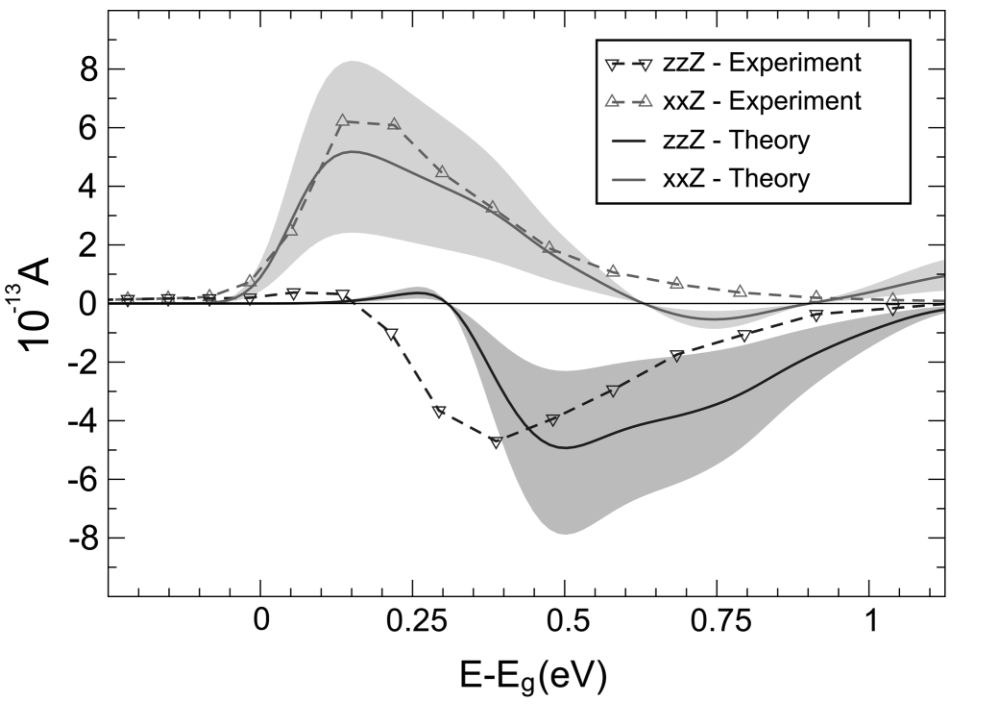
\includegraphics[width=1.0\textwidth]{../figures/young-shift.png}
\caption{BaTiO$_3$的不同方向的位移电流的理论和实验值\cite{koch_anomalous_1976}对比。实线是理论值,虚线是实验值。灰色部分是由于实验样品尺寸的不确定性导致的卢纶值的不确定范围。本图来自文献\onlinecite{young2012}。 注意:该文和本论文采用的符号不一致。本文中的$\sigma^{\alpha\beta\beta}$相当于文献\onlinecite{young2012}中的$\sigma^{\beta\beta\alpha}$(见图例)。\label{young-shift}}
\end{figure}

最早的和实验进行对比的位移电流的计算出现2012年,Steve Young等人\cite{young2012}通过第一型原理方法计算了BaTiO$_3$的位移电流。BaTiO$_3$是典型的铁电材料,具有较大的极化。Steve Young等人和更早期的实验进行了对比,得到了相对比较满意的结果(图\ref{young-shift})。

自此之后,出于实际应用的目的,人们开始探索什么样的材料能够具有较大的位移电流。Cook等人\cite{cook_design_2017}通过建立紧束缚模型并且调节模型参数,推荐了单层$GeS$作为具有较大位移电流的材料。Fregoso等人\cite{fregoso_quantitative_2016}提出,在一定条件下,位移矢量的平均值就是导带和价带的极化差,指出了极化和位移电流存在着非常紧密的关系。但是在实际计算中,人们发现位移电流并不是随着极化的增长单调上升的。后来,Tan等人\cite{tan_upper_2017}提出位移电流存在上限,这个上限正比于紧束缚模型的跃迁参数和带隙的比值的平方。但是这个上限仍然是理想化模型化的,实际材料中的紧束缚模型跃迁参数并不是一个容易确定的数值。Tan等人还尝试对位移电流进行了高通量计算,从中找出了一些位移电流比较大的材料。


\section{布洛赫电子的磁性质}

与电场相比,布洛赫电子的磁性质的研究要困难许多。在一定的规范下,电场可以不破坏晶体的离散平移对称性。但是无论选取什么规范,磁场一定会破坏晶体的离散平移对称性。因此,布洛赫电子在磁场中的运动往往在磁场非常小的情况下进行近似。这个近似在绝大部分实验条件下都是非常合理的。磁场作为小量的理论在这里被称为准经典理论。

人们早已知道,自由电子在磁场中的能级是分立的,这些能级被称为朗道能级。在晶体中,电子的表现是相似的。在费米面没有穿过布里渊区边界的情况下,电子的能级也是分立的,这些能级同样被称为朗道能级。Peierls-Onsager-Lifshitz准经典理论\cite{lifshitz_kosevich,lifshitz_kosevich_jetp}就是一个求解磁场中布洛赫电子的朗道能级和朗道能级波函数的理论,随着磁场变小,Peierls-Onsager-Lifshitz准经典理论越来越精确。Peierls-Onsager-Lifshitz准经典理论的强大之处在于,这个理论仅仅需要知道零场下的电子的能带结构信息,就可以预测出弱磁场下的晶体的各种性质。我们在本文中仅仅讨论等能面闭合的情况,等能面穿过布里渊区的问题留到以后进行研究。由于磁场并不破坏沿着磁场施加方向的离散平移对称性,三维材料在磁场中可以看成二维能带的简单组合。因此在本文中,如果没有特殊说明,我们只讨论二维材料。另外,如果没有特殊说明,我们默认磁场沿着$-z$方向,这样的设定让电子型的载流子会(从$z$方向看过去)逆时针作回旋运动。

在最简单的物理图像下,电子在磁场中会沿着等能面做回旋运动,此时这个电子被称为磁振子。磁振子的运动方程为
\begin{equation}
\hbar\dot{\bk}=-\frac{e}{\hbar}\nabla_{\bk}\epsilon\times\boldsymbol{B}.
\end{equation}
这里$\epsilon$是能带能量。这个回旋运动的周期我们称为磁振子的周期,记为$T_c$.
\begin{equation}
T_c=\frac{1}{\hbar l^2 |dS/dE|}.
\end{equation}
这里,$S$是能量为$E$的等能面的面积。我们同时在这里引入磁长度的概念
\begin{equation}
l=\sqrt{\frac{\hbar}{eB}}.
\end{equation}
磁长度的物理含义是电子在磁场中运动,大概获得$2\pi$的相位所需要运动的长度。在磁场是一个小量的假设下,磁长度$l$是一个大量。磁振子的能量定义为
\begin{equation}
\epsilon_c=\frac{h}{T_c}=\hbar \omega_c.
\end{equation}
磁振子能量刻画了朗道能级的间隔。除此之外,我们还要引入磁振子质量$m_c$
\begin{equation}
\epsilon_c = \hbar^2/m_c l^2.
\end{equation}
对于自由电子,$m_c=m_0$,其中$m_0$就是自由电子的质量。


更加严格的理论则是基于有哈密顿量理论\cite{rotheffham}。这个理论将哈密顿量中的磁场小量展开,在一组合适的基下表示出来。有效哈密顿量理论既可以在实空间表述,也可以在$\bk$空间表述。在零阶近似下,有效哈密顿量在$\bk$空间的表述叫做Peierls替换:将能带能量$\epsilon(\bk)$直接替换为$\epsilon(\bK)$,这里,$\bK=\bk+(e/\hbar)\boldsymbol{A}(i\nabla_{\bk})$。这里的$\epsilon(\bK)$是一个算符,作用在$\bk$空间的波函数上,定态薛定谔方程就变成了
\begin{equation}
\epsilon(\bK)f(\bk)=Ef(\bk).
\end{equation}
这个定态薛定谔方程可以用WKB近似得到近似解。近似解最方便的表达方式是量子化条件,量子化条件是一个关于能量$E$和磁场$B$的方程,这个方程的解就是朗道能级。在零阶近似下,量子化条件是
\begin{equation}
l^2 S=2\pi n+\pi.
\end{equation}
这里的$n$是整数,$\pi$被称为Maslov相位,来自于WKB的量子修正。Maslov相位等于$\pi$仅仅在等能面可以连续变化为圆的时候才成立。这个量子化条件E和B的依赖分别来自于等能面面积$S$和磁长度$l$.

近年来,随着凝聚态中拓扑性质的发现,人们逐渐意识到除了动力学相位之外,几何相位\cite{berry_quantal_1984}同样非常重要。几何相位在量子化条件中贡献的是一阶项。事实上,除了几何相位之外,量子化条件中的一阶项还由轨道磁矩和自旋磁矩贡献。在磁场中,这些磁矩会带来额外的能级移动,从而产生额外的相位。

这些额外的能量在有效哈密顿量里面表现为修正项$\mathfrak{h}_1(\bK)$, 这里。
\begin{equation}
\mathfrak{h}_1(\bk)=B(M^z-g_s\mu_Bs^z/\hbar+e\epsilon^{\alpha\beta}\berry^\beta v^\alpha),
\end{equation}
其中$M^z$是前述的轨道磁矩,$g_s$是自由电子的$g$因子,$\mu_B$是波尔磁子,$s^z$是$z$方向的自旋,$\boldsymbol{v}$是能带速度。

在考虑进这些修正之后,量子化条件改变为
\begin{equation}
l^2 S+\lambda = 2\pi n +\pi\label{single-quan},
\end{equation}
其中
\begin{equation}
\lambda = il^2\oint \frac{\mathfrak{h}_1}{\hbar v^x} dk^y.
\end{equation}
这里积分路径逆时针沿着磁振子轨道。注意$\lambda$和磁场无关,仅仅和能量有关。


以上介绍的是单能带电子的量子化条件。单能带电子指的是在等能面上这个能带处处不简并,并且能隙全部都远大于磁振子能量$\epsilon_c$。如果这个条件不成立,那么量子化条件就需要做出相应的改变。一个典型的情况是能带在布里渊区的一个小区域和其他能带接近简并,这样的情况就会发生磁隧穿现象。如果一个能带处处和其他能带接近简并,那么量子化条件需要做更加复杂的修改,这是本文的研究重点之一。

\subsection{量子振荡}

在磁场中的材料的各种性质会随着磁场的倒数$1/B$周期性振荡,这样的振荡现象被称为量子振荡。最著名的两个量子振荡是de Haas-van Alphen(dHvA)振荡\cite{dHvA}和Shubnikov–de Haas(SdH)振荡\cite{SdH}。dHvA振荡指的是磁矩(或者磁化率)随着磁场的振荡,而SdH振荡指的是电阻随着磁场的振荡。

\begin{figure}
	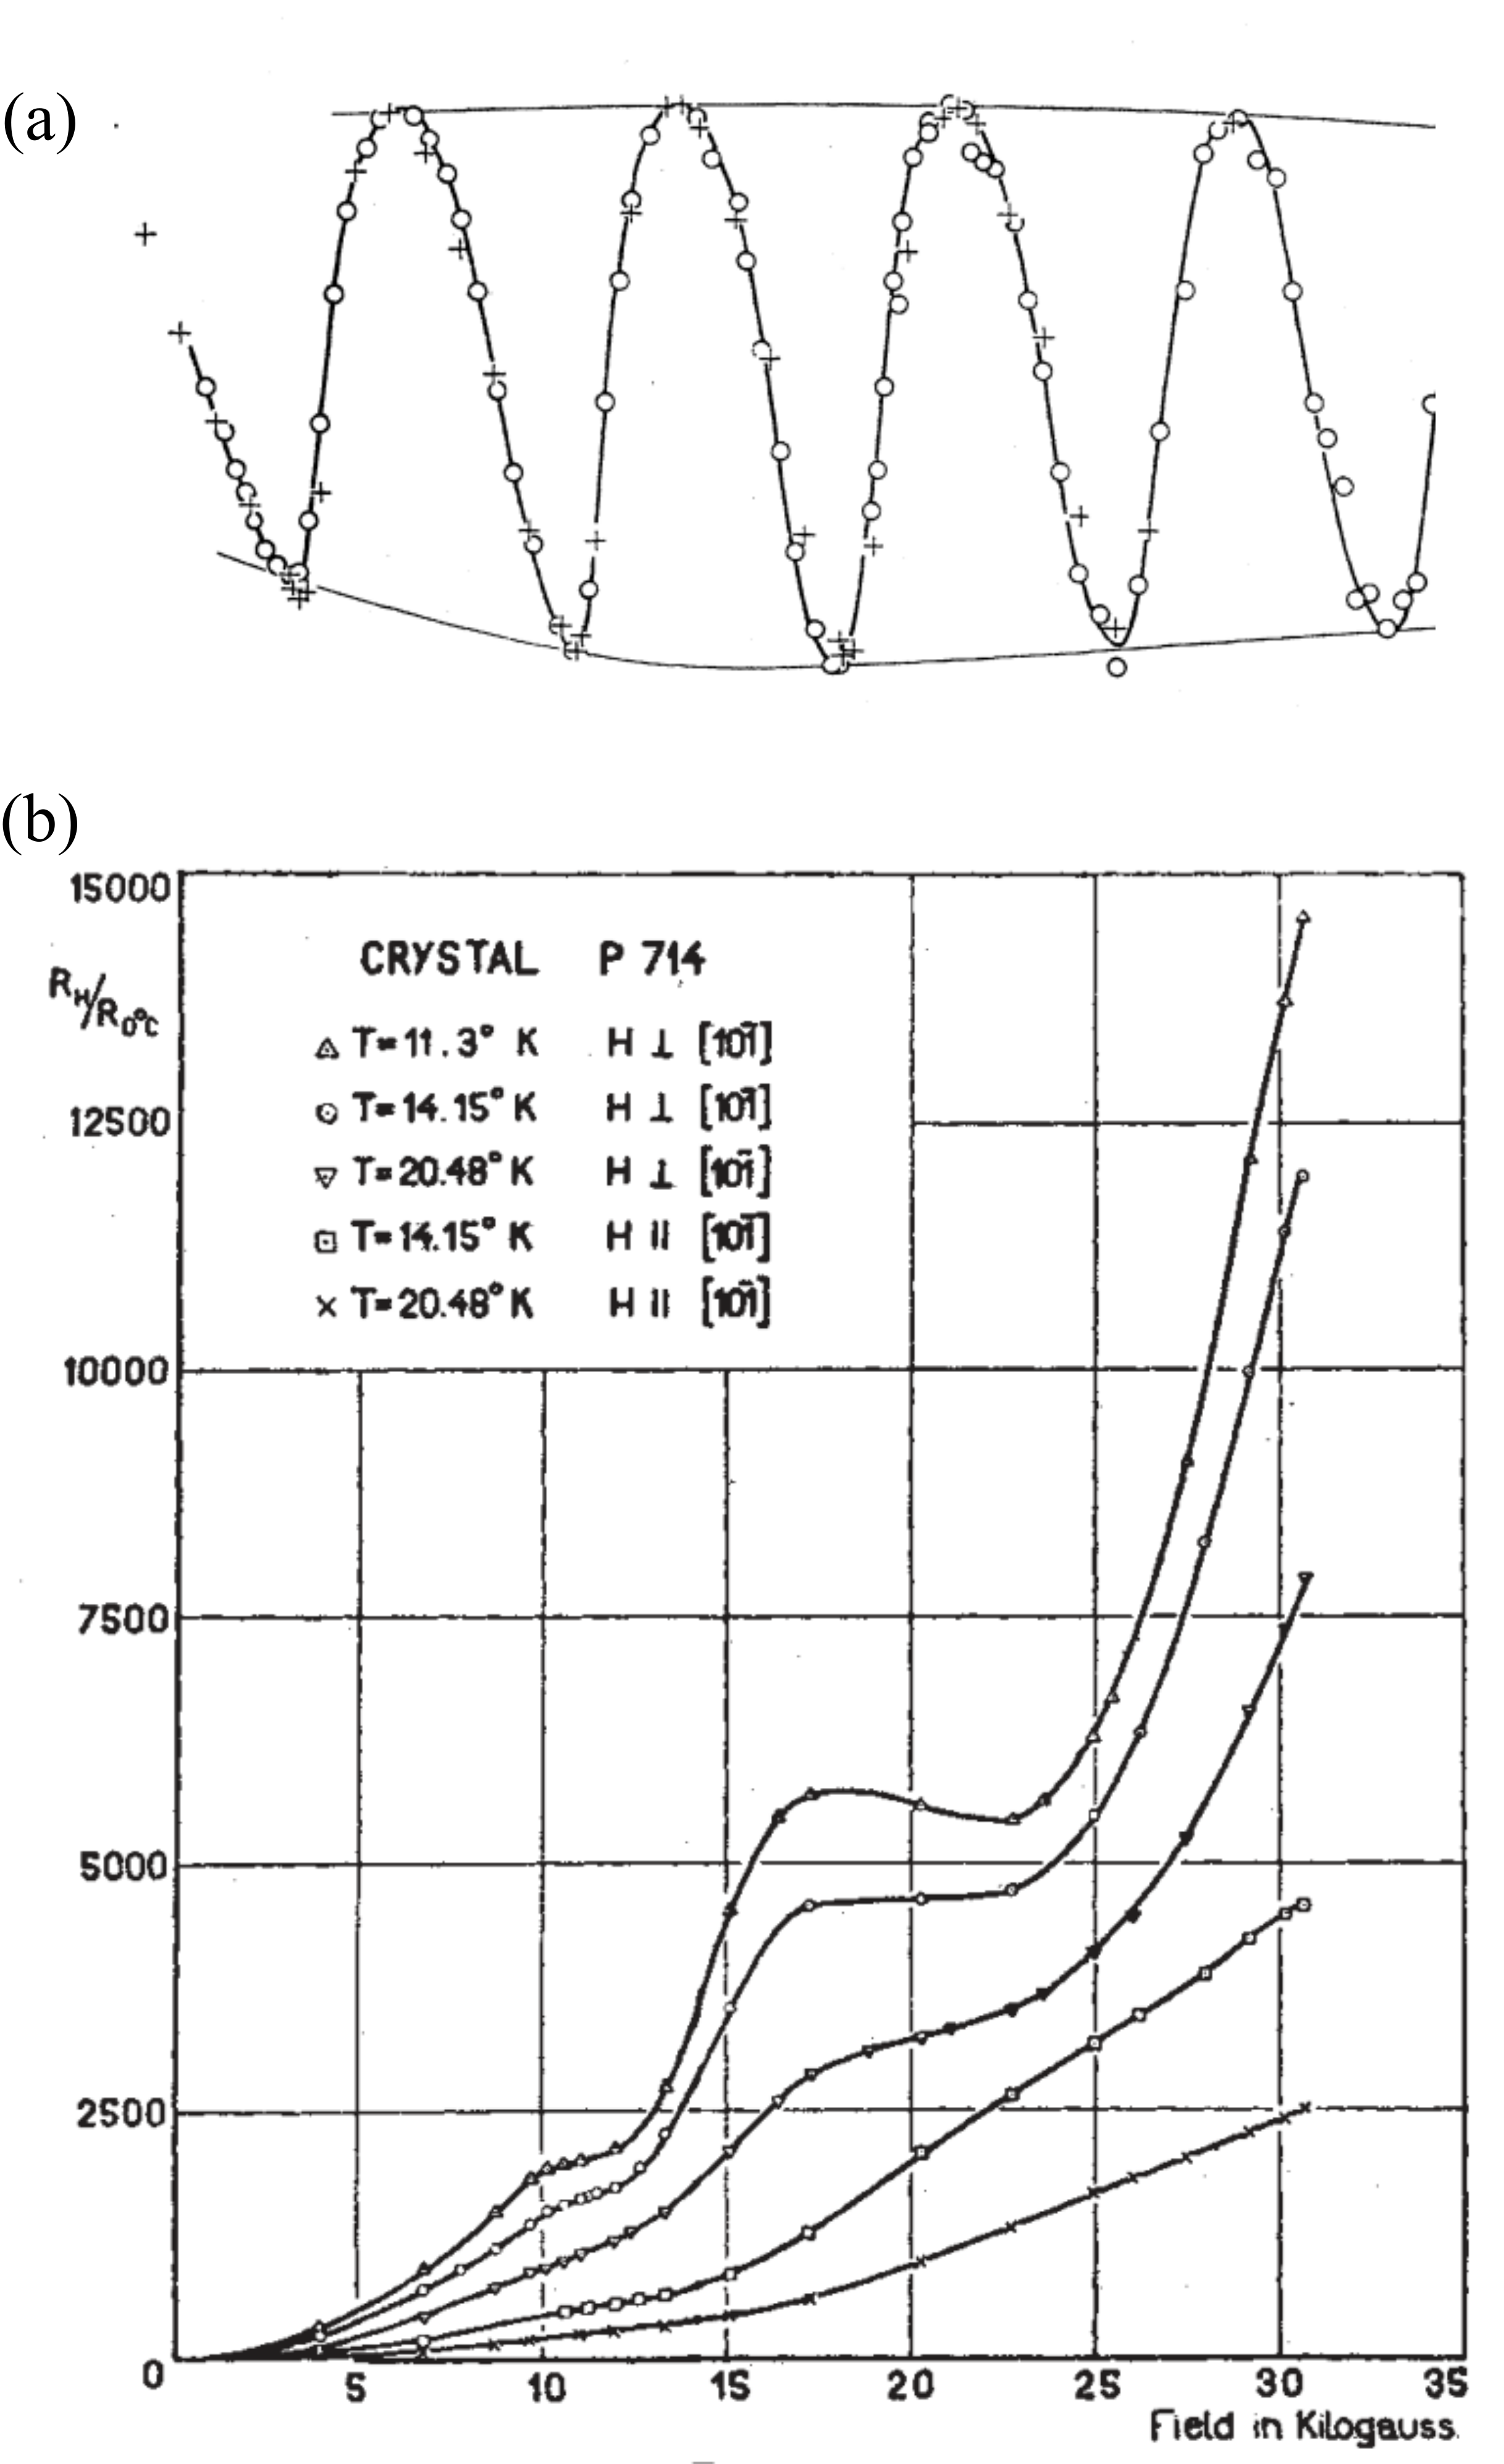
\includegraphics[width=1.0\textwidth]{../figures/quantum-oscillation.png}
	\caption{dHvA振荡(a)和SdH振荡(b). (a)图中横坐标为磁场,纵坐标为$\delta M/B$.\label{quantum-oscillation}}
\end{figure}

量子振荡的基本起源是朗道能级的分立性。随着磁场的变化,朗道能级的能量也会发生变化。当朗道能级穿过费米面的时候,材料的各种性质都会发生比较明显的变化,从而产生振荡效应。将式\ref{single-quan}中的能量取定为费米能,我们可以得到,朗道能级穿过费米面这一事件是随着$l^2$,也就是$1/B$周期发生的,因此量子振荡是随着$1/B$周期性振荡的。

Landau和Lifshitz给出了量子振荡的具体的表达式。一般而言,我们认为电阻正比于费米面处的态密度,所以SdH振荡就正比于态密度振荡。在费米面附近态密度振荡部分的表达式为
\begin{equation}
\delta\nu (E) = \left. \frac{1}{4\pi^3}\frac{\hbar^2}{m_c}\left(\frac{\partial S}{\partial E}\right)^2\sum_{r=1}^{\infty} e^{-r\pi/\omega_c\tau}
\cos [r(l^2 S+\lambda+\pi)] \right|_{E=E_F}.
\end{equation}
这里, $\tau$是Diggle散射时长,代表了杂质的作用。所有的量都是在费米能处计算的。

对于dHvA振荡而言,磁矩的振荡来源于自由能的振荡
\begin{equation}
\delta M = \left. -\frac{1}{2\pi}\frac{k_B T}{B} S\sum_{r=1}^{\infty}e^{-r\pi/\omega_c\tau}\frac{\sin[r(l^2 S+\lambda+\pi)]}{\sinh(2\pi^2 r k_B T/\hbar \omega_c)}\right|_{E=E_F}.
\end{equation}
这里$T$是温度,$k_B$是玻尔兹曼常数。

一般而言,在实验条件下,只有最低阶的振荡($r=1$的振荡)可以被观察到。这种情况下,dHvA振荡和SdH振荡的周期都是反比于费米圆的面积。因此,量子振荡最重要的应用便是测量费米圆的大小。除此之外,我们看到$\lambda$在量子振荡中表现为相位,因此,$\lambda$也是一个可以测量的物理量。$\lambda$体现了费米面处波函数的拓扑性质,近些年来为实验所关注。
\chapter{理论方法}
\label{cha:method}

\section{密度泛函理论}

密度泛函理论是为数不多的能够从量子力学出发,直接预言宏观材料性质的理论之一。密度泛函理论的基础部分在1964被提出\cite{hohenberg_inhomogeneous_1964},指出了多电子相互作用体系可以用其基态的电荷密度唯一确定。1965年,Khon和Sham\cite{kohn_self-consistent_1965}基于密度泛函理论,提出了Khon-Sham方程,使得多电子相互作用的基态的数值计算方法成为可能。如今,密度泛函理论被广泛地运用在凝聚态物理,材料物理,量子化学等领域,大量的基于密度泛函理论的第一性原理软件包也纷纷出现。近些年,人们还采用密度泛函原理对已知的材料进行扫测(也就是高通量计算),为功能材料的工业应用打下了良好的基础。由于密度泛函理论的文献极多,我们仅仅在这里对密度泛函的原理作一个极其简要的介绍。

密度泛函理论的基础包含两个定理,第一个是:对于任何在外场$V_{\text{ext}}(\br)$中的多例子系统,其基态电荷密度能够唯一决定$V_{\text{ext}}(\br)$。

如果基态电荷密度决定了$V_{\text{ext}}(\br)$,那也就决定了整个哈密顿量,也就决定了整个系统的性质,因此基态电荷密度是一个多电子系统决定性的性质。

第二个定理是,定义泛函
\begin{equation}
    E[n] = \text{min}_{\Psi\to n} \{\langle\Psi|\hat{H}_0|\Psi\rangle\}+\int V_\text{ext}(\br) n(\br) d\br
\end{equation}
则在固定$V_\text{ext}$的情况下,$E[n]$的最小值就是对应的基态电荷密度。这里$\hat{H}_0$是不含外场的哈密顿量。$\Psi\to n$指的是在满足电荷密度为$n(\br)$的波函数$\Psi$中进行最小化。

在这种情况下,如果我们得知了$E[n]$,或者$E[n]$的近似形式,就可以通过最优化得到基态电荷密度。

优化上述的泛函的方法由Khon和Sham给出。Khon和Sham假设,这个相互作用的多电子体系的基态电荷密度可以用一个无相互作用系统的基态电荷密度给出,从这个假设可以推导出Khon-Sham方程。Khon-Sham方程是一个自洽方程,其独立粒子势能需要用态密度得到,这样就构成了势能到波函数到态密度再到势能的闭合循环。这个自洽迭代就可以解出最后的基态能量。不过Khon和Sham的上述假设并没有得到严格证明。

下面我们来介绍一下与本文更加相关的最大局域化方法Wannier函数方法。

\section{最大局域化Wannier方法}
\subsection{引言}
凝聚态物理学中,常用的近似是近独立粒子近似。在这个近似下,可以用一系列单粒子波函数的集合以及其占据数来描述固体系统的基态,
在周期势场下,单粒子波函数通常取作布洛赫波函数$\psi_{n\bm{k}}$,其中n是能带的带序,$\bm{k}$是布里渊区的晶格准动量。虽然,布洛赫波表象是电子结构计算中最常用,但是由于布洛赫波函数具有延展性会带来计算的难度,另外一种表象—瓦尼尔表象通常被采用。瓦尼尔(Wanier)表象中的瓦尼尔函数$w_{n\bm{R}}$可以通过一个幺正变换和布洛赫波函数联系,是由瓦尼尔最早提出的。瓦尼尔函数由晶格矢量$\bm{R}$和能带带序的n来标记。

虽然瓦尼尔函数一直被提到,但是真正植入用于第一性原理计算却经历了很大的困难。一个主要的原因是由于洛赫波函数$\psi_{n\bm{k}}$在每个$\bm{k}$点的相位随机性带来的瓦尼尔函数不唯一,或者说是由于对各个$\bm{k}$点的布洛赫波函数作幺正变换的时候规范不确定性带来的瓦尼尔函数的不唯一。这种规范不确定性的困难尤其在碰到简并能带的时候尤为棘手,因为当把简并的能带划分成分开的能带变换到瓦尼尔函数时,是很有问题的。一个非常重要的发展是Marzari和Vanderbilt\cite{marzari_maximally_2012}在1997年提出在给定一个绝缘体后用“最大局域化”的标准来唯一决定一组瓦尼尔函数。紧接着,Souza, Marzari和Vanderbilt\cite{souza_maximally-localized_2001}又提出一种办法来解决构造一组可以张成一个子空间的瓦尼尔函数的问题,这个方法可以处理具有部分占据能带的金属。

在这个重大的发展后,一大批从事电子结构计算的研究者把最大局域化瓦尼尔函数方法用于计算各种各样的性质,并且他们为此发展了一系列后处理程序。更有趣的是,瓦尼尔函数的中心电荷和布洛赫波函数的贝里曲率紧紧联系在一起,这个联系在现代极化理论中被提出,使得人们更好地理解了材料的介电性质和极化\cite{king-smith_theory_1993}。凝聚态物理中更常用的是用瓦尼尔函数来构造关联电子系统和磁性系统的模型哈密顿量。其他的应用还包括在弹道输运理论中用瓦尼尔基组来构造格林函数以及其自能,或者用瓦尼尔基组在化学精度上来精确构造第一性紧束缚计算哈密顿量。最后,值得一提的是,瓦尼尔函数还被用于声子,声子晶体,冷原子晶格以及绝缘体的局域介电响应的理论分析。

\subsection{基础理论}
在对周期性体系进行电子结构的计算的时候,单电子有效哈密顿量$H$和晶格矢量平移算符$T_{R}$对易,因此布洛赫波函数可以被表示为一个周期性函数$u_{n\bm{k}}$加上一个相位调制:
\begin{equation}
[H,T_{R}]=0\Rightarrow \psi_{n\bm{k}}=u_{n\bm{k}}e^{i \bm{k} \cdot \bm{r}}
\end{equation}
我们用$\bm{R}n$来标记局域在晶胞$\bm{R}$的第n调带的瓦尼尔函数$w_{n\bm{R}}$,采用狄拉克符号标记,瓦尼尔函数可以用以下方式来构造
\begin{equation}
|\bm{R}n \rangle= \frac{V}{(2\pi)^3}\int_{BZ}d\bm{k}e^{-i\bm{k}\cdot\bm{R}}|\psi_{n\bm{k}}\rangle
\end{equation}
显而易见,所有的$|\bm{R}n \rangle$构成了一个正交集。等式(3)是一个傅里叶变换,它的逆傅里叶变换是:
\begin{equation}
|\psi_{n\bm{k}}\rangle= \sum_{\bm{R}}e^{i\bm{k}\cdot\bm{R}}|\bm{R}n \rangle
\end{equation}
瓦尼尔函数和布洛赫函数通过等式(2)和(3)相互联系,因此在某一个能带子空间内这两种描述方法是等价的,这种等价性也体现在投影算符上:
\begin{equation}
P= \frac{V}{(2\pi)^3} \int_{BZ}d\bm{k}  |\psi_{n\bm{k}}\rangle \langle\psi_{n\bm{k}} |=\sum_{\bm{R}}|\bm{R}n \rangle \langle \bm {R}n |
\end{equation}
\subsubsection{规范问题}
我们可以改写布洛赫波函数
\begin{equation}
|\widetilde \psi_{n\bm{k}}\rangle= e^{i \varphi_{n}(\bm{k})} |\psi_{n\bm{k}}\rangle
\end{equation}
或者等效得,
\begin{equation}
|\widetilde u_{n\bm{k}}\rangle= e^{i \varphi_{n}(\bm{k})} |u_{n\bm{k}}\rangle
\end{equation}
但是不会对系统的课观测量有任何的转变,这在前文已经提到,即布洛赫函数具有随机性,即给布洛赫函数加一个相位并不改变物理观察量。结合等式(6)和(7)就可以发现,这样的规范不确定性使得得到的瓦尼尔函数不唯一,不同的规范会得到不同的瓦尼尔函数。值得一提的是,对于从薛定谔方程解得的布洛赫函数来说,其并没有一个所谓的最佳规范,因此相位的选择是随机的,这就不可避免地造成了瓦尼尔函数的不唯一性。
\subsubsection{多带问题}
在讨论如何解决瓦尼尔函数的不确定性之前,我们先讨论多带的情况,比如由J条能带组成的一个流形,流形内的能带和流形外的能带是分开的。不失一般性的,流形内的能带可以存在简并或者交叉。在这个有J条带构成的流形内,我们依然可以通过规范变换来改写波函数:
\begin{equation}
|\widetilde \psi_{n\bm{k}}\rangle= \sum_{m=1}^{J}U^{(\bm{k})}_{mn} |\psi_{n\bm{k}}\rangle
\end{equation}
其中,$U^{(\bm{k})}_{mn}$ 是一个J维的在$\bm{k}$空间具有周期性的幺正矩阵。$\bm{k}$的投影算符在这个能带流型下是规范不变的:
\begin{equation}
P_{\bm{k}}= \sum_{n=1}^{J}|\psi_{n\bm{k}}\rangle \langle\psi_{n\bm{k}} |= \sum_{n=1}^{J}|\widetilde\psi_{n\bm{k}}\rangle \langle\widetilde \psi_{n\bm{k}} |
\end{equation}
我们要再次强调在多带情况下,规范不确定性更加加剧了瓦尼尔函数的不唯一性。更严重的问题是,当简并能带存在时,布洛赫波函数在简并点附近是不解析的,这种情况下继续利用等式(2)作傅里叶变换会得到局域性很差的瓦尼尔函数。
总的来说,得到瓦尼尔函数有这么几个步骤:首先得到本身不平滑的哈密顿量的本征态$|\psi_{n\bm{k}}\rangle$,然后通过规范变换$U^{(\bm{k})}_{mn}$得到$|\widetilde\psi_{n\bm{k}}\rangle$来消除不连续性以保持其平滑性。然后把$|\widetilde\psi_{n\bm{k}}\rangle$代入到等式(2)来得到瓦尼尔函数。更具体地说,这样得到的瓦尼尔函数具有如下形式:
\begin{equation}
|\bm{R}n \rangle=\frac{V}{(2\pi)^3} \int_{BZ}d\bm{k} e^{-i\bm{k}\cdot\bm{R}} \sum_{m=1}^{J}U^{(\bm{k})}_{mn}|\psi_{m\bm{k}}\rangle
\end{equation}
剩下的问题就是如何选择$U^{(\bm{k})}_{mn}$来完成这个任务。

\subsection{投影瓦尼尔函数}
一个简单的常见消除不连续性得到平滑规范的方法是通过投影得到的瓦尼尔函数。Marzari 和Vanderbitz提出,可以在初始的时候猜一些轨道$g_{n}(\bm{r})$。在每个$\bm{k}$点,这些 初始轨道$g_{n}(\bm{r})$可以被投影到一个布洛赫流形:
\begin{equation}
|\phi_{n\bm{k}}\rangle=\sum_{m=1}^{J}|\phi_{m\bm{k}}\rangle \langle \phi_{m\bm{k}}|g_{n}\rangle
\end{equation}
这样得到的波函数$|\phi_n\bm{k}\rangle$虽然不正交,但是在$\bm{k}$空间是平滑的。我们通常定义内积$(A_{\bm{k}})_{mn}=\langle \phi_{m\bm{k}}|g_{n}\rangle$,然后代入等式(10)。利用交叠矩阵$(S_{\bm{k}})_{mn}=\langle \phi_{m\bm{k}}| \phi_{m\bm{k}}\rangle_V=(A^\dagger_{\bm{k}}A_{\bm{k}})_{mn}$(其中V代表对一个原胞进行积分),我们得到
\begin{equation}
|\widetilde\psi_{n\bm{k}}\rangle=\sum_{m=1}^{J}|\phi_{m\bm{k}}\rangle (S^{-1/2}_{\bm{k}})_{mn}
\end{equation}
这些和$|\widetilde\psi_{n\bm{k}}\rangle$同过幺正变换相联系的波函数$|\widetilde\psi_{n\bm{k}}\rangle$在$\bm{k}$空间是平滑的。这样我们就消除了规范不确定性问题。

需要强调的是,一开始猜测的波函数不需要很接近目标瓦尼尔函数,一开始选择一些简单的轨道就已经足够了,只要他们大致局域在原子位置上。只要我们得到的内积矩阵$(A_{\bm{k}})_{mn}$在任何$\bm{k}$点没有奇点,这个方法就是成功的。关于$(A_{\bm{k}})_{mn}$有没有奇点,我们可以通过$(S_{\bm{k}})_{mn}$最大值和最小值得比例是否过大来检查。

\subsection{最大局域化瓦尼尔函数}
上一节提到的投影瓦尼尔函数有着广泛地应用,但是最受欢迎的一种用法是所谓的最大局域化瓦尼尔波函数。最大局域化瓦尼尔波函数通过设定一个有良好定义的局域化判据来构造瓦尼尔波函数的时候,具体体现在重新定义$U^{(\bm{k})}_{mn}$来满足这个判据。

首先,我们定义一个局域化函数来衡量J个瓦尼尔函数的速度的平方和:
\begin{equation}
\Omega=\sum_n [\langle\bm{0} n | r^2 | \bm{0}n \rangle -\langle \bm{0}n|\bm{r}|\bm{0}n\rangle^2]=\sum_n[\langle r^2\rangle_n-\bm{\overline r}^2_n]
\end{equation}
下一步是用布洛赫波函数来表达$\Omega$.

一旦$\bm{k}$空间的$\Omega$的表达式得到后,就可以选择$U^{(\bm{k})}_{mn}$来最小化$\bm{k}$空间的$\Omega$以得到最大局域化的瓦尼尔波函数。这一步是在通常的电子结构的自洽计算已经完成的基础上后处理得到。


\subsubsection{实空间表示}
我们把等式(12)的$\Omega$分为规范不变的部分和规范依赖的部分:
\begin{equation}
\Omega=\Omega_I+\widetilde\Omega
\end{equation}
其中
\begin{equation}
\Omega_I=\sum_n [\langle\bm{0} n | r^2 | \bm{0}n \rangle -\sum_{\bm{R}m}|\langle \bm{R}m|\bm{r}|\bm{0}n\rangle|^2] 
\end{equation}

\begin{equation}
\widetilde \Omega=\sum_n \sum_{\bm{R}m\neq \bm{0}m}|\langle \bm{R}m|\bm{r}|\bm{0}n\rangle|^2
\end{equation}
可以看到,$\Omega_I$和$ \widetilde \Omega$都是正定的,其中$\Omega_I$是规范不变的,即无论等式(7)取什么样的规范,它都是不变了。通过在等式(8)定义的投影算符$P$重写等式(13)是十分直接的,我们定义$Q=1-P$,然后我们又有:
\begin{equation}
\Omega_I=\sum_{n\alpha} \langle\bm{0} n | r_\alpha Q  r_\alpha  | \bm{0}n \rangle=\sum_\alpha Tr_c[P r_\alpha Q r_\alpha]
\end{equation}
其中下指标“c” 表示对每一个单位原胞求迹。很显然的,$\Omega_I$是规范不变的,因为它可以通过投影算符表达出来,而投影算符是不依赖于规范的选取的。既然$\Omega_I$是规范不变的,那么所谓的最小化进程就是通过规范选取来最小化规范依赖的$ \widetilde \Omega$部分。

\subsubsection{倒空间表示}
位置算符在瓦尼尔表象下的形式:
\begin{equation}
\langle \bm{R}n |\bm{r}|\bm{0}m\rangle=i \frac{V}{(2\pi)^3}\int d\bm{k} e^{i \bm{k} \cdot \bm{R}} \langle u_{n \bm{k}}| \nabla_{\bm{k}}| u_{m \bm{k}}\rangle
\end{equation}
位置算符的平方在瓦尼尔表象下的表现形式:
\begin{equation}
\langle \bm{R}n |\bm{r^2}|\bm{0}m\rangle=- \frac{V}{(2\pi)^3}\int d\bm{k} e^{i \bm{k} \cdot \bm{R}} \langle u_{n \bm{k}}| \nabla^2_{\bm{k}}| u_{m \bm{k}}\rangle
\end{equation}
由于这两个关系式把局域化函数的矩阵元用$\nabla_{\bm{k}}$和$ \nabla^2_{\bm{k}}$表达,所以它们是联系瓦尼尔表象和布洛赫表象的重要的桥梁。另外,它们还使得计算$|u_{n\bm{k}}\rangle$在任意幺正变换下的局域性效应不需要进行任何昂贵的标量积计算。我们可以在一个规则的网格上撒$\bm{k}$点,计算每个$\bm{k}$点上的布洛赫轨道$|u_{m\bm{k}}\rangle$以及通过差分的办法来得到上式中的微分项。

对于在$\bm{k}$空间上平滑的任何函数$f(\bm{k})$,它的梯度可以用有限差分的方法表现为:

\begin{equation}
\nabla f(\bm{k})=\sum_{\bm{b}}\omega_b\bm{b}[f(\bm{k}+\bm{b})-f(\bm{k})]+\mathcal{O}(b^2)
\end{equation}
这里$\bm{b}$是连接$\bm{k}$和其邻近点的矢量,$\omega_b$是一个几何因子。类似的:
\begin{equation}
|\nabla f(\bm{k})|^2=\sum_{\bm{b}}\omega_b[f(\bm{k}+\bm{b})-f(\bm{k})]^2+\mathcal{O}(b^3)
\end{equation}
有了等式(19)和等式(20)以后,计算等式(17)和(18)就变得十分直接。所有需要的关于倒格矢空间的微分项的信息都包含在一个描述相邻$\bm{k}$点布洛赫波的交叠矩阵里面:
\begin{equation}
M^{(\bm{k},\bm{b})}_{mn}=\langle u_{m \bm{k}}|u_{n,\bm{k}+\bm{b}} \rangle
\end{equation}
这个交叠矩阵在瓦尼尔方法中是十分重要的,因为所有的对局域化函数的贡献都可以用这个交叠矩阵来表达。因此,一旦得到这个交叠矩阵$(M^{\bm{k},\bm{b}}_{mn})$被得到以后,额外的用电子结构计算软件计算基态波函数的步骤都是不必要的,这就使得瓦尼尔化进程是一个不依赖于特定程序或者代码的后处理的进程。
用局交叠矩阵表达局域化函数的方式并不唯一,因为我们有很多种可以选择的方法来写下$\bm{\overline r_n}$和$\langle r^2\rangle_n$的有限差分的表达式。这里我们给出Marzari 和Vandervilt在1997年提出的满足在移动$|\bm{0}n \rangle$一个波矢的规范变换下的有正确变换的表达式:
\begin{equation}
\overline r_{n}=-\frac{1}{N}\sum_{\bm{k},b}\omega_b\bm{b}\ln M^{(\bm{k},b)}_{nn}
\end{equation}
以及
\begin{equation}
\langle r^2\rangle_{n}=\frac{1}{N}\sum_{\bm{k},b}\omega_b{[1-|M^{(\bm{k},b)}_{nn}|^2]+[Im \ln M^{(\bm{k},b)}_{nn} ]^2}
\end{equation}
相应的规范不变的和规范依赖的伸展函数的表达式为:
\begin{equation}
\omega_I=\frac{1}{N}\sum_{\bm{k},\bm{b}}\omega_b(J-\sum_{mn}|M^{(\bm{k},b)}_{nn}|^2)
\end{equation}
和
\begin{equation}
\widetilde \omega=\frac{1}{N}\sum_{\bm{k},\bm{b}}\omega_b\sum_{m \neq n}|M^{(\bm{k},b)}_{nn}|^2+\frac{1}{N}\sum_{\bm{k},\bm{b}}\omega_b\sum_{n}(-Im \ln M^{(\bm{k},b)}_{nn}-\bm{b} \cdot \bm{\overline r_n})
\end{equation}

\subsection{局域化进程}
为了最小化局域化函数,我们考虑做一个来自于无穷小的规范变换对伸展函数$\Omega$的一阶效应的改变,这个无穷小的规范变换为$U^(\bm{k})_{mn}=\delta_{mn}+dW_{mn}^{\bm{k}}$。其中$dW_{mn}^{\bm{k}}$是一个无穷小的反厄米的矩阵,即$dW^\dagger=-dW$,所以有$|u_{n\bm{k}}\rangle\rightarrow |u_{n\bm{k}}\rangle+\sum_mdW_{mn}^{\bm{k}}|u_{m\bm{k}}\rangle$。这里我们约定:
\begin{equation}
(\frac{d\Omega}{dW})_{nm}=\frac{\Omega}{dW_{mn}}
\end{equation}
注意等式两边的m和n的指标互换了。我们引入$\mathcal{A}$和$\mathcal{S}$和相应的超算符 $\mathcal{A}[B]=(B-B^\dagger)/2$以及$\mathcal{S}[B]=(B+B^\dagger)/2i$。我们定义:
\begin{equation}
q^(\bm{k},\bm{b})_n=Im \ln M^(\bm{k},\bm{b})_{nn}+\bm{b} \cdot \overline r_n
\end{equation}

\begin{equation}
q^(\bm{k},\bm{b})_n=Im \ln M^(\bm{k},\bm{b})_{nn}+\bm{b} \cdot \overline r_n
\end{equation}

\begin{equation}
R^{(\bm{k},\bm{b})}_{mn}= M^{(\bm{k},\bm{b})}_{mn}M^{(\bm{k},\bm{b})\ast}_{nn}
\end{equation}
\begin{equation}
T^{(\bm{k},\bm{b})}_{mn}= \frac{M^{(\bm{k},\bm{b})}_{mn}}{M^{(\bm{k},\bm{b})}_{nn}}q^{(\bm{k},\bm{n})}_n
\end{equation}
参考Marzari和Vanderbilt在1997年写的文章,我们可以得到伸展函数$\Omega$的梯度$G^{(\bm{k})}=d\Omega /dW^{(\bm{k})}$的具体表达式:
\begin{equation}
G^{(\bm{k})}=4\sum_{\bm{b}}\omega_b(\mathcal{A}[R^{(\bm{k},\bm{b})}]-\mathcal{S}[T^{(\bm{k},\bm{b})}])
\end{equation}
这个梯度在选取合适的$U_{mn}^{k}$得到$\Omega$的最小值的过程中有重要作用,一个简单的最速下降法是通过朝着梯度$G$的反方向进行有限的步骤直到达到$\Omega$的最小值。

在这里,我们指出,所有的算符都可以用在小矩阵上做不昂贵的矩阵代数运算得到,最消耗计算资源部分的程序是最开始的典型的自洽计算得到布洛赫波函数$|u^{(0)}_{n\bm{k}}$部分,以及之后对一系列交叠矩阵的计算:
\begin{equation}
M_{mn}^{(0)(\bm{k},\bm{b})}=\langle u_{m\bm{k}}^{(0)}|u^{(0)}_{n,\bm{k+b}}\rangle
\end{equation}
这个交叠矩阵只要在布洛赫波函数$|u^{(0)}_{n\bm{k}}$得到后立刻计算出来。之后每进行一次幺正矩阵$U^{(k)}$的选择,这个交叠矩阵只要做相应的不太消耗计算资源的矩阵代数来更新即可:
\begin{equation}
M^{(\bm{k},\bm{b})}=U^{(k)\dagger}M_{mn}^{(0)(\bm{k},\bm{b})}U^{\bm{(k+b)}}
\end{equation}
而不需要任何的布洛赫波函数的计算过程。这种做法不仅使得这个算法在计算上更快更有效,也使得其并不依赖于布洛赫表象中基矢的选取。换句话说,任何电子结构计算的软件包都可以提供一系列的交叠矩阵$M^{(\bm{k},\bm{b})}$和常用的瓦尼尔最大局域化代码很容易得对接。
\subsection{纠缠能带}
前面章节提到的方法都是处理一组隔离的能带,它们和其它能带通过贯穿整个布里渊区的能隙来分离开。但是,很多情况下,我们感兴趣的能带不是分离的,它们和其它能带纠缠在一起。比如说,研究电子输运的时候,起主导作用的是费米面附近部分占据的能带,或者在处理形如四面体结构半导体的四条低能级的反键带的空带(通常是在较高的导带)的时候。另外一个感兴趣的情况是部分占据的能带在瓦尼尔函数表象下实现降维以构造模型哈密顿量。在这些例子里面,虽然感兴趣的能带在一个有限的能量窗口里面但是和窗口外的能带交叠杂化在一起,我们称之为纠缠能带。

处理纠缠能带最大的困难在于我们不知道选取多大的J是合适的,特别是某些$\bm{k}$点我们想要的能带和我们不想要的能带纠缠很严重的时候。在瓦尼尔局域化进程开始之前,在更大的流形中通过态的线性组合来构造每个$\bm{k}$点的J个态的方法是需要的。只要每个$\bm{k}$点的合适的J维的布洛赫流形被得到以后,我们就可以依然用和前面处理隔离能带一样的程序来得到广义的张成所想要流形的局域瓦尼尔函数。

从纠缠态出发得到良好定义的瓦尼尔函数的困难在于两点:子空间的选取和规范的选取。我们可以用同样的指导原则来做两步,那就是实现在$\bm{k}$空间的平滑性。在选取子空间一步,在$\bm{k}$空间平滑的J维的布洛赫流形被构造出来。在规范选取步,采用在子空间选取一步中本身在$\bm{k}$空间平滑的J 个布洛赫波函数构成的子空间,因此,相应的瓦尼尔函数是良好定义的。

\subsubsection{通过投影选取子空间}
我们从J个局域的平凡的轨道$g_n(\bm{r})$构成的集合出发,在给定$\bm{k}$点把它们投影到改$\bm{k}$点张成的空间上:
\begin{equation}
|\phi_{n\bm{k}} \rangle=\sum_{m=1}^{\mathcal{J}_{\bm{k}}}|\psi_{m\bm{k}} \rangle \langle\psi_{m\bm{k}}|g_n \rangle
\end{equation}
这种情况下,交叠矩阵$(A_k)_{mn}=\psi_{m\bm{k}}|g_n \rangle$ 变成了$\mathcal{J}_{\bm{k}} \times J $维的长方形矩阵。然后我们构造
\begin{equation}
|\widetilde\psi_{n\bm{k}}\rangle=\sum_{m=1}^{\mathcal{J}}|\phi_{m\bm{k}} \rangle(S^{-1/2}_{\bm{k}})_{mn}
\end{equation}
以上过程自动实现了子空间的选取和规范选取两步,虽然这样做并不是最理想化的。在规范选取一步还可以进一步选择规范来实现投影子空间的$\widetilde \Omega$的最小化。

\subsubsection{通过最理想平滑选取子空间}
为了优化子空间选择的进程,一个有用的做法是引入具体衡量在$\bm{k}$空间的布洛赫流形的平滑性的标准吗,寻找一个最理想的平滑的子空间可以定义成一个最小化的问题,这和寻找最优化的平滑规范势类似的。

事实上,布洛赫态空间在$\bm{k}$空间的平滑性可以用之前介绍的$\Omega_I$来衡量。前文提到的$\Omega$由规范不变的$\Omega_I$和规范变化的$\widetilde \Omega$组成,给定一个布洛赫空间,我们发现最理想的平滑规范可以通过最小化$\widetilde \Omega$来得到。
我们先得到离散$\bm{k}$空间的$\Omega_I$的表达式
\begin{equation}
\Omega_I=\frac{1}{N}\sum_{\bm{k},\bm{b}}w_bT_{\bm{k},\bm{b}}
\end{equation}
其中
\begin{equation}
T_{\bm{k},\bm{b}}=Tr[P_{\bm{k}}Q_{\bm{k+b}}]
\end{equation}
$P_{\bm{k}}=\sum_{n=1}^{J}|\widetilde u_{n \bm{k}}\rangle \langle\widetilde u_{n \bm{k}}|$是投影到布洛赫子空间的规范不变的算子,$Q_{\bm{k}}=1-P){\bm{k}}$,“Tr”表示在全希尔伯特空间求迹。$T_{\bm{k},\bm{b}}$描述了在$\bm{k}$和$\bm{k+b}$的相邻布洛赫子空间的不匹配性,如果它们一样,那么$T_{\bm{k},\bm{b}}$这一项就会消失。

主要的理想化的子空间选择过程如下:在一定能带范围内确定大于等于$J$的$\mathcal{J}_{\bm{k}}$个布洛赫态的集合。我们把这个能量范围叫做“非纠缠窗口”。然后通过一个自洽的叠代程序来得到最小值$\Omega_I$。在叠代的最小化过程中,最后得到的布洛赫波子空间就是理想化平滑的。通常来说,这个最小化过程从一个初始猜测开始。

\subsection{总结}
本章中我们主要介绍了最大局域化的瓦尼尔方法。最大瓦尼尔方法先通过投影算符的办法得到在$\bm{k}$空间上平滑的布洛赫波函数,再通过最小局域化函数来得到最局域的瓦尼尔函数。如果要处理纠缠带的问题,这可以通过投影或者理想平滑化的方法选择子空间和规范。最大局域化瓦尼尔函数在凝聚态的各个领域都有着重要的应用。
\chapter{非线性光学性质的Wannier插值计算方法}

非线性光学效应在现代光学和现代凝聚态物理中起着非常重要的作用\cite{boyd-nlo}。非线性光学材料在很多领域都有非常重要的实际应用,尤其是激光科学技术领域\cite{nurmikko-compact,kanai_generation_2004,boyd-nlo}。非线性光学材料可以通过频率转换,将现有的激光转换到远红外或者远紫外频率\cite{nurmikko-compact,kanai_generation_2004}。尽管非线性光学研究已经有了半个世纪以上的历史,但是对新奇的非线性光学效应的探索仍然没有停止\cite{young2012,young2012_2,tan2016,morimoto2016,morimoto2016prb,rangel_giant_2016,cook_design_2017,wu_giant_2017}。近几年来,人们逐渐开始研究贝里相位和拓扑效应在非线性光学中的效应\cite{xiao2010,hasan2010,qi2011}。重要的是,最近的理论工作揭示了包括位移电流,倍频效应,光伏霍尔效应等等效应都和拓扑相关的物理量如贝里相位和贝里曲率有关系\cite{morimoto2016,morimoto2016prb}。除此之外,实验和理论都证实了在拓扑材料中的非线性光学效应非常显著\cite{tan2016,wu_giant_2017}。在这样的背景下,研究非线性光学现象中的拓扑效应就成为了非常重要的课题。

在材料科学领域,第一性原理方法非常有效,不可替代。第一性原理方法能够在不引入任何经验参数的情况下计算材料的各种性质。现如今,人们多次使用第一性原理方法计算非线性光学效应\cite{sipe_second-order_2000,young2012,rangel_giant_2016,cook_design_2017}。但是,这些方法计算量都非常地大,布里渊区的积分需要极密的$k$点。另外一方面,第一性原理生成的波函数的相位不确定性,如果没有得到很好的处理,将无法计算贝里相位和贝里相位的导数。这个问题被称为相位问题。要解决这些问题,人们需要新的计算非线性光学效应的方法。最近,基于Mazari等人提出的最大局域化Wannier函数方法\cite{marzari_maximally_1997,marzari2012},Wannier插值方法被用来计算各种各样的物理量,包括反常霍尔电导,轨道磁矩等等\cite{wang_textitab_2006,yates_spectral_2007,lopez_wannier-based_2012}。这些计算采用一阶微扰来解决相位问题。Wannier插值方法计算量很小,并且可以和绝大部分第一性原理计算方法接口,包括密度泛函理论,杂化泛函和$GW$方法。但是,据我们所知,并没有人尝试用Wannier插值方法计算非线性光学效应。


我们在这里将Wannier插值方法推广,用以计算非线性光学效应。这个方法通过二阶微扰构建了一个平滑的相位规范,可以准确计算任何$k$点的波函数的导数和二阶导数。作为示例,我们计算了单层GeS和WS$_2$的位移电流,以及GaAs的倍频效应,得到了和前人一致的结果\cite{rangel_giant_2016,nastos_scissors_2005}。我们同时证明了基于微扰的Wannier插值方法优于传统基于波函数的计算方法。传统方法利用了一些近似的求和规则\cite{sipe_second-order_2000,cook_design_2017},需要对所有能带进行求和,其收敛相对较慢。最后我们提出Wannier插值可以很容易地被用来构建紧束缚模型,方便理论地研究。这些优点让Wannier插值成为一个在非线性光学领域很有前景的计算方法。


\section{计算方法}
\subsection{相位问题}

由于布洛赫波函数存在着相位不确定性,在计算布洛赫波函数的导数的过程中,我们需要非常的小心。在第一性原理中,布洛赫波的相位一般而言是随机的,由于有限差分方法仅适用于连续可导的函数,贝里联络不能够采用有限差分的方法进行计算。这个问题被称为相位规范问题。在计算非线性光学的过程中,相位问题必须小心处理。据我们所知,目前有两种方案来处理相位问题,其中一种是构造规范不变的离散表达式,另外一种是采用动量矩阵和求和规则。下面我们对这两种方式进行简单的介绍。


\subsection{构造规范不变的表达式}

任何物理量归根结底不应该依赖于规范的选区,这个性质叫做规范不变性。我们要介绍的第一种克服规范问题的方法是采用规范不变的表达式。这里,我们以Zak相位\cite{zak_berrys_1989}为例,来阐述这个方法。Zak相位可以定义在一维布里渊区中,它的表达式$\frac{1}{2\pi}\ointop dk\berry(k)$。这里积分符号上的圈表示这个积分应该穿过整个布里渊区(我们这里将晶格矢长度设置为1)。Zak相位是一个可观测量,和晶体的极化紧密相关\cite{king-smith_theory_1993,resta_theory_1992},因此,它应该是规范不变的。在计算Zak相位的时候,人们常常使用下面的表达式:
\begin{align*}
\frac{i}{2\pi}\text{ln}[\langle u(k)|u(k+\Delta k)\rangle\langle u(k+\Delta k)|u(k+2\Delta k)\rangle\\
\times...\langle u(k+2\pi-\Delta k)|u(k+2\pi)\rangle].
\end{align*}
这个表达式是规范不变的,因为$|u(k+\Delta k)\rangle$的任意相位变化都会被$\langle u(k+\Delta k)|$抵消掉。在边界上,由于周期性边界条件,$\langle u(k)|$和$|u(k)\rangle=e^{i2\pi\hat{r}}|u(k+2\pi)\rangle$的相位也会抵消掉。对于位移电流,人们也曾经构造过位移电流的规范不变的表达式\cite{young2012},但是具体细节就不再详述。


这里,我们需要提出,非线性光学效应的规范不变性是比Zak相位更加显著的。具体来说,非线性光学效应的表达式在每一个$k$点都是规范不变的,而Zak相位只有整个表达式积分起来才能够规范不变。因此,我们将非线性光学效应称为局域规范不变,而Zak相位被称为全局规范不变。非线性光学效应的局域规范不变性在我们将要发展的Wannier插值起着很大的作用。

\subsection{动量矩阵和求和规则}

另外一种计算贝里相位的方法是采用动量矩阵元和求和规则\cite{sipe_second-order_2000}。动量矩阵元$\langle\psi_{n}|-i\hbar\nabla_{\mathbf{r}}|\psi_{m}\rangle$计算的时候没有相位问题。由于贝里联络和速度矩阵元存在如下关系:$v_{nm}^{b}(\mathbf{k})=\frac{1}{\hbar}\partial_{b}E_{n}(\mathbf{k})\delta_{nm}+\frac{i}{\hbar}(E_{n}(\mathbf{k})-E_{m}(\mathbf{k}))r_{nm}^{b}$,因此得到速度矩阵元就可以得到贝里相位。另外一方面,速度算符和动量算符是成正比的:$\hat{\mathbf{p}}=m\hat{\mathbf{v}}$。这样,贝里联络就可以顺利求得。计算广义贝里相位的方法是采用一个求和规则
\begin{align}
r_{nm;a}^{b} & =\frac{i\hbar^{2}}{E_{nm}}[\frac{v_{nm}^{b}\Delta_{nm}^{a}+v_{nm}^{a}\Delta_{nm}^{b}}{E_{nm}}\nonumber \\
& +\sum_{p\ne n,m}(\frac{v_{np}^{b}v_{pm}^{a}}{E_{pm}}-\frac{v_{np}^{a}v_{pm}^{b}}{E_{np}})]\label{eq:sum-rule}\\ 
& +\frac{1}{\hbar^{2}}\langle n|\partial_{a}\partial_{b}\hat{H}(\mathbf{k})|m\rangle~(n\ne m)\nonumber,
\end{align}
这里$\Delta_{nm}^{a}\equiv v_{nn}^{a}-v_{mm}^{a}$, $E_{np}\equiv E_{n}-E_{p}$~\cite{cook_design_2017}.
式\ref{eq:sum-rule}中的$\langle n|\partial_{a}\partial_{b}\hat{H}(\mathbf{k})|m\rangle$难以处理,毕竟数值方法仅仅可以对矩阵而不是算符进行微分。幸运的式,在$\hat{\mathbf{p}}=m\hat{\mathbf{v}}$成立的条件下,$\langle n|\partial_{a}\partial_{b}\hat{H}(\mathbf{k})|m\rangle  \  (n\ne m)$是0.

但是,$\hat{\mathbf{p}}=m\hat{\mathbf{v}}$并不是总是成立。对于形如$\hat{H}=\frac{\hat{\mathbf{p}}^{2}}{2m}+V(\mathbf{r})$,$\hat{\mathbf{p}}=m\hat{\mathbf{v}}$确实可以从海森堡对易关系中推出。但是在第一性原理计算中,势能往往被写为 $V=V_{0}(r)+V_{nl}$,这里的$V_{nl}$是非局域的势,一般而言和$\hat{\mathbf{r}}$不对易。这个时候$\hat{\mathbf{p}} m\hat{\mathbf{v}}$仅仅是近似成立。除此之外,在基于紧束缚近似的能带计算中,$\hat{\mathbf{p}}=m\hat{\mathbf{v}}$完全不成立。在这些情况下,采用动量矩阵元的方法失效,并且求和规则中前人\cite{sipe_second-order_2000}忽略的$\langle n|\partial_{a}\partial_{b}\hat{H}(\mathbf{k})|m\rangle$也不应该忽略。


\subsection{Wannier函数插值方法}

通过最大局域化Wannier函数方法,人们可以得到最大局域化Wannier函数空间中的晶体的哈密顿量。这个哈密顿量可以通过布里渊区极少数$k$点的第一性原理的波函数及其能量得到。在得到哈密顿量之后,任意$k$点的布洛赫波及其本征能量都可以轻松通过傅里叶变换求得。通过一阶微扰的理论,最大局域化Wannier函数方法在文献\onlinecite{wang_textitab_2006}中曾经备用来计算贝里联络,贝里曲率以及反常霍尔电导。在这里,我们使用Wannier函数方法计算非线性光学效应。由于非线性光学效应需要贝里联络的导数,我们需要用到更高阶的微扰论,下面我们将要介绍这个方法的细节,解释为什么这个方法不存在相位问题。最后我们通过计算实际材料的非线性光学效应来证明这个方法的可靠性。

我们采用和文献\onlinecite{wang_textitab_2006}一样的符号系统,在这个符号系统中,$|u_{n}^{(\textrm{W})}\rangle$被用来表示Wannier函数的布洛赫波式加和: 
\[
|u_{n}^{(\textrm{W})}\rangle=\sum_{\mathbf{R}}e^{-i\mathbf{k}\cdot(\hat{\mathbf{r}}-\mathbf{R})}|\mathbf{R}n\rangle,
\]
这里 $|\mathbf{R}n\rangle$ 表示用$\mathbf{R}$标记的元胞中的第$n$个Wannier函数。而$|u^{(\textrm{H})}\rangle$被用来表示整个晶体的布洛赫本征态。

算符既可以在$|u^{(\textrm{W})}\rangle$表示为矩阵,也可以在$|u^{(\textrm{H})}\rangle$下表示为矩阵。这两个不同的表象我们将用上标``(W)'' or ``(H)''区分开来。比如说$H_{nm}^{(\textrm{H})}(\mathbf{k})=\langle u_{n\mathbf{k}}^{(\textrm{H})}|\hat{H}(\mathbf{k})|u_{m\mathbf{k}}^{(\textrm{H})}\rangle=E_{n\mathbf{k}}\delta_{nm}$,而 $H_{nm}^{(\textrm{W})}(\mathbf{k})=\sum_{R}e^{i\mathbf{k}\cdot\mathbf{R}}\langle\mathbf{0}n|\hat{H}|\mathbf{R}m\rangle$. 算符在$|u_{n}^{(\textrm{W})}\rangle$和$|u_{n}^{(\textrm{H})}\rangle$这两个表象下的矩阵是由一个幺正矩阵$U$联系在一起的。这样的性质被称为规范协变\cite{wang_textitab_2006}。比如说,哈密顿量矩阵元就是规范协变的:
\begin{align}
U^{\dagger}(\mathbf{k})H^{(\textrm{W})}(\mathbf{k})U(\mathbf{k}) & =H^{(\textrm{H})}(\mathbf{k}).\label{eq:H-w-H-h}
\end{align}
事实上,这个变换可以认为是量子力学中的从$|u_{n}^{(\textrm{W})}\rangle$到$|u_{n}^{(\textrm{H})}\rangle$的基矢变换。另外一方面,如果我们已经得到了算符$\hat{O}$在最大局域化Wannier函数的基矢下的矩阵$\langle\mathbf{0}n|\hat{O}|\mathbf{R}m\rangle$,我们就可以得到任意$k$点的$\hat{O}$在$|u_{n}^{(\textrm{W})}\rangle$下的表示矩阵,它们仅仅相差一个傅里叶变换:
\[
O_{nm}^{(\textrm{W})}(\mathbf{k})=\sum_{\mathbf{R}}e^{i\mathbf{k}\cdot\mathbf{R}}\langle\mathbf{0}n|\hat{O}|\mathbf{R}m\rangle.
\]
这样我们可以接着通过幺正变换得到$\hat{O}$对$|u_{n}^{(\textrm{H})}\rangle$在任意$k$点的表示矩阵。通过这种方法, Wannier插值提供了一种迅速得到$O^{(\textrm{H})}(\textbf{k})$的方法。

可是,和普通算符不同,由于$A_{nm}^{a}(\mathbf{k})$中存在着一个对$k$点的导数,它并不是一个相位协变的量。这个性质提示我们,尽管人们经常将$A_{nm}^{a}(\mathbf{k})$看作位置算符在布洛赫波中的矩阵表示,这个看法并不准确,毕竟任何可观测量在基矢变换下都应该是协变的。具体来说,$A_{nm}^{a}(\mathbf{k})$满足\cite{wang_textitab_2006} 
\begin{equation}
A^{a(\textrm{H})}=U^{\dagger}A^{a(\textrm{W})}U+iU^{\dagger}\partial_{a}U,\label{eq:A-H-A-W}
\end{equation}
这里
\begin{equation}
A^{a(\textrm{W})}\equiv i\langle u_{n}^{(\textrm{W})}|\partial_{a}u_{m}^{(\textrm{W})}\rangle=\sum_{\mathbf{R}}e^{i\mathbf{k}\cdot\mathbf{R}}\langle\mathbf{0}n|\hat{r}^{a}|\mathbf{R}m\rangle.
\end{equation}
$A^{a(\textrm{H})}$的导数则更加复杂:
\begin{align}
\partial_{b}A^{a(\textrm{H})} & =(\partial_{b}U^{\dagger})A^{a(\textrm{W})}U+U^{\dagger}(\partial_{b}A^{a(\textrm{W})})U\\
& +U^{\dagger}A^{a(\textrm{W})}\partial_{b}U+i(\partial_{b}U^{\dagger})(\partial_{a}U)+iU^{\dagger}\partial_{b}\partial_{a}U.
\end{align}
计算$U$的导数同样存在着相位问题。但是,在Wannier插值中,我们不仅仅能够得到$H^{(\textrm{W})}(\mathbf{k})$,而且可以得到$H^{(\textrm{W})}(\mathbf{k})$对$k$的导数。不仅如此,我们还知道$U$的列就是$H^{(\textrm{W})}(\mathbf{k})$的本征矢(见式 \ref{eq:H-w-H-h})。在这样的情况下,我们可以通过微扰论来获得$U$的导数。这个方法本质上就是解析地产生一个平滑地相位规范,然后在这个规范下求导。

具体说来,我们有一个本征值问题
\begin{equation}
H(\bk)x_{n\bk} = E_{n\bk}x_{n\bk}.
\end{equation}
这里的$H$就是$H^{\mathrm{(W)}}$,而$x$就是$U$的列。我们要求解的是$x$对$\bk$的导数。为了解决这个问题,我们对本征值两边求导,得到
\begin{align}
(\partial_\alpha H) x_n+H \partial_\alpha x_n = (\partial_\alpha E_n) x_n + E_n \partial_\alpha x_n.\label{owl:dep}
\end{align}
在式\ref{owl:dep}上左乘 $x_n^\dagger$,我们可以得到
\begin{equation}
\partial_\alpha E_{n}=x_{n}^{\dagger}(\partial_\alpha H) x_{n}.
\end{equation}
在式\ref{owl:dep}上左乘 $x_m^\dagger$ ($n\ne m$),我们可以得到
\begin{equation}
x_{m}^{\dagger}\partial_\alpha x_{n}=\frac{x_{m}^{\dagger}(\partial_\alpha H)x_{n}}{E_n-E_m}.
\end{equation}
为了求得
One again faces gauge problem when calculating derivatives of $U$. However, based on Wannier interpolation method, we know $H^{(\textrm{W})}(\mathbf{k})$ and also the transformation matrix $U$ that is composed of eigenvectors of $H^{(\textrm{W})}(\mathbf{k})$ (see Eq. (\ref{eq:H-w-H-h})) for any $\mathbf{k}$ in the BZ. Thus, instead of doing finite differences, we are able to use perturbation theory to get a smooth gauge for $U$ and calculate derivatives of  $U$ without gauge problem. 

When doing perturbations from $\mathbf{k}_{0}$ to $\mathbf{k}$ ($\mathbf{k}\simeq\mathbf{k}_{0}$), we require $[U^{\dagger}(\mathbf{k})U(\mathbf{k}_{0})]_{nn}$ to be real. In this gauge, the first order derivatives have been derived in Ref.~\onlinecite{wang_textitab_2006}:
\[
(U^{\dagger}\partial_{a}U)_{nm}=\begin{cases}
-\frac{(U^{\dagger}H_{a}^{(\textrm{W})}U)_{nm}}{E_{n}-E_{m}} & n\neq m\\
0 & n=m
\end{cases}.
\]
The second order derivatives, after some tedious but straightforward algebra, are shown to be 

where $a\ne b$, $H_{a}$ and $H_{ab}$ stand for $\partial_{a}H$ and $\partial_{b}\partial_{a}H$, respectively. In this way, $r_{nm}^{b}$ and $r_{nm;a}^{b}$ can be calculated directly from $\langle\mathbf{0}n|\hat{\mathbf{r}}|\mathbf{R}m\rangle$ and $\langle\mathbf{0}n|\hat{H}|\mathbf{R}m\rangle$, which can be obtained by the wannier90 code~\cite{mostofi_updated_2014}. 

The essence of the present method is the construction of a smooth gauge of $U(\mathbf{k})$ by doing perturbation from $\mathbf{k}_{0}$ to $\mathbf{k}$ ($\mathbf{k}\simeq\mathbf{k}_{0}$), which is realized by requiring $[U^{\dagger}(\mathbf{k})U(\mathbf{k}_{0})]_{nn}$ to be real. Since NLO responses are gauge invariant locally, we can do such kind of perturbations around each $\mathbf{k}$ point and sum the results over the whole BZ. Note that the method might not work for expressions that are only globally gauge invariant, because there is no guarantee that the perturbation theory can provide a smooth gauge across the whole BZ. Indeed there are some failure cases. For instance, a globally smooth gauge can not be constructed by any means for two dimensional systems with nonzero Chern number~\cite{b._andrei_bernevig_topological_2013}.

One can also calculate $r_{nm;a}^{b}$ from Wannier interpolated $r_{nm}^{b}$ by applying the sum rule Eq. (\ref{eq:sum-rule}), without the need of doing the second order perturbation. However, Eq. (\ref{eq:sum-rule}) contains a summation over all occupied and unoccupied bands. While in practice, we can only consider limited number of bands, which will introduce errors when using the sum rule. In contrast, the perturbation theory only requires a summation over relevant (not all) Wannier orbitals, as shown in Eq. (\ref{eq:second-order}). In this sense, the perturbation formula is favored over the sum rule. We will compare the results obtained by both methods in the following.
\chapter{非正交的Wannier插值方法}

Wannier函数包含了一个能带的所有信息。不仅如此,由于Wannier函数非常局域,它们可以仅仅用倒空间的很少的一部分$\bk$点构造出来\cite{souza_maximally-localized_2001,marzari_maximally_1997}。在得到Wannier函数之后,任意$\bk$点的本征布洛赫波函数都可以通过一个简单的傅里叶变换求得,这个过程叫做Wannier插值\cite{marzari_maximally_2012}。Wannier插值抓住了布洛赫电子的本质,是一个计算各种物理可观测量的高效的方法。之前的研究将Wannier插值应用在了反常霍尔电导\cite{wang_textitab_2006},介电常数\cite{yates_spectral_2007},轨道磁矩\cite{lopez_wannier-based_2012}以及包括位移电流\cite{wang_first-principles_2017,ibanez-azpiroz_ab_2018}和倍频效应\cite{wang_first-principles_2017}的二阶光学效应中。


目前的构造Wannier函数的流行算法是最大局域化Wannier函数算法,这个算法将能带混合在一起,通过调整混合的方式将Wannier函数的展宽尽量减小\cite{marzari_maximally_2012}。这个方法非常普适,经常被作为各种第一性原理计算软件包的后处理工具\cite{mostofi_updated_2014},并且处理方法和第一性原理软件的实现方式几乎无关。但是,由于最大局域化Wannier函数算法本质上是最优化算法,为了避免居于最小,初始的猜测Wannier函数以及很多其他参数都需要小心的测试。这个过程不可避免的需要人的参与,因此在高通量计算中不太适用。而且,在优化Wannier函数的过程中对称性一般会被破坏,这些对称性在材料性质,比如非线性光学效应和拓扑性质中,往往起着重要的作用。一个解决这些问题的方案是采用基于实空间局域基组的密度泛函计算方法,很多的第一性原理计算软件包已经采用了这样的计算方法。但是,一个非常重要的事实是绝大部分采用实空间局域基组的第一性原理计算软件包都用的是非正交的局域基组。这个做法主要有两个原因:(一)非正交局域基组一本而言没有长尾效应,能够做得更加局域。(二)构造大量得非正交局域基组更加容易。目前的Wannier插值方法都是假设Wannier函数是正交的,因此不能够直接用于非正交局域基组。因此,将Wannier插值方法推广到非正交局域基组就显得非常必要。

本章我们将发展一个基于非正交局域基组的广义的Wannier插值方法。这个方法可以计算能带能量和相应布洛赫波函数的任意阶导数。因此,这个方法适合用来计算多种线性和非线性响应函数。我们以WS$_2$的介电常数和位移电导为例,作为这个方法可以计算线性和非线性响应的例子。我们得到的结果和之前的工作是完全一致的。最后,我们讨论了这个方法的性能和对称性相关的性质。

\section{计算方法}\label{sec:method}

贝里联络\cite{berry_quantal_1984} $\boldsymbol{A}_{nm}(\boldsymbol{k})=i\langle u_{n\boldsymbol{k}}|\nabla_{\boldsymbol{k}}u_{m\boldsymbol{k}}\rangle$及其导数$\nabla_{\boldsymbol{k}}\boldsymbol{A}$是计算响应函数的核心。但是,由于矩阵对角化会引入随机相位,直接的有限差分方式并不适用。Wannier插值方案通过选择一个确定的相位规范来解决这个问题。这里,我们将这个方案推广到非正交局域基组。

我们用 $|\boldsymbol{R}n\rangle$来标记局域轨道,这里$n$是元胞内的轨道的标记,$\boldsymbol{R}$是元胞的标记。 $n$取值从$1$到$N$, 这里$N$是一个元胞内的轨道数目。这些轨道的布洛赫求和就构成了哈密顿量在一个$\bk$点的一组完备基,
\[
|\psi_{n\boldsymbol{k}}^{(\text{W})}\rangle\equiv\sum_{\boldsymbol{R}}e^{i\boldsymbol{k}\cdot\boldsymbol{R}}|\boldsymbol{R}n\rangle
\]
布洛赫波的周期性部分是 
\[
|u_{n\boldsymbol{k}}^{(\text{W})}\rangle\equiv e^{-i\boldsymbol{k}\cdot\hat{\boldsymbol{r}}}|\psi_{n\boldsymbol{k}}^{(\text{W})}\rangle=\sum_{\boldsymbol{R}}e^{i\boldsymbol{k}\cdot(\boldsymbol{R}-\hat{\boldsymbol{r}})}|\boldsymbol{R}n\rangle.
\]
在这组基下,哈密顿量的表示矩阵元是
\begin{align}
\begin{split}
H_{nm}(\boldsymbol{k}) & \equiv\langle\psi_{n\boldsymbol{k}}^{(\text{W})}|\hat{H}|\psi_{m\boldsymbol{k}}^{(\text{W})}\rangle\\
& =\sum_{\boldsymbol{R}}e^{i\boldsymbol{k}\cdot\boldsymbol{R}}\langle\boldsymbol{0}n|\hat{H}|\boldsymbol{R}m\rangle,
\end{split}
\end{align}
和普通的Wannier插值方法不一样的是,$|\psi_{n\boldsymbol{k}}^{(\text{W})}\rangle$一般而言既不相互正交,也没有归一化。因此,需要一个交叠矩阵来描述这个行为,
\begin{align}
\begin{split}
S_{nm}(\boldsymbol{k}) & \equiv\langle\psi_{n\boldsymbol{k}}^{(\text{W})}|\psi_{m\boldsymbol{k}}^{(\text{W})}\rangle\\
& =\sum_{\boldsymbol{R}}e^{i\boldsymbol{k}\cdot\boldsymbol{R}}\langle\boldsymbol{0}n|\boldsymbol{R}m\rangle.\label{S}
\end{split}
\end{align}
哈密顿量$\hat{H}$的本征态是$|\psi_{n\boldsymbol{k}}^{(\text{W})}\rangle$的线性叠加,
\begin{align}
|\psi_{n\boldsymbol{k}}\rangle & =\sum_{m}V_{mn}(\boldsymbol{k})|\psi_{m\boldsymbol{k}}^{(\text{W})}\rangle,\\
\hat{H}|\psi_{n\boldsymbol{k}}\rangle & =E_{n\boldsymbol{k}}|\psi_{n\boldsymbol{k}}\rangle,
\end{align}
这里$V$和$E$可以通过计算一个广义的本征值问题来求得,
\begin{equation}
H(\boldsymbol{k})v_{n\boldsymbol{k}}=E_{l\boldsymbol{k}}S(\boldsymbol{k})v_{n\boldsymbol{k}}.\label{eq:gep}
\end{equation}
上式仅仅薛定谔方程在非正交基$|\psi_{n\boldsymbol{k}}^{(\text{W})}\rangle$下的表示。 $v_{n\boldsymbol{k}}$ 是一个列向量,有$N$个线性独立的解,这些解构成了$V$的列。值得注意的是$V$不是一个幺正矩阵。我们假设非正交局域基是线性无关的,那么$S$既是正定的,也是厄米的。这样的广义本征值问题的行为很好,并且本征矢可以按下面的式子归一。
\begin{equation}
v_{n}^{\dagger}Sv_{m}=\delta_{nm}.\label{eq:norm}
\end{equation}

贝里联络可以用$V$表示出来,
\begin{equation}
A^{\alpha}=iV^{\dagger}S\partial_{\alpha}V+V{}^{\dagger}A^{\alpha(\text{W})}V,\label{eq:A}
\end{equation}
这里
\begin{align}
\begin{split}
A_{nm}^{\alpha(\text{W})} & \equiv i\langle u_{n\boldsymbol{k}}^{(\text{W})}|\partial_{\alpha}u_{m\boldsymbol{k}}^{(\text{W})}\rangle\\
& =\sum_{\boldsymbol{R}}e^{i\boldsymbol{k}\cdot\boldsymbol{R}}(\langle\boldsymbol{0}n|\hat{r}^{\alpha}|\boldsymbol{R}m\rangle-R^{\alpha}\langle\boldsymbol{0}n|\boldsymbol{R}m\rangle)
\end{split}
\end{align}
$\hat{r}$ 是位置算符,$\partial_{\alpha}\equiv\partial_{k^{\alpha}}$,$\alpha$是笛卡尔指标。对非正交局域基,位置算符可以写为
\begin{align}
\begin{split}
\langle\boldsymbol{0}m|\hat{r}^{\alpha}|\bar{\boldsymbol{R}}n\rangle & =(\langle\bar{\boldsymbol{R}}n|\hat{r}^{\alpha}|\boldsymbol{0}m\rangle)^{*}\\
& =(\langle\boldsymbol{0}n|\hat{r}^{\alpha}|\boldsymbol{R}m\rangle)^{*}-R^{\alpha}\langle\boldsymbol{0}m|\bar{\boldsymbol{R}}n\rangle,
\end{split}
\end{align}
这里$\bar{\boldsymbol{R}}=-\boldsymbol{R}$。
与此相反的是,在基于最大局域化Wannier函数的Wannier插值方法中,$\langle\boldsymbol{0}m|\hat{r}^{\alpha}|\boldsymbol{R}n\rangle$ (在固定 $\boldsymbol{R}$的情况)下是一个厄米矩阵。 

但是,计算$V^{\dagger}S\partial_{\alpha}V$仍然会遇到随机相位的问题,因为$V$仍然是对角化得到的。幸运的是,由于$\langle\boldsymbol{0}n|\hat{H}|\boldsymbol{R}m\rangle$,
$\langle\boldsymbol{0}n|\boldsymbol{R}m\rangle$和$\langle\boldsymbol{0}n|\hat{r}^{\alpha}|\boldsymbol{R}m\rangle$这三个矩阵可以从第一性原理求得,$H$, $S$ 和 $A^{(\text{W})}$的任意阶导数都可以得到。这样,计算 $V^{\dagger}S\partial_{\alpha}V$ \cite{van2007computation}便成为了可能耐。这里,我们在$\Gamma$点 ($\boldsymbol{k}=\boldsymbol{0}$)计算
$V^{\dagger}S\partial_{\alpha}V$作为一个例子。对式\ref{eq:gep}两边微分,可以得到
\begin{align}
\begin{split}
(\partial_\alpha H)v_n+H\partial_\alpha v_n = & (\partial_\alpha E_n)Sv_n+\\
& E_n(\partial_\alpha S)v_n+E_n S(\partial_\alpha v_n).\label{eq:dgep}
\end{split}
\end{align}
将式\ref{eq:dgep}左乘$v_{n}^{\dagger}$,可以得到
\[
\partial_\alpha E_{n}=v_{n}^{\dagger}(\partial_\alpha H) v_{n}-E_{n}v_{n}^{\dagger}(\partial_\alpha S)v_{n}.
\]
将式(\ref{eq:dgep})左乘$v_{m}^{\dagger}$ ($m\ne n$),可以得到
\[
v_{m}^{\dagger}S\partial_\alpha v_{n}=\frac{v_{m}^{\dagger}(\partial_\alpha H)v_{n}-E_{n}v_{m}^{\dagger}(\partial_\alpha S)v_{n}}{E_n-E_m}.
\]
但是,由于$v_{n}$存在着本征的相位不确定性,我们需要引入一个相位规范来得到$v_{n}^{\dagger}S \partial_\alpha v_{n}$,
\begin{equation}
v_{n\boldsymbol{0}}^{\dagger}S(\boldsymbol{0})v_{n\boldsymbol{k}}\in\mathbb{R}。\label{eq:phase}
\end{equation}
由于$v_{n\boldsymbol{0}}^{\dagger}S(\boldsymbol{0})v_{n\boldsymbol{0}}=1\in\mathbb{R}$,这个规范在$\Gamma$点是平滑的。将式\ref{eq:norm}和式\ref{eq:phase}都微分,可以得到
\[
v_{n}^{\dagger}S\partial_\alpha v_n=-\frac{1}{2}v_{n}^{\dagger}(\partial_\alpha S)v_n.
\]
在上面的推导中,我们假设了$n$不是简并的。原则上简并的能级也可以处理\cite{andrew1998computation},但是这个在我们当前的计算中并不重要。

现在我们已经可以计算线性响应了。但是,如果要计算非线性响应,我们还需要求得$\nabla_{\boldsymbol{k}}\boldsymbol{A}$。 对式Eq. (\ref{eq:A})进一步求导,我们得到
\begin{equation}
\begin{split}
\partial_{\beta}A^{\alpha}  = &i(\partial_{\beta}V^{\dagger})S(\partial_{\alpha}V)+iV^{\dagger}(\partial_{\beta}S)(\partial_{\alpha}V)\\
&+iV^{\dagger}S\partial_{\beta}\partial_{\alpha}V+(\partial_{\beta})V^{\dagger}A^{\alpha(\text{W})}V\\
&+V^{\dagger}(\partial_{\beta}A^{\alpha(\text{W})})V+V^{\dagger}A^{\alpha(\text{W})}(\partial_{\beta}V).
\end{split}
\end{equation}
如果是正交的Wannier函数\cite{wang_first-principles_2017},我们只需要在上式中将$S$设为$I$。 $V^{\dagger}S\partial_{\beta}\partial_{\alpha}V$的计算和$V^{\dagger}S\partial_{\alpha}V$的计算遵循相似的逻辑。但是不难想象,最后的表达式应该非常复杂。因此,我们在\textbf{???}中介绍一种递归的计算方法,这个方法可以得到$v_n$和$E_{n}$的任意阶导数。


另外一个计算贝里相位的办法是对\ref{eq:gep}采用 $S^{-1/2}$进行正交化,然后采用传统的Wannier插值方法进行计算。但是由于Wanier插值需要对正交化过的哈密顿量的任意阶导数,这个方法需要求得对$S^{-1/2}$的任意阶导数。这个方法将在\textbf{???}里面阐释。

既然我们已经得到了线性和非线性响应函数的所需要矩阵元,我们下面以单层WS$_2$的介电常数和位移电导进行计算,并且和之前的工作进行对比。

\section{单层WS$_2$的位移电流}

\subsection{计算方法}

由于单层 WS$_2$的点群是$D_{6h}$,位移电导只有一个独立的,不为零的分量 $\sigma^{yyy}$\cite{bilbao,wang_first-principles_2017}。根据文献\onlinecite{wang_first-principles_2017}的惯例,我们采用二维电流密度的定义。我们的第一性原理计算采用了一个全电子的软件包\textsc{fhi-aims}。电子的交换关联作用采用了PBE泛函\cite{perdew_generalized_1996}来处理。我们采用一个层状模型来模拟单层WS$_2$,其中真空层的厚度超过了15\AA。在自洽计算中,我们采用了$12\times12\times1$的$\bk$点来进行布里渊区的积分。但是在计算位移电流的时候,我们采用了密得多的$400\times400\times1$的$\bk$点进行数值积分。在\textsc{fhi-aims}数值积分中,我们采用了“tight”的数值设定,这个设定足以保证原子轨道基矢能够充分地展开Kohn-Sham波函数,并且实空间积分的格点也能够收敛\cite{blum_ab_2009}。我们没有引入自旋轨道耦合。在几分钟,我们采用了$\delta$函数的近似
\[
\delta(x)=\lim_{\epsilon\to0}\frac{1}{\pi}\frac{\epsilon}{\epsilon^2+x^2},
\]
这里展宽因子$\epsilon$取为$0.04$eV.


\subsection{结果}

\textbf{图}里展示了单层WS$_2$的位移电导。这个结果和之前工作\onlinecite{wang_first-principles_2017}中基于最大局域化Wannier函数的Wannier插值结果在相同参数情况下进行了对比。我们可以看到,尽管我们采用了不同的软件包,不同的DFT实现方式,两种方式计算得到的位移电导的曲线几乎完全重合。除此之外,我们还采用基于最大局域化Wannier函数和基于非正交局域函数的Wannier插值方法计算了光学吸收,也就是介电函数的虚部,这个结果战士在\textbf{图}中。介电函数和位移电导的曲线都有两个峰,一个峰在2.75eV,另外一个峰在3.05eV。尽管介电函数在3.05eV处的峰高于2.75eV处的峰,位移电导的特征却正好相反。这个差别应该是有位移矢量的不同导致的。在\textbf{图}中,我们将这两个峰的贡献分解在了能带上,红色和蓝色的点的大小体现了这个点对2.75eV和3.05eV处的峰的贡献大小。我们从图中可以看出这两个峰都是由最高的价带和最低的四条导带在$\Gamma$和$K$点附近贡献的。


\subsection{关于方法的讨论}

我们已经知道,最大局域化Wannier函数在构造过程中一般会轻微破坏对称性,这一点体现在本应简并的能带在Wannier差值的时候出现一个很小的带隙。在位移电导上,这个特征体现在即使Wannier函数构造的时候收敛良好,被对称性禁戒的分量计算的时候也会得到不为零的值。但是,由于仅仅不可约布里渊区中的点才会被积分,基于非正交局域函数的第一性原理软件不会出现这样的问题。我们在\textbf{图}中展示了用最大局域化Wannier函数和非正交局域基组计算的单层WS$_2$的$\sigma^{xxx}$分量,这个分量是被对称性禁戒的。我们可以看到基于最大局域化Wannier函数的方法有一个1$\mu$A$\cdot$\AA/V$^2$左右的值,而基于非正交局域基组的Wannier插值则基本为零(不大于)$10^{-4}\mu$A$\cdot$\AA/V$^2$。从这个角度看,基于非正交局域基组的Wannier插值能够很好的保持对称性。

第一性原理计算,尤其是全电子的第一性原理计算,一般需要采用大量的轨道来展开希尔伯特空间,与此相反,最大局域化Wannier函数则仅仅需要在费米面附近构造,因此,计算中我们非正交局域基组的数量往往远超Wannier函数的数目。从这个角度来讲,本章提出的方法计算量更加大一些。在这样的情况下,我们测试了计算时间和非正交局域基组数量的关系。我们发现,计算时间基本上和非正交局域基组的数目的关系是$\text{O}(N^2)$,这里$N$是非正交局域基组的数目(见\textbf{图})。这一点是比较奇怪的,因为对角化的计算复杂度往往是$\text{O}(N^3)$。进一步的分析表明,绝大部分计算计算时间用在了变换,也就是计算$H$, $S$, $A^{(\text{W})}$及其导数上。因此,对于正常大小的体系,我们可以简单的认为计算复杂度就是是$\text{O}(N^2)$。


\section{正交化方案}

尽管$|\psi^{(\text{W})}_{n\boldsymbol{k}}\rangle$不是正交的,我们可以利用正交化得到一组正交的基:
\begin{equation}
|\psi^{(\text{O})}_{n\boldsymbol{k}}\rangle=
\sum_m |\psi^{(\text{W})}_{m\boldsymbol{k}}\rangle S^{-1/2}_{mn}(\boldsymbol{k}).
\end{equation}
在这组正交基组的

Although $|\psi^{(\text{W})}_{n\boldsymbol{k}}\rangle$ are not orthogonal to each other by definition, an orthogonalization can bring it to an orthogonal basis
\begin{equation}
|\psi^{(\text{O})}_{n\boldsymbol{k}}\rangle=
\sum_m |\psi^{(\text{W})}_{m\boldsymbol{k}}\rangle S^{-1/2}_{mn}(\boldsymbol{k}).
\end{equation}
The Hamiltonian in the basis of $|\psi^{(\text{O})}_{n\boldsymbol{k}}\rangle$ is therefore related to $H^{(\text{W})}(\boldsymbol{k})$ as
\begin{equation}
H^{(\text{O})}(\boldsymbol{k})=S^{1/2}(\boldsymbol{k})H^{(\text{W})}(\boldsymbol{k})S^{-1/2}(\boldsymbol{k}).\label{HO-HW}
\end{equation}
Notice that the square root of $S(\boldsymbol{k})$ is well defined since $S(\boldsymbol{k})$ is positive definite. In this way, MWLF-based Wannier interpolation method can be directly applied to calculate nonlinear optical responses.

However, one key ingredient of MWLF-based Wannier interpolation is the derivative of $H^{(\text{O})}(\boldsymbol{k})$ with respect to $\boldsymbol{k}$. By Eq. (\ref{HO-HW}), this issue reduces to the calculation of derivatives of arbitrary order of $S^{-1/2}(\boldsymbol{k})$ with respect to $\boldsymbol{k}$ . This can be done as follows. By differentiating $S^{-1/2}S^{-1/2}=S^{-1}$, we obtain
\begin{equation}
(\partial_{\alpha}S^{-1/2})S^{-1/2}+S^{-1/2}\partial_{\alpha}S^{-1/2}=\partial_{\alpha}S^{-1}.\label{dS1/2-1}
\end{equation}
$\partial_{\alpha}S^{-1}$, on the other hand, can be calculated by differentiating $SS^{-1}=I$,
\begin{align}
(\partial_{\alpha}S)S^{-1}+S\partial_{\alpha}S^{-1}=0
\end{align}
and getting
\begin{align}
\partial_{\alpha}S^{-1} = -S^{-1}(\partial_{\alpha}S)S^{-1}.
\end{align}

Eq. (\ref{HO-HW}) is in the form of a Sylvester equation\cite{sylvester}. Sylvester equation, with positive definite $S$ here, has one and only one solution. This solution, accessible from existing code\cite{laug}, is the desired first order derivative of $S^{-1/2}(\boldsymbol{k})$. By differentiating $S^{-1/2}S^{-1/2}=S^{-1}$ and $SS^{-1}=I$ to second order, the second order derivative of $S^{-1/2}(\boldsymbol{k})$ can be obtained in a similar manner. In a similar way, arbitrary derivative of $S^{-1/2}(\boldsymbol{k})$ can be obtained through a recursive calculation.

Orthogonalization method presented in this section has the advantage of being directly connected to previous Wannier interpolation methods. However, the pervasive usage of matrix inversion makes this method slightly slower and less accurate than the method presented in Sec. \ref{sec:method}. 

\section{Conclusion}

Real space localized orbital-based \emph{ab initio} packages have the potential of achieving $\text{O}(N)$ computational resource scaling with respect to number of atoms. In addition, vacuum can be treated without extra computational cost in these packages, making them competitive tools in research for low dimensional materials. Here we demonstrate these packages can be more powerful by extending Wannier interpolation to NoLOs. 

Although computationally heavier compared to MLWF-based Wannier interpolation, NoLO-based Wannier interpolation scheme avoids human intervention and can be used in high throughput material discovery. The correctness of this scheme is proved by calculating shift current conductivity of monolayer WS$_2$. This NoLO-based Wannier interpolation scheme is quite general and can be used to calculate different kinds of linear responses and nonlinear responses in different research fields\cite{tokura_nonreciprocal_2018}, including anomalous Hall effect (see also Ref. \onlinecite{lee_tight-binding_2018}), nonlinear Hall effect, orbital magnetization and second harmonic generation.


\chapter{近简并能带电子的磁性质}

在磁场中布洛赫电子的准经典理论中,量子化条件不仅仅是朗道能级的简洁描述,而且是输运性质\cite{SdH}和热力学性质\cite{dHvA}的量子振荡的定量理论的基石。 Onsager\cite{Onsager}和Lifshitz\cite{lifshitz_kosevich,lifshitz_kosevich_jetp}给出的最初的量子化条件忽略了自旋轨道耦合。随后Roth\cite{rotheffham,rothmag},Mikitik\cite{Mikitik_quantizationrule}以及本文作者及合作者\cite{topoferm,100p}将自旋轨道耦合效应考虑了进来,但是得到的量子化条件仅仅适用于自旋轨道耦合效应远远大于(或者远远小于)塞曼作用能。


到目前为止,我们还没有看到一个能够将自旋轨道耦合和塞曼劈裂同等处理的量子化条件。对于没有空间反演的具有自旋轨道耦合的材料,或者是具有磁序的材料,这样的一个量子化条件非常重要。这些材料具有一个自旋二分之一的自由度,并且能带的自旋简并被自旋轨道耦合或者磁序微弱地劈开。一个典型的例子就是具有Rashba自旋轨道耦合的二维电子气:
\begin{equation}
H_R=\frac{{\hbar^2} k^2}{2m}+\hbar\alpha  (k_{x}\sigma_{y}-k_{y}\sigma_{x}).\label{eq:Rashba-Hamiltonian}
\end{equation}
考虑加上一个$-z$方向的磁场,我们主要关注能量远大于$m\alpha^2$的地方。这里,磁振子轨道【见\fig{fig:orbits}(a)】在$\bk$空间被自旋轨道耦合劈开,其面积之差为$\delta S$,其中$\delta S$远小于两个轨道的面积的平均值$S$\footnote{式\ref{deltaSvsS}中 $\delta S$ 和 $S$ 的表达式在$E{\gg}m\alpha^2$时渐进正确。}:
\e{\delta S = 4\pi m \alpha k_E/\hbar\ll S =\pi k_E^2; \;\; k_{E}:=\f{\sqrt{2m E}}{\hbar}.\label{deltaSvsS}}
$S$ 也是在没有自旋轨道耦合的时候的磁振子的面积($\alpha{=}0$)。

\begin{figure}
	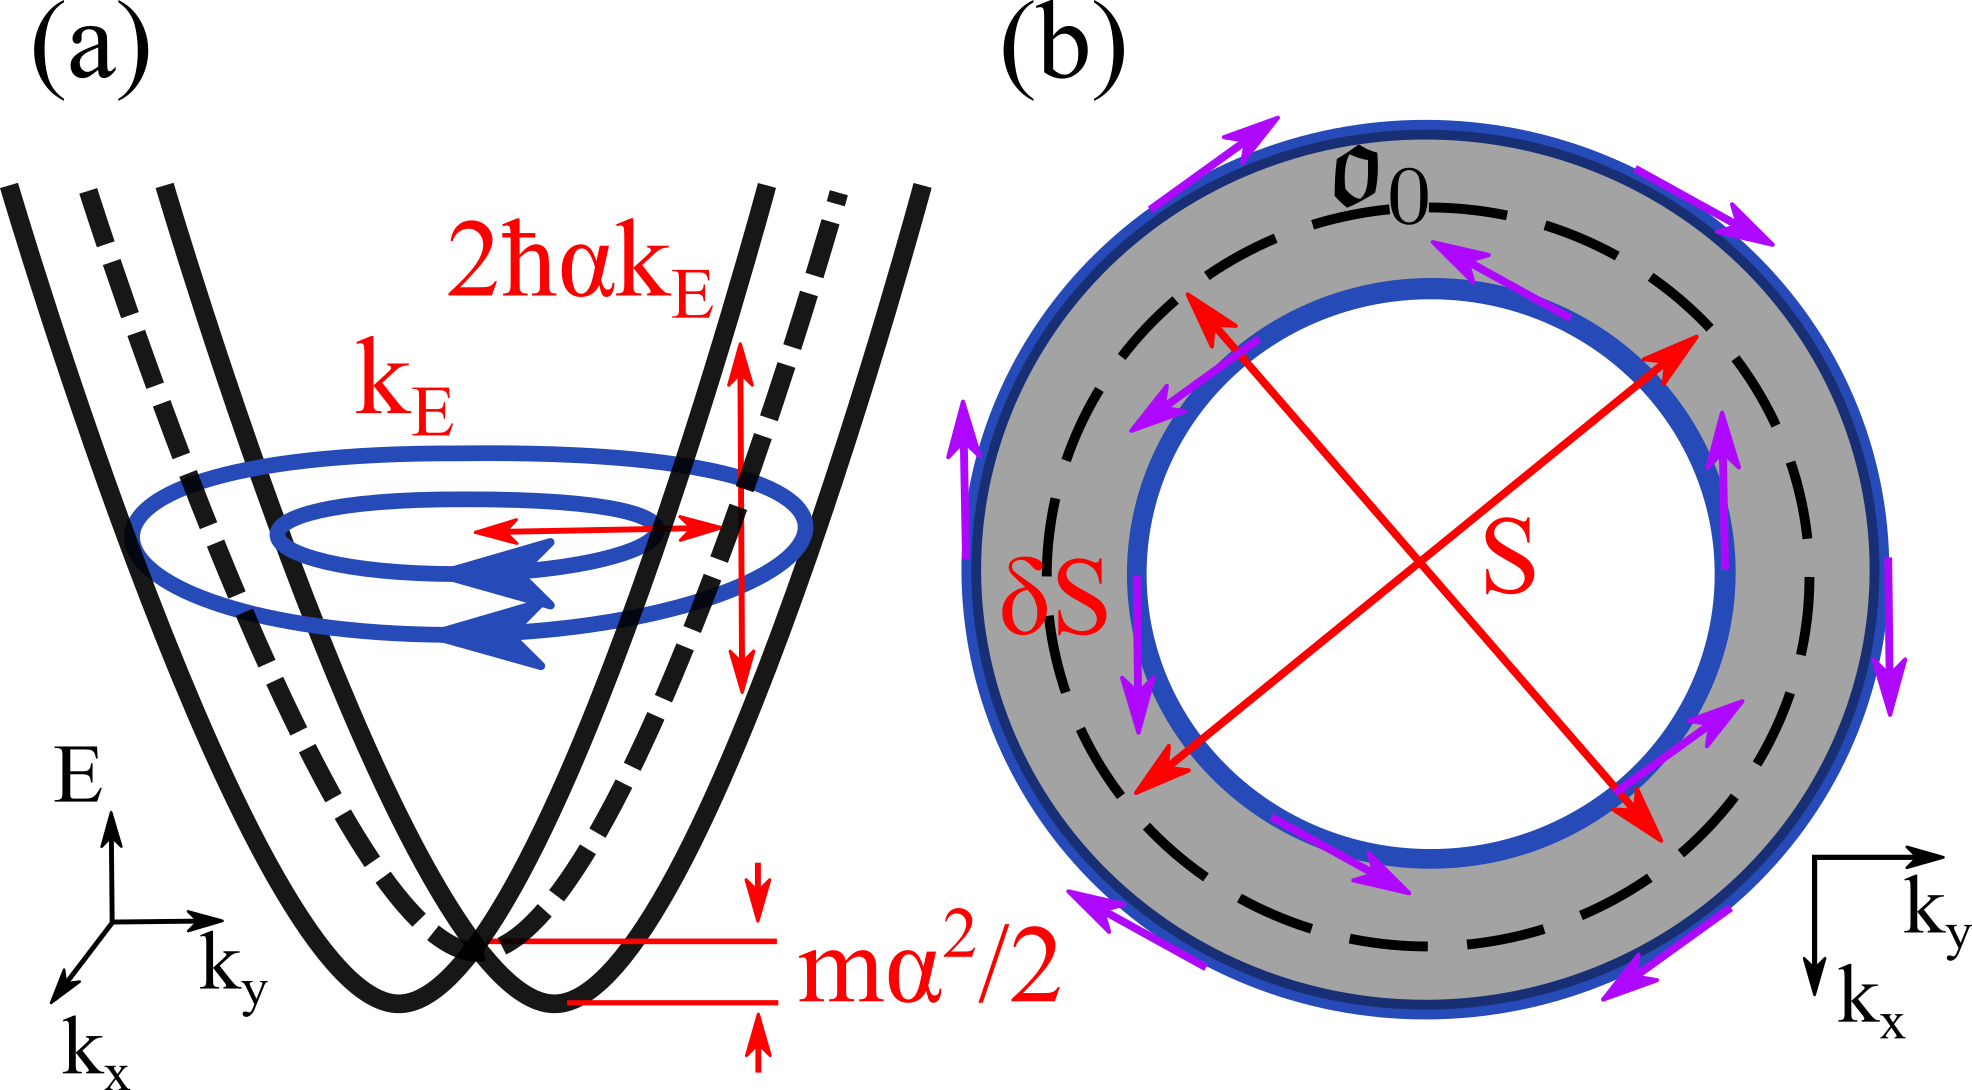
\includegraphics[width=0.8\textwidth]{../figures/orbits.png}
	\centering
	\caption{(a) 实线(虚线)阐释了具有(没有)Rashba自旋轨道耦合的二位电子气的能带色散。图中具有方向的圆代表了磁振子轨道,其中磁场方向为$-z$方向。 (b) 虚的圈$S$标注出了零阶轨道$\frako_0$;$\delta S$是自旋轨道耦合劈裂的轨道的面积之差;紫色的箭头标出了自旋结构。\label{fig:orbits}}
\end{figure}

我们的工作给出了一个适用于近简并能带的推广的量子化条件,这个量子化条件的适用范围包括具有自旋轨道劈裂的能带。我们定义近简并为磁振子面积的差远小于磁振子面积的平均值$|\delta S/S|{\ll}1$。我们提出的量子化条件还依赖于另一个条件:$S$远大于$1/l^2$,这里的$l$是磁长度$l{=}\sqrt{\hbar/eB}$;这个条件也是标准的准经典Onsager-Lifshitz-Roth理论假设。通过引入两个小量$|\delta S/S|$和$1/l^2|S|$,我们的研究推广深化了前人仅仅基于一个小量的准经典理论\cite{kohn_effham,blount_effham,rotheffham,wannier_fredkin,fischbeck_review,Mikitik_quantizationrule,topoferm,100p,gao_zero-field_2017}。

$1/l^2|\delta S|$量化了由塞曼能导致的近简并的轨道的耦合。在$l^2|\delta S|{\gg}1$的情况下,Onsager-Lifshitz{-Roth}量子化条件可以分别作用在两个共心但是不耦合的磁振子轨道。在另外一个极限$l^2|\delta S|{\ll}1$,自旋轨道耦合导致的劈裂可以忽略,我们可以采用已有的严格简并能带的量子化条件\cite{rotheffham,rothmag,topoferm,100p,Mikitik_quantizationrule}。我们的统一的量子化条件给出了介于前述的两个极限情况下的朗道能级的解($l^2|\delta S|{\sim}1$),这种情况下,塞曼能和自旋轨道耦合的能量基本相同;而前人的工作仅仅展示了这两个能量一个远大于另一个的情况下的量子化条件。我们工作给出了在任意对称群的具有自旋轨道耦合的晶体的量子化条件。章节\ref{sec:qtznrules}描述了这个近简并能带的量子化条件,其中我们假设了一个自旋二分之一(或者赝自旋二分之一)的自由度。正如章节\ref{sec:discussion}所述,我们的量子化条件能够涵盖任意带数的近简并能带的朗道量子化。


在章节\ref{sec:Rashba}中,我们利用具有Rashba和Dresselhaus自旋轨道耦合的二维电子气,证明了我们的量子化能级的有效性。如果给具有Rashba自旋轨道耦合的二维电子气加上足够强的面内磁场,能带中的Dirac点不仅仅会移动,而且会倾斜,成为一个第二类的狄拉克点\cite{soluyanov_type-ii_2015, muechler_tilted_2016, bergholtz_topology_2015}。在章节\ref{sec:inplanezeeman}中,我们研究了第二类狄拉克点附近的Landau-Zener隧穿现象。特别的,我们将要证明我们的量子化条件囊括了近简并能带之间的量子隧穿,这个现象被称为带间的磁隧穿\cite{kaganov_coherent_1983,slutskin_dynamics_1968,AALG,100p}。我们将要认真研究一个最近提出的二类狄拉克点附近的完美Klein隧穿的现象\cite{obrien_magnetic_2016},我们发现如果考虑了塞曼效应的话,这个完美隧穿永远不会发生。

\s{sec:llquasideg}应用上述的量子化条件来计算需要多少个参数才能够找到一个朗道能级的(准)简并。如果两个朗道能级属于对称群的不同不可约表示,那么他们的交叉可能是严格的,即使没有这样的情况,朗道能级之间的距离可能仍然非同寻常地小,我们称之为朗道能级准简并【参见\s{sec:relatedegeneracies}】。和Wigner-von Neumann不相交规则\cite{neumann2000behaviour}一致,我们发现没有任何对称性的情况下需要三个参数才能找到朗道能级的准简并。对于有对称性的情况,我们的结果总结在表格\ref{table:codimension-nearlydegen}-\ref{table:codimension-exactlydegen}中。值得一提的是,如果有旋转对称性的存在,那么仅仅需要一个参数就可以调节到朗道能级的准简并。这个参数可以是磁场的大小和方向,也可以是朗道能级的指标。

在\s{sec:quantosc_quasideg}中,我们提出了在低温Shubnikov-de Haas震荡\cite{SdH}中观测到单参数调节的朗道能级的准简并的方法。在\s{sec:quantosc_equidis}中,我们提出了一个推广的Lifshitz-Kosevich公式,使得量子振荡可以直接从我们的量子化条件中得出。特别的,我们提出最低阶量子振荡的相消现象总可以通过调节一个参数获得,从而产生非周期性的拍。

我们在\s{sec:discussion}总结了本章的内容,并展望了未来的研究方向。


\section{量子化条件\label{sec:qtznrules}}

首先让我们大致解释一下这个量子化条件是怎么出现的;我们将这个量子化条件的分步的严格的证明留到附录\ref{app:quantizationruleproof}中。我们要考虑的是一个没有加磁场的时候有着离散平移不变性的哈密顿量: $\hat{H}_0{+}\delta \hat{H}$。前面的这个分解要求$\hat{H}_0$的能带在每一个波矢$\bk$处是$D$重简并的,而$\delta \hat{H}$则作为微扰破除这个$D$重简并。简单起见,我们假设$D{=}2$的自旋简并,$D>2$的情形则留在附录\ref{app:quantizationruleproof}中讨论。一个简单的例子是$\hat{H}_0$是薛定谔哈密顿量,而$\delta \hat{H}$是自旋轨道耦合的哈密顿量;另一个例子是$\hat{H}_0$是具有空间反演的包含自旋轨道耦合的泡利哈密顿量,而$\delta \hat{H}$是一个晶格畸变,轻微破坏了空间反演对称性。

现在让我们加上一个磁场,我们首先考虑忽略$\delta \hat{H}$和塞曼效应的自旋简并的朗道能级。在准经典的描述下,我们对$\hat{H}_0$的低能简并的能带的磁场动力学性质进行考察,这条能带的色散记为$\var(\bk)$。比如说,对于Rashba模型,$\var(\bk){=}\hbar^2 k^2/2m{+}\order(k^4)$。众所周知,朗道量子化是由Peierls修正得到的$\var(\bk){\rightarrow}\var(\bK)$\cite{peierls_substitution},这里的$\boldsymbol{K}{:}{=}\boldsymbol{k}{+}(e/\hbar) \boldsymbol{A}(i\nabla_{\boldsymbol{k}})$,并且$\boldsymbol{A}(\br)$是矢势。我们假设磁场沿着$-z$方向,$[K_x,K_y]{=}i\lmt$。准经典的波函数的解对应着电子在$\var(\bk)$的等能面作回旋运动【见图\ref{fig:orbits}(b)】,这个蕴含着电子运动方向(运动方程为$ \hbar dk_{\alpha}/dt {=} \lmt \epsilon_{\ab}\partial \var/\partial k_{\beta} $,其中 $\epsilon_{xy}{=}{-}\epsilon_{yx}{=}1$)的轨道被称为零阶轨道$\frako_0$。在这个工作中,我们仅仅关注闭合的轨道,闭合的意思指的是轨道不会横穿布里渊区。

朗道能级的量子化条件反映了WKB准经典波函数在轨道$\frako_0$上的单值性\cite{berry_mount_review},换句话说,电子在一个磁振子周期$T_c$中获得的相位是$2\pi$的整数倍:$(l^2S(E){+}\gamma)/2\pi{\in}\Z$。最高阶的相位是是$l^2S{:}{=}{-}l^2\int_{0}^{T_c} k_x \dot{k}_y dt$;$S$同时也可以阐释为具有正负号(对于电子型的轨道是正的)的$\bk$空间$\frako_0$的面积,见图\ref{fig:orbits}(b)。$\gamma$是次低阶的Maslov相位修正\cite{keller1958},这个修正等于$\frako_0$绕的圈数$r$乘以$\pi$,也是其切向量的绕圈数\cite{100p};对于一个能够连续变化为圆的轨道,$r{=}{\pm} 1$。在零阶近似下,所有的朗道能级是自旋简并的,能级间隔是
\e{ \var_c:=\f{2\pi}{l^2|\partial S/\partial E|}:=\f{\hbar^2}{ml^2}:=\f{h}{T_c}. \label{def:cyclotron}}
这里,$\var_c$和$T_c$分别是零阶轨道的磁振子能量和周期,$m$是有效质量。下面开始,朗道能级的简并指的就是自旋简并。



当我们考虑一阶效应的时候,$\delta \hat{H}$和塞曼效应会导致一个一阶的相位修正($\lambda_a$),这个相位修正一般而言对两个不同的自旋态是不同的(我们用$a{=}1,2$标记):
\begin{equation}
l^2S(E)+\lambda_a(E,B)+\gamma=2\pi n,\as  n\in \mathbb{Z},\;a=1,2. \label{eq:rule}
\end{equation}
这表示朗道能级的自旋简并被破除,朗道能级之间的间隔是$\var_c|\lambda_1{-}\lambda_2|/2\pi$。相位修正$\lambda_a$可以看成一个时间周期性的,微扰性的哈密顿量($\calh$)的Floquet准能量\cite{shirley_solution_1965},这个哈密顿量控制着自旋波函数的演化。$\lambda_a$是下面路径有序的指数积分(下面也会直接成为传播子)的本征值$\{e^{i\lambda_a}\}_{a=1}^2$:
\begin{equation}
\A{:}{=}\overline{\exp}\left[-\frac{i}{\hbar}\int_0^{T_c} \calh(\bk(t)) dt\right],
\label{eq:prop}
\end{equation}
这里$\bk(t){\in}\frako_0$是一个时间周期性的函数,由运动方程决定。$\calh$是一个$2\times 2$的矩阵:
\begin{equation}
\calh=\delta \var +B\bigg(M_z -g_s\mu_{B}\f{s_z}{\hbar} + e\epsilon_{\alpha\beta}\mathfrak{X}_{\beta}v_{\alpha}\bigg):=\delta \var+B\calm,\label{eq:H1}
\end{equation}
$\delta \var$是$\delta \hat{H}$在$\hat{H}_0$的简并子空间(也就是前述的两条简并的带)中的投影。出于简单起见,我们假设$\delta \var$的迹是零;如果 $\delta\hat{H}$是一个自旋轨道耦合的哈密顿量,那么$\delta \var$的迹是零是得到保证的。更一般的情况下,我们总可以将$\delta \hat{H}$的投影的有迹的部分吸收到$\var(\bk)$的定义里去。在劈开的能带里(我们将这两个能带标记为${+}$和$-$,其中$+$是外面的轨道,$-$是里面的轨道),$\delta \var$是一个对角的矩阵,其对角元($\delta \var_+,~\delta \var_-{=}{-}\delta \var_+$)和耦合参数相关
\e{-\int_0^{T_c} (\delta \var_+{-}\delta \var_-) \frac{dt}{\hbar} \approx l^2\delta S. \label{spinsplitwkb}}

式\ref{eq:H1}中剩下的项可以看成一个广义的塞曼作用项$B\calm$,这一项正比于$B$,是Peierls-Onsager哈密顿量$\var(\bK)$的一阶修正\cite{rotheffham,blount_effham,kohn_effham}。这个广义的塞曼作用项包括近简并能带的自旋的塞曼作用能($g_s\mu_Bs_z/\hbar$)和轨道磁矩($M_z$)的塞曼作用能\cite{thonhauser_orbital_2005};轨道磁矩可以用布洛赫波$\psi_{n\bk}$之间的速度矩阵元表示出来$\boldsymbol{\Pi}_{mn}=i\langle\psi_m|[\hat{H}_0, \hat{\boldsymbol{r}}]|\psi_n\rangle/\hbar$:

\e{
	[M_z]_{mn}=\f{ie\hbar}{2}\sum_l'\f{\Pi_{x,ml}\Pi_{y,ln}-\Pi_{y,ml}\Pi_{x,ln}}{\epsilon_m-\epsilon_l}. \label{eq:orbitalmoment}
}
这里,对$l$的求和不包括这两条近简并的能带。最后,广义的塞曼作用项还包括一个几何相位的贡献,这一个贡献可以用$2\times 2$的非阿贝尔的贝里联络\cite{berry_quantal_1984,wilczek_appearance_1984}和零阶的能带速度表达出来
\e{\mathfrak{X}_{\beta,mn}{=}i\braket{u_m}{\partial u_n/\partial k_{\beta}},  \;\;\;v_{\alpha}:= \f{1}{\hbar}\p{\var}{k_{\alpha}},\label{berryconn}}
这里$\{u_n\}_{n=1}^2$是布洛赫波的周期性部分。

式\ref{eq:rule}至\ref{berryconn}能够让我们将$\lambda_{1,2}$计算到$1/l^2|S|$和$|\delta S/S|$的最低阶,这些式子对任意有限的$l^2|\delta S|$和$|B\calm|/\delta \var_{\pm}$都是有效的。值得指出的是,我们提出的量子化条件相对于近简并能带构成的子空间内的幺正变换是不变的(见附录\ref{app:quantizationruleproof})。在下面的讨论中,如果可能的话,有的时候采用一个和$\bk$无关的基来表达$\calh$更加方便,这种情况下,非阿贝尔的贝里联络这组基下面为零。

\subsection{在两种极限情况下恢复到Onsager-Lifshitz量子化条件}\label{sec:recoveronsager}

现在,我们用近简并的能带(用$\pm$标识)作基,讨论一下$\delta \var$和$B\calm$相互之间的大小关系。我们将要证明,在其中一个远大于另外一个的情况下,我们提出的量子化条件会恢复到已有的针对独立轨道或者严格简并轨道的Onsager-Lifshitz-Roth量子化条件。

\noi{i} 如果$|\var_+{-}\var_-|$在$\frako_0$的每一个点都远大于$B|\calm_{+-}|$。在这样的情况下,电子在磁场下将会进行绝热(也就是维持在同一个能带的)运动\cite{nenciu_review},此时两个轨道可以看成非简并并且独立的。在$B{\rightarrow} 0$的情况下,如果两条近简并的能带没有交上的话,电子的运动始终会退化为绝热运动。(有的时候近简并的能带会交上,一个例子就是二类狄拉克点,这个例子将在小节\ref{sec:inplanezeeman}和小节\ref{sec:rotsymmbreakdown}中讨论)在这样的情况下,我们可以忽略带间跃迁的矩阵元$B\calm_{+-}$,此时$\cala$成为一个对角的矩阵,对角元$e^{i\lambda_{\pm}}$为
\e{\lambda_{\sma{\pm}} = -\int_0^{T_c}\calh_{\sma{\pm\pm}}\f{dt}{\hbar}=\pm \f{1}{2}l^2\delta S - B\int_0^{T_c}\calm_{\sma{\pm\pm}}\f{dt}{\hbar}.  \label{phaseindependentorbit}}
式\ref{eq:rule},以及式\ref{phaseindependentorbit},和前人的针对独立,非简并的面积为$S{\pm}\delta S$的两个轨道的Onsager-Lifshitz量子化条件是一致的\cite{Onsager,lifshitz_kosevich,lifshitz_kosevich_jetp}。这个独立轨道的量子化条件包含了首先由Roth\cite{rothmag}提出的相位修正。如果我们微扰地加进$B\calm_{\sma{+-}}$,$\lambda_{\pm}$ (参见 式\ref{phaseindependentorbit})可以表达为$B$地洛朗级数,并且最低阶项时$1/B$;这一点将会在下面地样例讨论(参见式 \ref{lambdasmallB})中设计,并且会被用来解释量子振荡的多种现象(参见节\ref{sec:qo})。


\noi{ii} 让我们现在讨论广义的塞曼能$B\calm$远大于$(\delta \var_+{-}\delta\var_-)$的情况。式\ref{eq:rule}至\ref{berryconn}以及$\calh{\approx}B\calm$,和我们之前的工作中\cite{topoferm,100p}得到的任意对称性的简并轨道的量子化条件是一致的。


由式\ref{eq:rule}至\ref{berryconn}总结出来的量子化条件,是本章的理论性的进展,本章下面的内容主要关注这个量子化条件会带来什么样的物理现象。我们首先要在绝热近似失效的时候(也就是$\delta \epsilon$和$B\calm$的大小相互竞争的时候)证明我们的量子化条件的有效性,这包括两种情况:(i)如果自旋劈裂的轨道在连续旋转变换下不变(比如说Rashba二维电子气模型),那么绝热近似在整个轨道都会失效【参见节\ref{sec:Rashba}】。(ii)如果自旋劈裂的轨道是不对称的,绝热近似有可能在某一个孤立的点失效,一个简单的例子就是能带在第二类狄拉克点处相交【参见节\ref{sec:inplanezeeman}】。在节\ref{sec:llquasideg}中,我们将要讨论多少个实的参数才能够调节得到$\lambda_1{=}\lambda_2$(mod $2\pi$),这个式子等价于朗道能级的近简并。


\section{案例研究:任意方向磁场中的Rashba二维电子气}

\subsection{面外磁场中的Rashba二维电子气}\label{sec:Rashba}

在这一节里,我们将要将我们的量子化条件应用于Rashba模型(参见式\ref{eq:Rashba-Hamiltonian}),这个模型的朗道能级有着严格解,可以和我们的量子化条件做对比\cite{bychkov_oscillatory_1984}。

出于简单起见,我们认为式\ref{eq:Rashba-Hamiltonian}中的泡利矩阵对应的就是自旋:$s_i{=}\hbar \sigma_i/2$。我们来计算半径为$k$的磁振子轨道$\frako_0$上的有效哈密顿量$\calh(\bk)$。用Rashba哈密顿量$H_R$【参见式\ref{eq:Rashba-Hamiltonian}】的能带布洛赫波(也就是$H_R$的本征态)作基
\e{\calh(\bk)=-\hbar\alpha k\tau_z{+}\f{g_{s\perp}}{2}\mu_{\sma{B}}B\tau_x {-} \f{eB\hbar}{2m} (\tau_x-I) \epsilon_{\alpha\beta} k_{\alpha}\nabla_{\beta}\theta,\label{rashbaeffham}}
这里$\tau_i$是一套新的泡利矩阵,$\tau_z{=}{+} 1$ 和 ${-}1$ 分别对应的是外轨道和内轨道。 $e^{i\theta_{\bk}}{=}(ik_x{-}k_y)/k$是面内的$H_R$的自旋劈裂场$(-\hbar\alpha k_y,\hbar\alpha k_x,0)$的角度【参见式 \ref{eq:Rashba-Hamiltonian}】,这个自旋劈裂场在$\frako_0$上转了一圈;由于我们基的自旋平行(或者反平行)于自旋劈裂场,因此也转了一圈【参见图\ref{fig:orbits}(b)】。上式中正比如自旋旋转速度($\nabk \theta$)的项来自于非阿贝尔的贝里联络。$\calh$的第一项对应于自旋轨道耦合引起的劈裂;其余项可以认为是磁场导致的能带变形。轨道磁矩$B M_z$一般而言会混合近简并的两个带和其余的所有能带,在这里这个效应被吸收在有效的$g$因子中$g_{s\perp}$。众所周知,塞曼效应一般会让自旋朝向磁场$\bB$的方向;令人惊异的是,非阿贝尔的贝里相位在这里也有一个自旋极化的效应,但是和塞曼效应方向相反。这两个效应在自由电子的时候完全抵消($g_{s\perp}=2$以及 $m$等于自由电子质量$m_0$),这个抵消一般不发生在能带电子上。

由于$H_R$的连续旋转对称性的存在,$\nabk \theta$的大小是$1/k$,并且和$\frako_0$相切;因此,$\calh$在$\frako_0$上是一个常数,而传播子则化简为不需要路径有序的$\cala{=}e^{{-}i\calh T_c/\hbar}$,因此量子化条件的相位修正仅仅是$\calh$的本征值乘以$T_c$:
\begin{equation}
\lambda_{\pm}=\pm\f1{2}\sqrt{({l^2\delta S})^2+\pi^2(g_{s\perp}m/m_0-2)^2}+\pi. \label{eq:Rashba-lambda}
\end{equation}
这是一个面积差$\delta S$(参见式\ref{deltaSvsS})和有效质量$m$的函数。多出来的$\pi$来自于单带的贝里相位,体现在$\theta_{\bk}$绕了${\pm}2\pi$。两个在根号下面的量来自于自旋轨道耦合导致的轨道劈裂$\delta \var$以及(在零场的能带基下的)$B\calm$的带间矩阵元。

在弱耦合极限下,$l^2\delta S \gg \pi|g_{s\perp} m/m_0{-}2|$,我们可以将式\ref{eq:Rashba-lambda}展开为$B$的洛朗级数:
\e{\lambda_{\pm}= \pm \f{l^2\delta S}{2} +\pi \pm \f{\pi^2}{4}\f{(g_{s\perp}m/m_0-2)^2}{l^2\delta S} + O(B^2). \label{lambdasmallB}}
式\ref{lambdasmallB}的右手边前两项,也可以从标准的针对独立轨道的Onsager-Lifshitz量子化条件导出,其中$\pi$来自于贝里相位的修正。更高阶的项则来自于磁场导致的能带之间的混合。Mineev在Rashba模型下得到了式\ref{lambdasmallB}中的一部分\cite{mineev_haas--van_2005};由于没有考虑带间的贝里联络,他漏掉了$(g_{s\perp}m/m_0-2)$中的第二项(参见式\ref{lambdasmallB})。

在强耦合极限,也就是$l^2\delta S {\ll}\pi(g_{s\perp}m/m_0{-}2)$的情况下,$\lambda_{\pm}{\approx}{\pm}\pi g_{s\perp}m/2m_0$ mod $2\pi$,这对应着没有自旋轨道耦合的情况下,朗道能级劈裂了$g_{s}\mu_BB$。

我们的量子化条件【式\ref{eq:rule}和\ref{eq:Rashba-lambda}】可以和已知的Peierls替换过的哈密顿量(加上自旋塞曼效应)的精确解进行比对。精确解\cite{bychkov_oscillatory_1984}可以通过下式得出:
\e{
	&n_{\pm}=\frac{l^2S}{2\pi}+\frac{l^2\delta S}{16\pi}\f{\delta S}{S}\lin 
	&\pm\f1{2}\sqrt{\bigg(\frac{l^2\delta S}{8\pi}\f{\delta S}{S}\bigg)^2+(l^2\delta S)^2+\pi^2\bigg(\f{g_{s\perp}m}{m_0}-2\bigg)^2},\label{eq:Rashba-exact}}
这里的$\delta S(E)$和$S(E)$的形式参见式\ref{deltaSvsS};$n_{+}{\ge} 1$和$n_-{\ge} 0$是整数的朗道能级的标号,$\pm$代表两套朗道能级。在近简并的($\delta S/S\ll 1$)准经典的($1/l^2S \ll 1$)情况下,在$l^2\delta S$是有限的时候,式\ref{eq:Rashba-exact}里面的$\delta S/S$项可以忽略,于是式\ref{eq:Rashba-exact}就退化为我们的量子化条件,其中$\lambda_{\pm}$由是\ref{eq:Rashba-lambda}给出。


我们进一步给$H_R$加上Dresselhaus自旋轨道耦合,在这样的情况下,据我们所知,朗道能级的严格解析解是不存在的。这种情况下,我们可以通过数值对角化来验证我们的量子化条件的可靠性,这一部分内容在附录\ref{app:approximatevsexact}中。

\subsection{磁隧穿的案例研究:倾斜磁场中的Rashba二维电子气}\label{sec:inplanezeeman}

我们的下一个案例研究是一个(接近)相交的二类狄拉克点\cite{soluyanov_type-ii_2015,muechler_tilted_2016}。二类狄拉克点是传统狄拉克点的一个变种,其区别在于二类狄拉克点的能带色散不是对称的。在二类狄拉克点附近的量子隧穿数学上和Landau-Zener隧穿是一致的,仅仅是电场力变成了洛伦兹力\cite{AALG,obrien_magnetic_2016,kane_blount}。这里,我们将要证明Landau-Zener动力学很自然的可以从我们的量子化条件得出【式\ref{eq:rule}到式\ref{eq:H1}】我们将要研究电子的运动会怎么受到塞曼效应的影响。特别地,我们将会展示O'Brien等人预言的\cite{obrien_magnetic_2016}完美的Klein透射在考虑进塞曼效应之后,并不是真正地完美。

我们再次从Rashba模型出发【参见式\ref{eq:Rashba-Hamiltonian}】,它有一个旋转对称的狄拉克点。要将这个狄拉克点变成二类的,我们引入一个面内的磁场$B_\parallel$(平行于$y$方向)导致的塞曼项:
\e{ 
	H_{RZ}=\f{{\hbar^2}k^{2}}{2m}+\delta \var; \;\;\;\delta \var=d_x\sigma_x+d_y\sigma_y,\lin
	(d_x,d_y):=(-\hbar\alpha k_y,\hbar\alpha k_x+\zpar),\;\;\;\zpar:= g_{s\parallel} \mu_B B_{\parallel}/2.
	\label{eq:RZ-Hamiltonian}}
尽管这一项同时破坏了时间反演($T$)和二重旋转($\rot_2$),他们的乘积($\rot_2 T$)还是哈密顿量的对称性,这一点体现在 $\sigma_x H^*_{RZ}(\bk)\sigma_x{=}H_{RZ}(\bk)$, 并且让每个$\bk$的自旋严格躺在面内。二维情况下,在这个对称群中,狄拉克点可以移动,但是不能够打开能隙。面内的塞曼场不仅挪动了狄拉克点的位置到
\begin{eqnarray}
\bar{k}_x & = & -\frac{\zpar}{\hbar\alpha},\;\bar{k}_y=0,\;\epsilon_{0}=\frac{\zpar^{2}}{2m\alpha^2},\label{whereisdiracpoint}
\end{eqnarray}
而且将狄拉克点的能带倾斜了过来。如果我们在狄拉克点附近线性化这个哈密顿量,我们就可以看到这个倾斜
\e{
	H & =\hbar\alpha\left[\left(\sigma_y-\frac{\zpar}{m\alpha^2}\right)\delta k_{x}-\sigma_{x}\delta k_{y}\right]+\epsilon_{0}.}
当$|\zpar|>|m\alpha^2|$的时候,狄拉克锥在$x$方向倾斜角度超过了90度,进而导致等能线的Lifshitz相变。在线性近似下,等能线从圆形变成了双曲线,这一点体现在图\ref{fig:RZ}(a)中。一个倾斜超过九十度的狄拉克锥就是第二类的狄拉克锥。我们的案例研究就是要研究两个电子口袋连接在一起的第二类狄拉克点(参见图\ref{fig:RZ}(a,b)),这个案例研究和前人的不同\cite{obrien_magnetic_2016,AALG},前人研究的第二类狄拉克点是电子和空穴口袋之间相交得到的。

\begin{figure}
	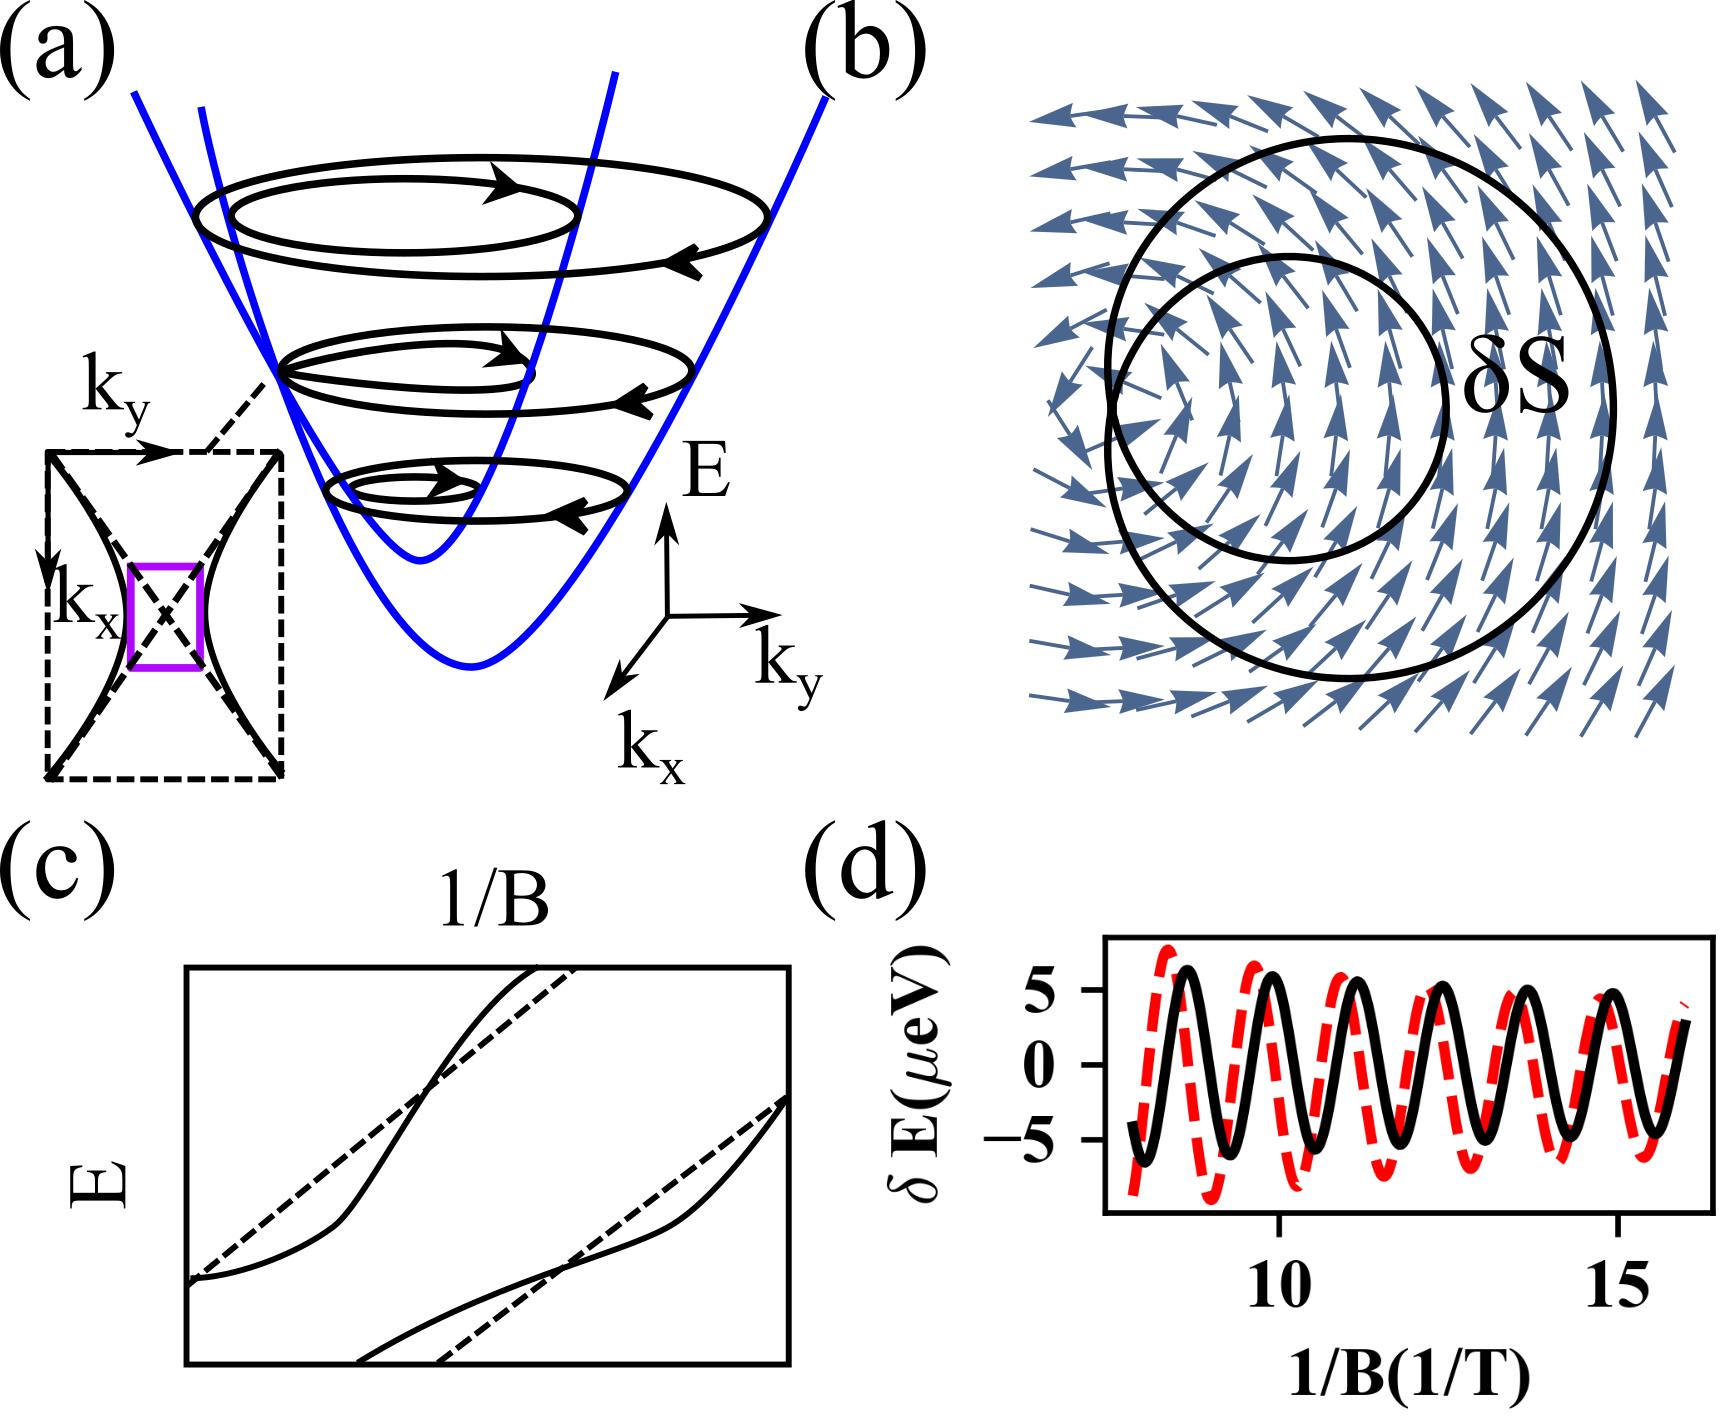
\includegraphics[width=0.8\columnwidth]{../figures/RZ.png}
	\centering
	\caption{(a)展示了Rashba二维电子气在倾斜磁场中的磁振子轨道。内嵌的图展示了第二类狄拉克点的放大图。(b)展示了能量正好在第二类狄拉克点的时候的磁振子轨道。一个能够Klein透射的电子将会沿着这个莫比乌斯环形的轨道运动。这个图片的背景是自旋劈裂场的方向($d_x,d_y$),自旋劈裂场导致了原先的能带$\delta\var$的能量劈裂(参见式\ref{eq:RZ-Hamiltonian}。内(外)圈的波函数的自旋是平行于(反平行于)自旋劈裂场的。(c)在弱耦合情况下,演示了在第二类狄拉克点附近的朗道能级。虚线是莫比乌斯轨道的Onsager-Lifshitz-Roth量子化能级(参见式\ref{trefoilrule}),实线则包含了隧穿导致的的一阶修正(参见式\ref{RZfirstorderE}) (d) 黑色的实线是$\delta E_n$(参见式\ref{RZfirstorderE}),也就是由于不是完美Klein透射导致的能量修正;作为对比,红色的虚线是数值严格对角化得到的相应的能量修正。这个图采用了最接近0.45eV的朗道能级,并且采用了偶数$n$;在我们采用的参数下 ($m{=}0.076m_0$, $\alpha{=} 1.5\times10^{5}$cm/s, $Z_\parallel {=}$1meV 以及 $g_{s\perp}=2$),二类狄拉克点在 0.5eV处。 
	\label{fig:RZ}}
\end{figure}

在面内的磁场以外,我们再加入一个面外的磁场$B_{\perp}$,其磁长度为$\lper{=}\sqrt{\hbar/eB_{\perp}}$,磁振子能量为$\var^{\sma{\perp}}_c{:}{=}\hbar^2/m\lper^2{:}{=}\hbar \omega_c^{\sma{\perp}}{:}{=}h/T_c^{\sma{\perp}}$,自旋塞曼效应为$\zper{:}{=}{g_{s\perp}}\mu_B B_{\perp}/2$。我们在这里假设$1/\lper^2S{\ll}1$,这里$S$是零阶轨道(有效质量为$m$半径为$k_E{=}\sqrt{2mE}/\hbar$)。对于远高于$m\alpha^2$和 $\zpar$的能量,近简并条件($\delta S/S{\ll}1$)是满足的,这里$\delta S$是自旋轨道和耦合和面内的塞曼场导致的磁振子轨道的面积差【参见图\ref{fig:RZ}(b)】。由于$1/\lper^2S$和$\delta S/S$很小($\lper^2\delta S$是有限的),我们的量子化条件(参见式\ref{eq:rule}至式\ref{eq:H1})可以应用于这个模型,其有效哈密顿量为
\begin{equation}
\calh(t)=\hbar\alpha(k_{x}\sigma_{y}-k_{y}\sigma_{x})+Z_\parallel\sigma_{y}-Z_\perp\sigma_{z}.\label{calHRZ}
\end{equation}
这里,$t$是一个参数化零阶轨道的参数$\bk(t){=}({-}k_E \cos \omega_c^{\sma{\perp}} t, k_E \sin \omega_c^{\sma{\perp}} t)$,在式\ref{calHRZ}所采用的动量无关的自旋基矢下,式\ref{eq:H1}中的非阿贝尔的贝里联络$\mathfrak{X}$为零,因此广义的塞曼作用$B_{\sma{\perp}}\calm$退化为对自旋的塞曼作用$Z_\perp\sigma_{z}$。

正如节\ref{sec:qtznrules}所述,如果两个轨道在一个二类狄拉克点相交,那么绝热极限是不存在的。为了研究这个绝热近似是怎么失效的,我们来研究靠近狄拉克点能量($\epsilon_0$)的朗道能级。我们首先关注除了狄拉克点之外,零级轨道$\frako_0$上处处弱耦合的情况。这个条件等价于能量劈裂(参见式\ref{eq:RZ-Hamiltonian})$|\delta \var_+{-}\delta \var_-|$远大于$B_\perp|\calm_{\sma{+-}}|$,也等价于$\hbar\alpha k_{\sma{E}}{\gg}\var_c^\perp$。在狄拉克点附近(此时定义$t{=}0$),研究电子的运动可以采取线性化$\H$的方法,得到
\e{
	\calh = -\hbar\alpha k_{E}\omega^{\sma{\perp}}_c t\,\sigma_x+(Z_\parallel-\alpha k_{E})\sigma_y-Z_\perp\sigma_z,\label{effhamIIDirac}
}
$\sigma_x$的本征矢就是两个非绝热的能级,其特征斜率为$v_d{:}{=}\hbar\alpha k_E\omega^{\sma{\perp}}_c$;在$t{=}0$的时候,由于$\sigma_{y,z}$的存在,两个非绝热能级会耦合,并且打开一个能隙。一般而言,一个非绝热能级隧穿到另一个非绝热能级的概率是$\rho^2{=}\exp(-2\pi\barmu)$,这里的$\barmu{=}{E_g}^2/{2v_d \hbar}$,而$E_g$是能隙\cite{wittig_landauzener_2005,lifshitz_e.m._quantum_1991};在这种情况下
\e{\barmu=\frac{Z_\perp^2+(Z_\parallel-\alpha k_{E})^2}{2\hbar\alpha k_{E}\var^{\sma{\perp}}_c}, \label{mu1}}
这里$2\hbar\alpha k_E$是能量$E$处的自旋轨道劈裂【参见图\ref{fig:orbits}(a)】。在没有考虑面外的自旋塞曼劈裂的情况下($Z_\perp{=}0$),$\bar{\mu}$在狄拉克点的能量为零 -- 也就是会得到一个概率为1的Klein隧穿,这一点是由文献\onlinecite{obrien_magnetic_2016}在另外一个第二类狄拉克点模型中第一次提出的。但是,如果考虑进$Z_\perp$的话,$\bar{\mu}$永远都不会为零,其最小值为$\bar{\mu}_{\sma{\text{min}}}{:}{=} (g_{s\perp} m/m_0)(Z_\perp/4\hbar\alpha k_{E})$,这个式子也是无量纲的有效质量乘以面外塞曼劈裂除以自旋轨道劈裂。这个最小值对于半导体异质结或者重费米子体系可能比较显著(比如对InAs异质结而言,$g_{s\perp}m/m_0{\sim} 1$)。


如果要得到朗道能级,我们不仅仅需要知道隧穿的概率,还需要知道隧穿过去的波函数的相位。这些信息包含在一个散射矩阵中\cite{AALG,kaganov_coherent_1983}
\e{\mathbb{S}=\matrixtwo{\tau e^{i\barphi}}{-\rho}{\rho}{\tau e^{-i\barphi}},\;\rho=e^{-\pi\barmu},\;\tau=\sqrt{1-\rho^{2}}\label{scattmat}}
这是一个将两分量的WKB准经典波函数在Dirac点附近联系在一起的一个矩阵。这个公式是在塞曼修正过的能带作为基写出来的(也就是式\ref{calHRZ}的本征态);$\mathbb{S}$的对角项(非对角项)对应着带内跃迁(带间跃迁)。带内跃迁的相位是 $\barphi{:}{=}\barmu{-}\barmu\ln\barmu{+}\text{arg}[\Gamma(i\barmu)]{+}\pi/4$其中$\Gamma$是$\Gamma$函数。

远离二类狄拉克点的地方,电子将会以绝热演化(保持在同一个能带)的方式运动。将Landau-Zener隧穿和绝热演化结合起来,我们就可以得到下面的传播子:
\e{{\A}= \matrixtwo{\tau e^{i\bar{\varphi}}}{-\rho}{\rho}{\tau e^{-i\bar{\varphi}}} \diagmatrix{e^{i\tilde{\lambda}_-}}{e^{i\tilde{\lambda}_+}}. \label{propinplanezeeman}}
绝热演化的相位$\tilde{\lambda}_{\pm}$是动力学相位${\pm} l^2 \delta S/2$和外轨道($+$)和内轨道($+$)的贝里相位$\phi^B_\pm$之和。在远高于狄拉克点的地方($|E{-}\epsilon_0|{\gg}|Z_{\perp}|$),Zeeman效应可以忽略,无论是外轨道还是内轨道都包含了狄拉克点,因此$\phi_{\pm}^B{\approx}{\pm}\pi$;在远低于狄拉克点的时候,两个轨道都没有包含狄拉克点,因此$\phi_{\pm}^B{\approx}0$;在狄拉克点附近的时候, $\phi_{+}^B$($\phi_{-}^B$)随着能量连续减少(增加),这一点可以从图\ref{fig:blochsphere}中的布洛赫球上看出来。

\begin{figure}
	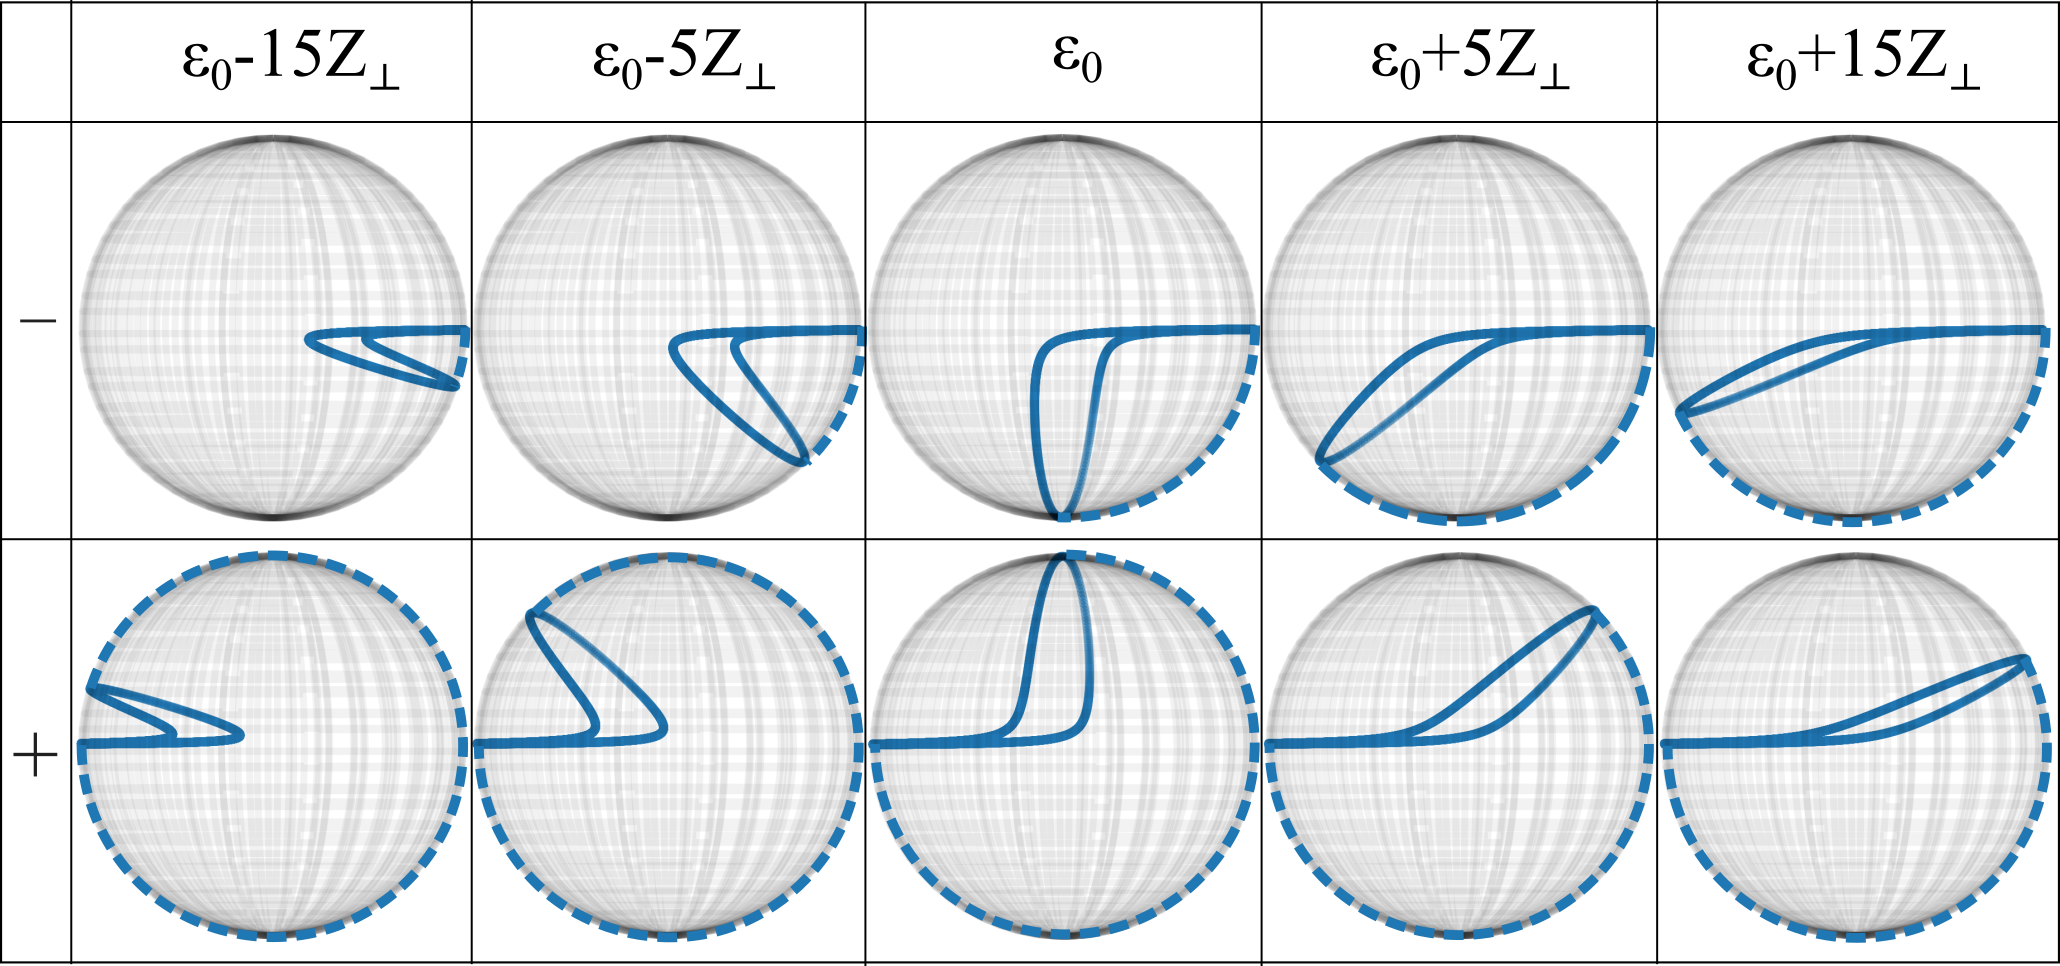
\includegraphics[width=0.8\textwidth]{../figures/blochsphere.png}
	\centering
	\caption{在狄拉克点能量($\epsilon_0$)附近的几个能量出,内轨道(符号是$-$,上排)和外轨道(符号是是$+$,下排)的贝里相位$\phi_{\pm}^B$的立体角表示(参见式\ref{whereisdiracpoint})。在这里,有效哈密顿量(参见式\ref{calHRZ})可以用泡利矩阵分解($\calh{=}\sum_j\calh_j\sigma_j$),这个分解定义了一个三维向量$\boldsymbol{\calh}{=}({-}\alpha k_y$,$\alpha k_x{+}Z_\parallel,{-}Z_\perp)$。$\phi_{\pm}^B$等于${\mp} \boldsymbol{\calh}(\bk)$在$\bk$变化的时候(蓝色的实线)张成的立体角的一半\cite{berry_quantal_1984};立体角的方向由蓝色的虚线表示出来。面外的塞曼场将$\boldsymbol{\calh}$朝向偏出$x-y$平面,但是这个效应仅仅在磁振子轨道的一小部分$(\sim Z_{\perp}/\hbar \alpha k_E)$有明显的贡献。\label{fig:blochsphere}}
\end{figure}

我们的量子化条件(参见式\ref{eq:rule}至\ref{eq:H1}),加上式\ref{propinplanezeeman}中的$\A$的形式,可以简洁地表达为
\e{
	\text{cos}\left[\frac{\Omega_{-}+\Omega_{+}}{2}\right]=\tau\,\text{cos}\left[\frac{\Omega_{-}-\Omega_{+}}{2}+\bar{\varphi}\right], \lin
	\ins{其中}\;\Omega_{\pm}=l^2 (S\pm \delta S/2)+\phi_{\pm}^B +\gamma_{\pm}, \label{coscos}
}
$\Omega_{\pm}$是电子在绝热演化穿过$\pm$标志的内外轨道的时候获得的相位;Maslov修正对于圆轨道是$\gamma_{\pm}{=}\pi$。在电子口袋和空穴口袋相交的第二类狄拉克点模型中,也有类似于式\ref{coscos}的量子化条件\cite{AALG}。

在$\bar{\mu}{\rightarrow} \infty$的极限下,Landau-Zener隧穿可以忽略($\tau{\rightarrow}1,\bar{\varphi}{\rightarrow}0$),这个时候式\ref{coscos}简化为两个独立轨道的Onsager-Lifshitz-Roth量子化条件$\Omega_{\pm}/2\pi{\in}\Z$。

对于不为零的磁场,$0{<}\tau{<}1$意味着两个谐频$(\Omega_+{\pm}\Omega_-)$在式\ref{coscos}中会相互竞争,得到一个准随机的朗道能谱\cite{kaganov_coherent_1983}。准随机指的是能谱在磁振子能量的尺度是乱的,但是在更大的尺度上相互关联。要理解这一点,我们将$\tau$看成小量,采用微扰法来分析狄拉克点附近的朗道能级。零阶的情况下,式\ref{coscos}化简为
\e{2l^2S(E_n^0)+\pi = 2\pi n \rightarrow \{E_n^0(B)\}_{n\in\Z}.\label{trefoilrule}}
在导出上面的式子的过程中,我们用到了$\phi^B_-{+}\phi^B_+{=}0$,这一点对于任意的二带模型都是成立的;在图\ref{fig:blochsphere}中,这一点体现在同一能量的两个立体角加和是$4\pi$。式\ref{trefoilrule}可以认为是莫比乌斯轨道【参见\fig{fig:RZ}(b)】的量子化条件,其面积是$2S{=}4\pi m E{/\hbar^2}$;对应的朗道能级(在图\ref{fig:RZ}(c)中画成了实线)相对于$E{\rightarrow}E{+}\pi/l^2(\partial S/\partial E)$和$l^2{\rightarrow}l^2{+}\pi/S$是周期性的。式\ref{trefoilrule}中的$\pi$的相位修正来自于波函数在整个莫比乌斯轨道上的$2\pi$的相位旋转导致的贝里相位,这一点展示在图\ref{fig:RZ}(b)。由于Maslov修正等于$\pi$乘以轨道的绕转数,在这个例子里Maslov修正为$2\pi$。

总结一下,$E_n^0(B)$(参见式\ref{trefoilrule})在小的能量尺度也是周期性的,这个周期性和莫比乌斯轨道的面积有关。如果考虑到Klein透射是非完美的,那么这个小能量尺度上的周期性就会丢失,但是大能量尺度上的关联始终存在(这个大能量尺度对应着自旋劈裂的轨道之间的面积差$\delta S$),这一点可以从关于$\tau$的一阶修正看出来:
\e{&\delta E_n(B) = \f{(-1)^n}{2\pi} \tau \var_c^\perp \cos\bigg(\f{l^2\delta S}{{2}}+\f{\phi_+^B-\phi_-^B}{2}-\bar{\varphi}\bigg) \lin
	&\approx \f{(-1)^{n+1}m\alpha^2(E-\epsilon_0)(\var_c^{\perp})^{1/2}}{2\sqrt{\pi}\hbar^2
		Z_{\parallel}^{3/2}}\cos\bigg(\f{l^2\delta S}{{2}}-\bar{\varphi}\bigg),\label{RZfirstorderE}}
上式右侧应该在$E{=}E_n^0(B)$计算。第二行开始,我们做了近似$Z_{\perp}{\rightarrow}0$,这个近似在 $g_{s\perp}m{\ll}m_0$的时候是合理的。对于两个相邻的朗道能级,我们在图\ref{fig:RZ}(c)里画出了$E_n^{(0)}+\delta E_n$。图\ref{fig:RZ}(d)中式\ref{RZfirstorderE}和数值对角化的比较证明了式\ref{RZfirstorderE}的正确性。

\section{朗道能级的准简并}\label{sec:llquasideg}

\begin{figure}
	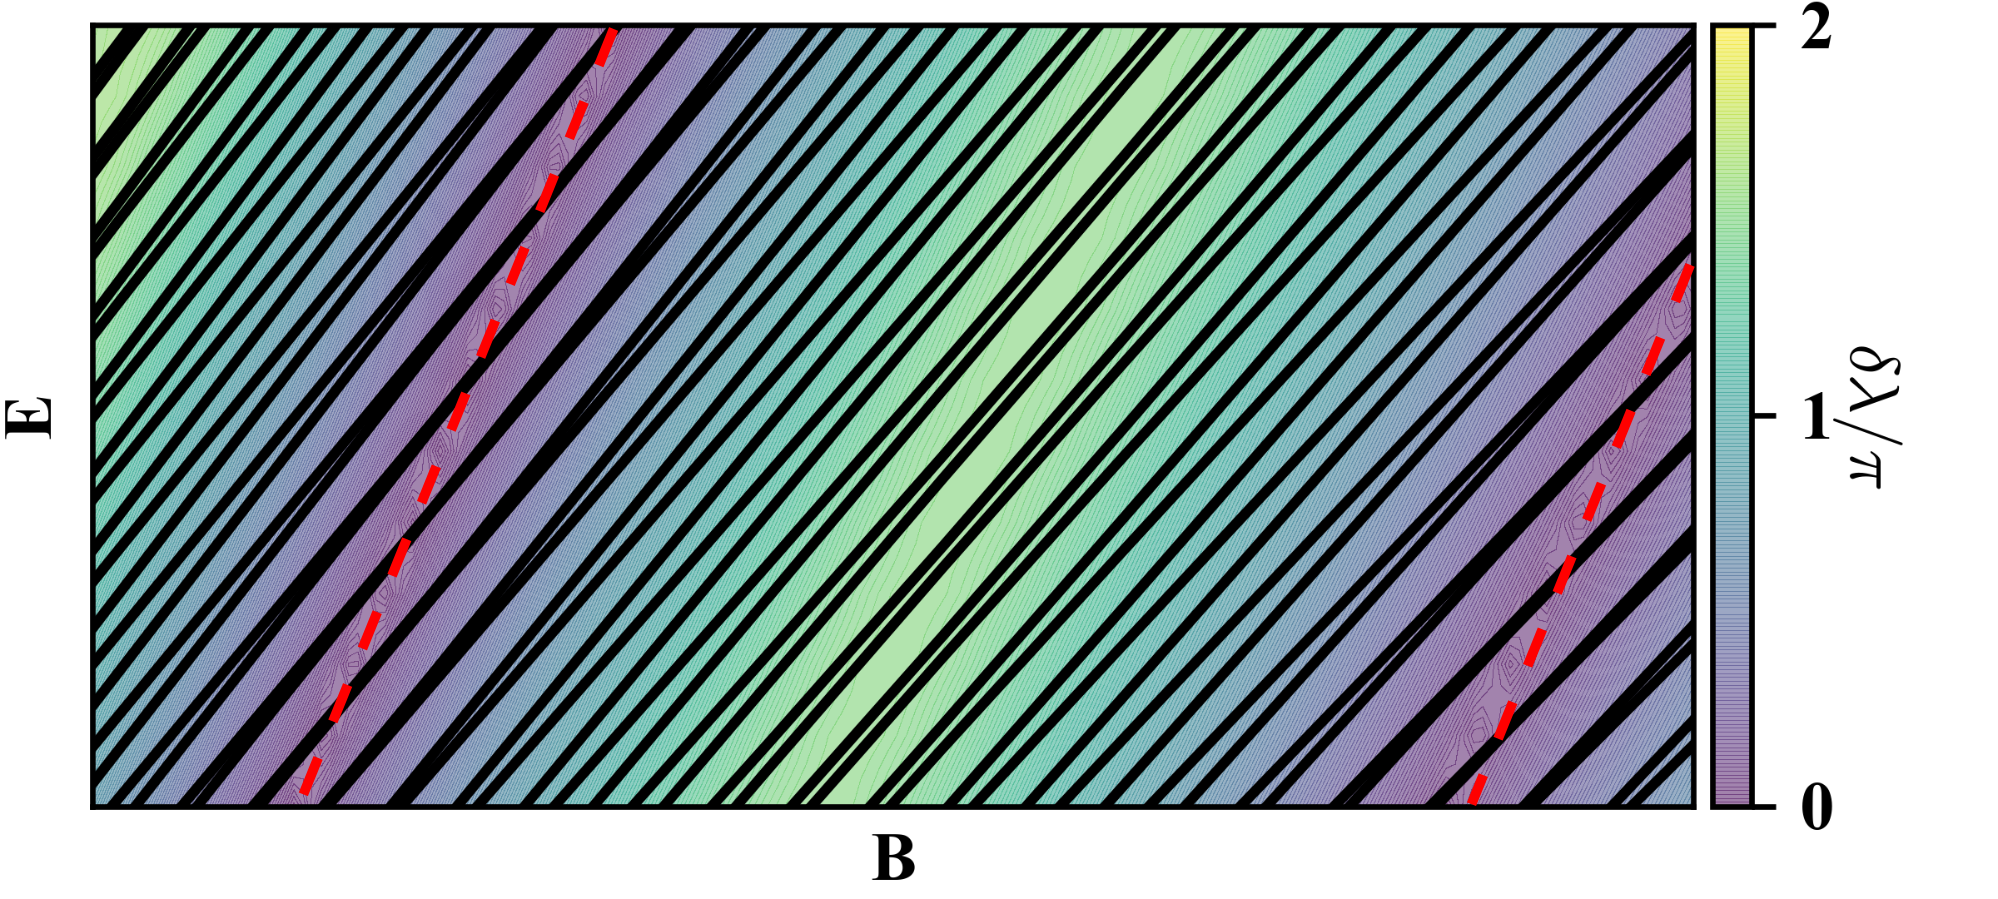
\includegraphics[width=1.0\textwidth]{../figures/LL.png}
	\centering
	\caption{近简并能带中,朗道能级(实线)相对于$B$的色散的一个示意图。背景中的颜色表示的是$\delta\lambda$。当$\delta\lambda\equiv 0\equiv 2\pi$时(用红色的虚线标记),朗道能级就会出现准简并。\label{fig:LL}}
\end{figure}

从式\ref{eq:rule}得到的两套朗道能级一般而言间距是不相等的,而且由于相位修正$\lambda_{1,2}$的存在,一般而言也是不简并的。正如节\ref{sec:qtznrules}所述,两套朗道能级之间的间距近似等于$\var_c\delta \lambda/2\pi$,这里$\delta \lambda=|\lambda_1-\lambda_2|$。反过来,如果$\lambda_1{=}\lambda_2$ (mod $2\pi$),那么朗道能级近似是简并的-这个$\A$的本征值简并的条件需要哈密顿量的一些精细的调节。

在节\ref{sec:relatedegeneracies}中,我们要将$\A$的本征值的简并和朗道能级的(近)简并联系到一起。下一步,我们要解决的问题是多少个实的参数可以调节出$\A$的一个本征值简并时间。对于没有任何对称性的系统,我们的答案是$3$,这一点会在节\ref{sec:introducecodimension}中讨论;如果晶体和轨道存在对称性,那么参数的数目可以减少为$0,1$或者$2$,这一点将会在节\ref{sec:introducecodimension}中讨论。在给出最普适的答案之前,我们将先用两个具有旋转对称性的案例研究(参见节\ref{sec:singleparameterrashba}和\ref{sec:rotsymmbreakdown})来辅助理解,在具有旋转对称性的时候,只需要有一个参数就可以调节得到$\A$的本征值简并,这个参数可以是磁场$B$。

\subsection{$\A$本征值的简并和朗道能级的准简并}\label{sec:relatedegeneracies}


图\ref{fig:LL}展示了一个具有Rashba自旋轨道耦合和Dresselhaus自旋轨道耦合的在近简并区域二维电子气朗道能级的一个示意图。每个量子化条件(参见式\ref{eq:rule})的解,在固定$a\in \{1,2\}$和$n \in \Z$的情况下,在$(E,B)$空间定义了一条线,我们在图中画为实线。而$\A$的本征值简并
\e{\lambda_1(\bar{E},\bar{B})=\lambda_2(\bar{E},\bar{B})+2m\pi, \as m\in \Z \la{eigenvaluedegeneracyA}} 
则定义了另一系列的线(画为红色的虚线)。这个事实仅仅适用于具有旋转对称性的晶体,对于其余的晶体,$\A$的简并点在$(E,B)$空间可能仅仅是一个点或者根本不存在。 这两系列的线(虚线和实线)在离散的点相交,在我们目前的精确度下,这个相交的点就是朗道能级的简并点。原则上来讲,如果朗道能级能够用不同的量子数(比如对称性的本征值)标记,那这个简并点可能是严格的。但是这一个问题目前讨论起来过于复杂,我们留由以后的工作研究。

即使不在这些相交的点,在红色的虚线附近,朗道能级之间的排斥仍然非同寻常的小(我们将要用式\ref{llquasideg}至式\ref{llquasidegB}来量化这一点),这一点可以从图\ref{fig:LL}的紫色部分看出来。对于实验而言,由于无序的存在,严格的简并点和这样的近简并点一般而言没有办法区分\cite{shoenberg_magnetic_2009}。因此,我们要定义一个新的概念:朗道能级的准简并。然后,我们将要搞清楚什么情况下这些准简并点在$(E,B)$空间表示为线,而不是点或者根本没有解。


假设传播子$\A$在$(\bar{E},\bar{B})$处简并【参见式\ref{eigenvaluedegeneracyA}】。一般而言,$(\bar{E},\bar{B})$并不同时是量子化条件的一个解,或者说,在磁场$\bar{B}$下,$\bar{E}$处一般并没有一个朗道能级。要找到一个朗道能级,我们得调节$E$或者$B$,并且利用$\lambda_{\pm}$是随着$(E,B)$缓慢变化的事实:
\e{l^2\left|\p{S}{E}\right| \gg \left|\p{\lambda_a}{E}\right|,\, \left|S\right| \gg \left|\p{\lambda_a}{l^2}\right|;} 
上述的不等式来自于近简并条件($\delta S{\ll}S$)以及$S(E)$的连续性。对于一个固定的$\bar{B}$,我们就能在$\bar{E}$附近找到一对靠的非常近的朗道能级,他们的劈裂为
\e{\bigg|\f{E_{1}-E_2}{\var_c}\bigg|_{B=\bar{B}} \sim \order\left( \f{\partial \lambda_a/\partial E}{\bar{l}^2\partial  S/\partial E}  \right)\ll 1,\label{llquasideg}}
这里的 $\bar{l}$是$\bar{B}$处的磁长度;图\ref{fig:LL}中就体现了这一点。固定$B$的情况下,两个式\ref{eigenvaluedegeneracyA}定义的曲线之间的朗道能级数目大致为$\bar{l}^2(\partial S/\partial E)/(\partial \lambda_a/\partial E)$。

或者,我们也可以固定$\bar{E}$,然后研究朗道能级随着$B$是怎么变化的;和式\ref{llquasideg}相似,我们也能够在$\bar{l}^2$附近找到一堆非常靠近的朗道能级:
\e{\bigg|\f{l^2_{+}-l^2_-}{T_{{l^2}}}\bigg|_{E=\bar{E}} \sim O\left( \f{1}{S}\p{\lambda_a}{l^2} \right)\ll 1,\;\; T_{{l^2}}:=\f{2\pi}{S(\bar{E})}.\label{llquasidegB}}
上式中的$T_{l^2}$是不考虑自旋轨道耦合时的量子振荡的(相对于$l^2$的)周期。固定$E$的情况下,两个式\ref{eigenvaluedegeneracyA}定义的曲线之间的朗道能级数目大致为$S/(\partial \lambda_a/\partial l^2)$。


综上所述,对于任意的$\A$的严格本征值简并点,我们都能够在附近找到非常靠近的朗道能级,这些非常靠近的朗道能级将会被称为朗道能级的准简并。


\subsection{没有对称性或者存在绝热演化对称性的余维度}\label{sec:introducecodimension}

在没有对称性的情况下,$2\times 2$的幺正的传播子$\A$【参见式\ref{eq:prop}】的本征值简并需要三个参数才能够找到。事实上,对于厄米矩阵,前人已经有一个类似的结论:有限维度的厄米矩阵需要三个参数才能够找到一个本征值简并\cite{neumann2000behaviour},这叫做厄米矩阵的不相交规则。为了证明刚刚提到的$2\times 2$的幺正矩阵的不相交规则,我们将$\A$分解为$\A{=}e^{i\phi}{\cal \bar{A}}$,其中${\cal \bar{A}}{\in}\text{SU}(2)$。这样,$\A$本征值简并的充分必要条件就是${\cal \bar{A}}{=}{\pm}I$。$\text{SU}(2)$矩阵可以用四维球面$S^3$上的点来参数化 
\e{{\cal \bar{A}}{=}\matrixtwo{r_1{+}ir_2}{r_3{+}ir_4}{{-}r_3{+}ir_4}{r_1{-}ir_2},\;\; \sum_{j=1}^4r_j^2{=}1,\;\; r_j\in \mathbb{R},  \label{s3}}
${\cal\bar{A}}{=}{\pm}I$是$S^3$上的两个孤立的点,这两个孤立的点需要调节三个参数才能够找到:$r_2{=}r_3{=}r_4{=}0$。这个结论对任何的非奇异的SU$(2)$的参数化方案都是成立的。


对称性可以减少找到$\A$的本征值简并需要的参数的数目。一个例子就是绝热演化对称性,绝热演化对称性指的是两个能带之间的间隔较大,因此电子在磁振子轨道中运动时维持在同一个能带上。在能带布洛赫波作为基矢的时候,具有绝热演化对称性的体系$\A$是一个对角矩阵($r_3{=}r_4{=}0$),$r_1{\pm}ir_2$的相位等于${\pm} l^2\delta S/2$加上和磁场大小无关的修正。要调节$\cala{=}{\pm}I$,只需要调整一个参数,也就是这个相位。因此,朗道能级准简并点随着变量$l^2$周期性变化,周期是$2\pi/\delta S$。这个周期对应着两个磁振子轨道的面积之差接受了一个量子磁通。


为了推广绝热演化对称性,我们将要对本征值简并采取一个几何性的描述。如果一个$\text{SU}(2)$矩阵受到对称性的限制,它可能不会再平均分布在$S^3$上【参考式\ref{s3}】,比如说,一个具有绝热演化对称性的${\cal \bar{A}}$平均分布在$S^1$上。在这种情况下,我们应该采用一个对称坐标($\{r_1,\ldots,r_{d}\}{:}{=}\br$)来描述受到对称性限制的$\text{SU}(2)$矩阵。对称坐标的具体含义将在下面阐明。在我们的绝热演化对称性的例子里,我们可以将${\cal \bar{A}}$对角元的相位取为对称坐标。这样的坐标一般而言和标准坐标【参见式\ref{s3}】不能够用一个非奇异的坐标变换联系在一起。${\cal \bar{A}}(\br){=}{\pm}I$在$\br$空间是一个子流形,我们将要称这个子流形为简并流形。简并流形的余维度定义为$d$减去简并流形的维度;或者说,余维度就是找到一个简并所需要调节的($\br$空间的)参数的数目。从这里开始,我们提到参数总是指的是实参数,余维度总是指简并流形的余维度。在存在绝热烟花对称性的例子里,简并流形就是$S^1$上的两个点,每个点的余维度都是1.

我们的主要结论之一是(沿着磁场方向)的旋转对称性能够将简并流形的余维度变为1。我们将用两个案例来说明这一点,第一个是Rashba模型(参见第\ref{sec:singleparameterrashba}节),另一个是对称分布的二类狄拉克点模型(参见第\ref{sec:rotsymmbreakdown}节)。

\subsection{Rashba-Dresselhaus二维电子气的余维数}\label{sec:singleparameterrashba}

\subsubsection{具有连续旋转对称性的Rashba二维电子气}\label{sec:ctsrot}

让我们接着来研究磁场中的Rashba二维电子气【参见式\ref{eq:Rashba-Hamiltonian}】。这个模型具有连续旋转对称性(记为$\mathfrak{c}_{\infty}$),这一点体现在$\calh(\bk)$在零阶磁振子轨道上(在能带作基的情况下)是一个常矩阵【参见\q{rashbaeffham}】。因此,传播子【参见\q{eq:prop}】简化为矩阵指数
\e{\A{=}-\exp(-2\pi i\sum_{j}r_j\tau_j),\label{expform}}
这里
\e{\br{=}\bigg(\f{g_{s\perp}m}{4m_0}{-}\f1{2},0,-\f{\hbar\alpha k_{\sma{E}}}{\var_c}\bigg) \la{rvectorrashba}}
以及$\{\tau_j\}$是一套泡利矩阵。任何$\text{SU}(2)$矩阵总可以表达为矩阵指数【参见\q{expform}】,但是$\br$不是唯一的,$r_2$也不一定是零。我们将要证明这种情况下余维数将会变为1,Rashba模型就是这样一个例子。


所有$\A$的本征值简并在$\br$-space都是在半径$|\br|{=}\sqrt{r_1^2{+}r_2^2{+}r_3^2}$为整数($j$)个$1/2$的球上,其中${j}$是奇数(偶数)的时候$\A{=}I$($\A{=}{-}I$)。这个$|\br|{=}j/2$的条件(在非零的$j$)的时候都可以通过一个参数就可以找到。或者说,所有的半径非零的球都是余维数为1的超曲面,这个超曲面的稳定性依赖于$\mathfrak{c}_{\infty}$对称性。这些超曲面将$\br$分为无穷个分立的部分。因此每一个超曲面都可以看成对称性保护的拓扑缺陷,这些缺陷在$\br$空间区分开了朗道能级没有准简并的部分(称为畴)。在固定能量的情况下改变磁场$B$,就可以从一个畴跳到另外一个畴,每次跳跃都会经过一个朗道能级准简并。对于Rashba模型,上述的分析和\q{eq:Rashba-exact}中存在大量的简并点是吻合的。如果从Wigner-von Neuman不相交规则的角度\cite{neumann2000behaviour},这样的简并点本不该出现。零半径的球(也就是一个点)的余维数是3,这一点和没有任何对称性的$2\times 2$幺正矩阵是相同的。这个点可以从量子力学中一个非常简单的结果来理解:在\q{rvectorrashba}中取$\alpha{=}0$,$g_{s\perp}{=}2$,以及$m{=}m_0$,我们就会得到一个自由电子的具有塞曼劈裂的朗道能级;由于塞曼能和磁振子能量相同,所有的能级(除了最低的能级)都是简并的\cite{landau2013course}。


上面的讨论和拓扑半金属非常相似,拓扑半金属的哈密顿量在狄拉克点,外尔点\cite{wang2012dirac,wan2011topological}或者狄拉克线\cite{burkov2011topological}上相交。二维空间中的狄拉克点(比如石墨烯\cite{neto2009electronic})和三维空间中的狄拉克线都可以通过调节两个参数就可以得到;这一点依赖于晶体对称性的保护。另外一方面,三维空间中的外尔点余维数是三,因此不需要任何晶体对称性的保护。正如外尔点一样,$\A$的点简并和非平庸的陈数相关\cite{TKNN}。

\begin{figure}
	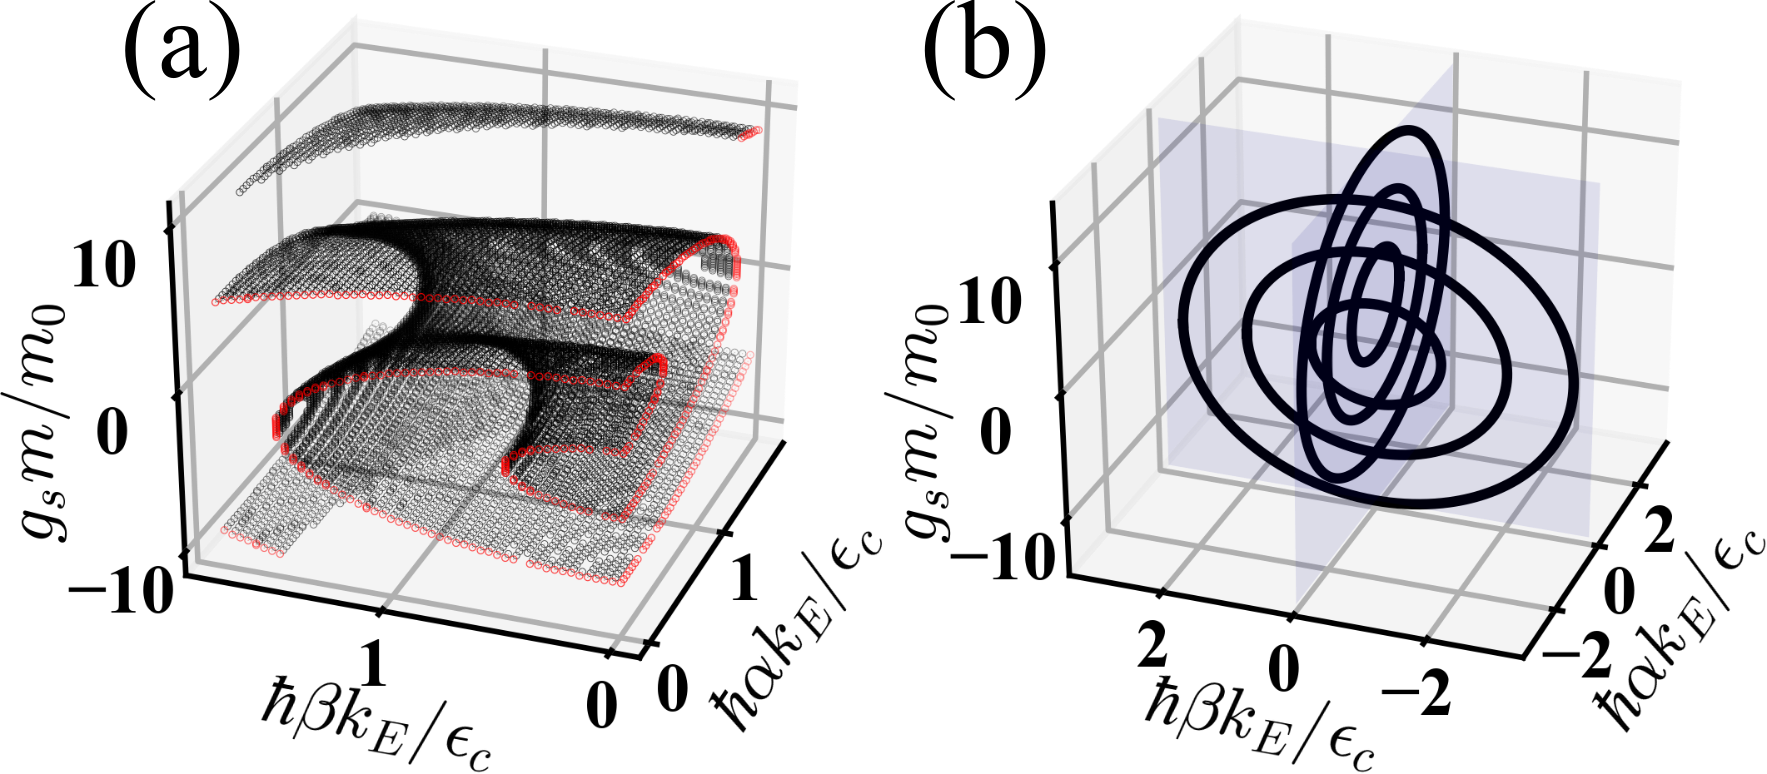
\includegraphics[width=1.0\columnwidth]{../figures/dgn.png}
	\centering
	\caption{Rashba-Dressalhaus模型的简并流形。 (a) $\A{=}I$的简并流形是一个道路连通的超曲面。 $\alpha=0$ 或者 $\beta=0$面上的点画成了红色。 (b) 阐释了$\A=-I$的简并流形,它处在$\alpha{=}0$和$\beta{=}0$面内(蓝色的半透明面)。这两个$\mathfrak{c}_{\infty}$对称的面都包含着无穷多的共心的圆。这两个面的圆相交在一起,因此整个流形是道路连通的 \label{fig:dgn}}
\end{figure}

\subsubsection{具有离散旋转对称性的Rashba-Dresselhaus二维电子气}\label{sec:disrot}

Rashba模型是一个过分的近似,连续旋转对称性不是任何晶体的对称性,连续旋转对称的$\bk{\cdot}\bp$模型仅仅是布洛赫哈密顿量的近似。那么如果连续旋转对称性微扰地降为离散的旋转对称性,上述的朗道能级的准简并会怎么变化呢?对于任意的整数$N{\geq}2$,我们发现$N$中的$N{-}1$个朗道能级准简并是稳定的,这一点的证明在附录\ref{app:codimension}。在这里,我们用一个$N{=}2$的模型来阐释上面的发现。我们要在Rashba模型中加入Dresselhaus自旋轨道耦合(耦合常数为$\beta$):
\begin{equation}
H_{RD}(\bk)=\frac{{\hbar^2}k^2}{2m}+\hbar\alpha(k_{x}\sigma_{y}-k_{y}\sigma_{x})+\hbar\beta(k_{x}\sigma_{x}-k_{y}\sigma_{y}).\label{hamRD}
\end{equation}
对于Rashba-Dresselhaus二维电子气,$\A$对$\alpha,~\beta,~l,~E,~m$参数的依赖并不是独立的,事实上,$\A$仅仅和下面三个参数有关
\e{\left( \f{\hbar\alpha k_{\sma{E}}}{\var_c},\f{\hbar\beta k_{\sma{E}}}{\var_c},g_{s\perp}\f{m}{m_0} \right){\in} \mathbb{R}^3. \la{parameter2}}
正如我们在\s{sec:ctsrot}所述,$\A(\hbar\alpha k_{\sma{E}}/\var_c,\hbar\beta k_{\sma{E}}/\var_c,g_{s\perp}m/m_0){=}{\pm} I$在$\beta{=}0$的平面上是一系列的共心圆。离开这个平面,我们发现$\A{=}I$在$\beta{=}0$平面附近仍然有解,也就是说,$\A{=}I$在$\mathbb{R}^3$中定义了一个超曲面,图\fig{fig:dgn}(a)画出了这个超曲面。另外一方面,$\A{=}{-}I$一般而言在$\beta{=}0$的附近并没有解,因此对应于$\A{=}{-}I$的圆仍然是孤立的,这一点可以从\fig{fig:dgn}(b)中看出来来。综上所述,我们发现每两个中的一个朗道能级准简并(也就是$j$为奇数的那个)在对称性降低下会消失

可以证明,$\A{=}I$的余维数为1的超曲面是来自$\mathfrak{c}_2$对称性。我们首先选取$\bk$无关的基(在这组基中泡利矩阵对应着自旋),写出对应的有效哈密顿量$\calh$ 
\e{\calh=\hbar\alpha (k_{x}\sigma_{y}{-}k_{y}\sigma_{x})+\hbar\beta (k_{x}\sigma_{x}{-}k_{y}\sigma_{y})-\f{g_{s\perp}}{2}\mu_{B}B\sigma_z,}
二重旋转对称性
\e{\calh(\bk)=\sigma_z\calh(-\bk)\sigma_z, \;\: \bk(t)=-\bk\big(t+\f{T_c}{2}\big)\in \frako_0,}
提示我们$[T_c/2,0]$时间段内的传播子和$[T_c,T_c/2]$时间段内的传播子是对称性联系起来的:
\e{\A=\A_{T_c\leftarrow T_c/2}\A_{T_c/2\leftarrow 0}=\sigma_z{\A}_{T_c/2\leftarrow 0}\sigma_z {\A}_{T_c/2\leftarrow 0}.\label{eq:sigmazconstraint}}
注意$\calh$的迹是零,所以${\A}_{\sma{T_c/2\leftarrow 0}}$的行列式是1。我们采用$\text{SU}(2)$矩阵的标准参数形式【参见式\ref{s3},其中 ${\cal \bar{A}}$替换为${\A}_{\sma{T_c/2\leftarrow 0}}$】,我们从\q{eq:sigmazconstraint}得到
\e{
	{\A}={\cal \bar{A}}(r_1,r_2,r_3)=\matrixtwo{1{-}2r_2(r_2{-}ir_1)}{2ir_2(r_3{+}ir_4)}{{-}2ir_2(r_3{-}ir_4)}{1{-}2r_2(r_2{+}ir_1)} \label{proprashba}
}
这里$\sum_{j=1}^4r_j^2{=}1$。\q{proprashba}就是二重旋转对称的传播子在对称坐标下的参数化表示。我们很容易发现$r_2{=}0$是$\A{=}I$的充分必要条件,对应的简并流形则是一个道路连通的超曲面,这个超曲面将$\br{=}(r_1,r_2,r_3)$空间分成了两份。在附录\ref{app:codimension}中,我们将这个结论扩展到了任意的$N{\geq}2$的情况:$\mathfrak{c}_N$对称的$\A$将对称坐标划分为$N$个道路连通的部分。\fig{fig:dgn}(a)展示了$\A=I$的在\q{parameter2}空间中的简并流形。

另外一方面,$\A{=}{-}I$当且仅当$\br{=}(0,{\pm} 1,0)$。这两个点映射到\q{parameter2}成为了$\alpha{=}0$和$\beta{=}0$的平面上的两条线【参见\fig{fig:dgn}(b)】:这个余维数的不同来自于这两个面满足$\mathfrak{c}_{\infty}$对称性【参见\s{sec:ctsrot}】,这一点在分析\q{proprashba}的$\mathfrak{c}_2$对称性的时候没有考虑在内。

\subsection{旋转对称磁隧穿}\label{sec:rotsymmbreakdown}

\begin{figure}
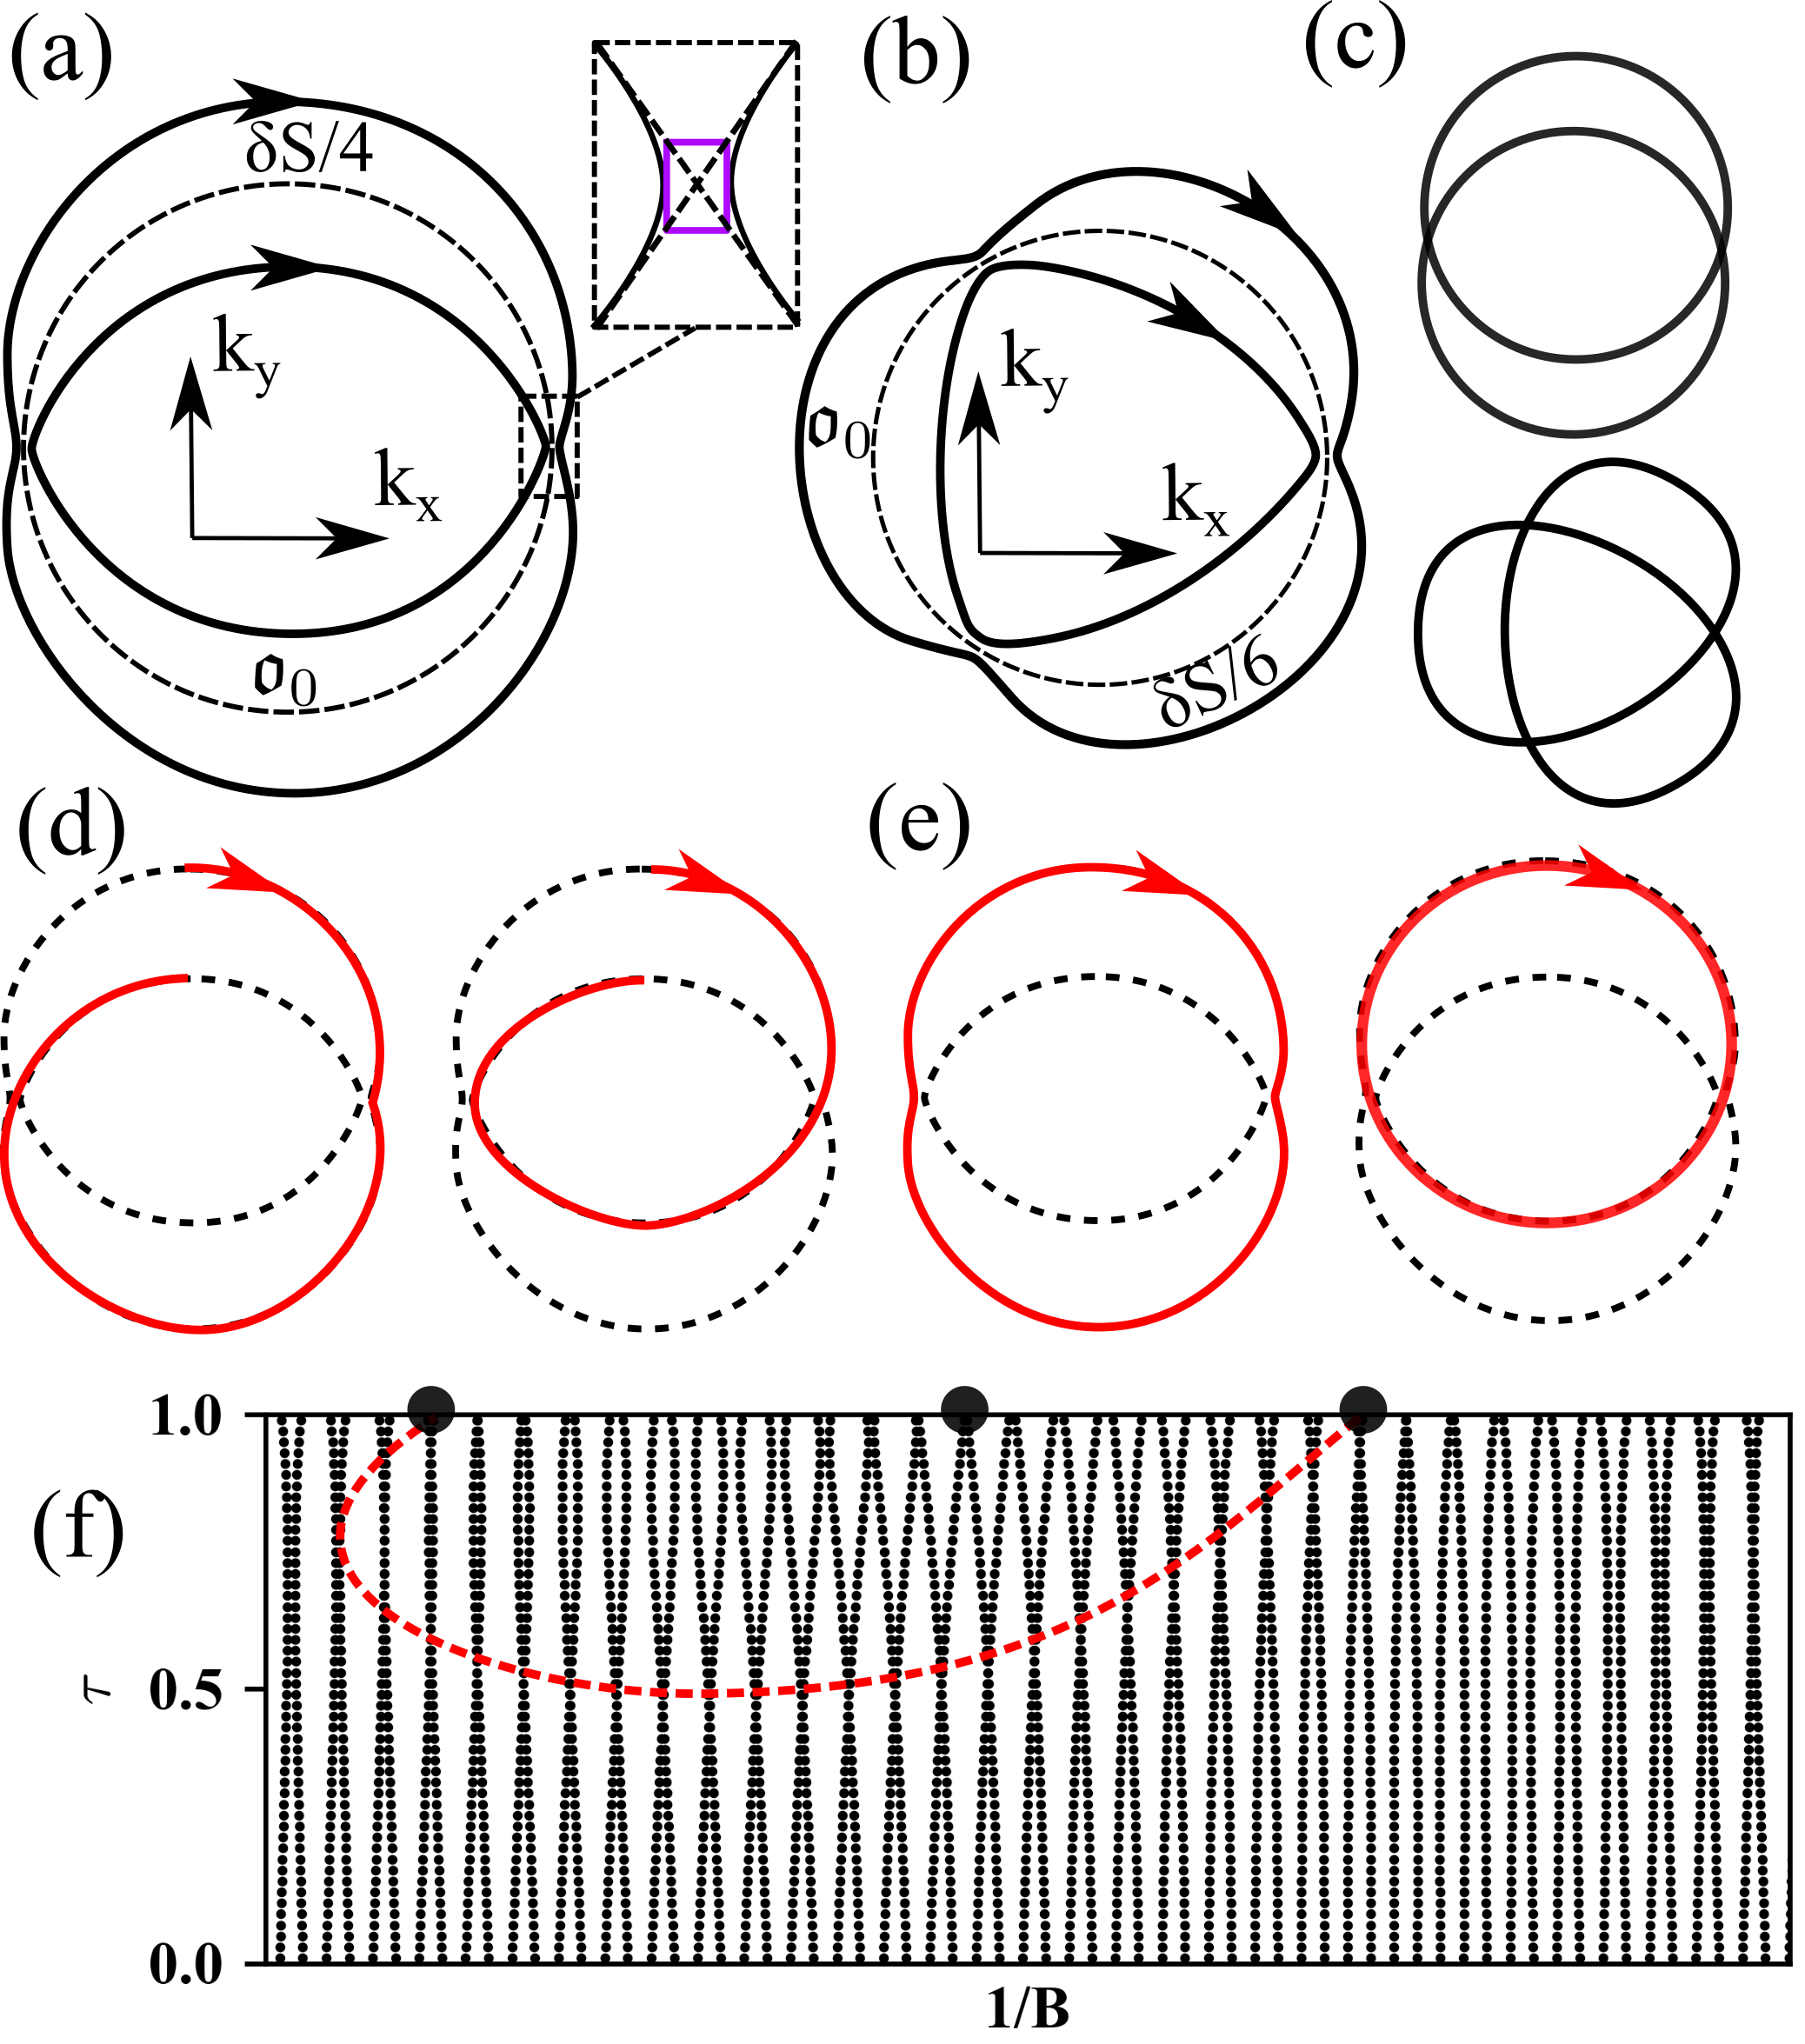
\includegraphics[width=0.8\textwidth]{../figures/Cn-breakdown.png}
\centering
\caption{(a-b) $\mathfrak{c}_2$对称【(a)】和$\mathfrak{c}_3$对称【(b)】的磁隧穿的磁振子轨道。(a)图的右上方展示了磁隧穿点附近的放大图,其中紫色的长方形的面积是$S_{\sma{\square}}$。 (c) $\mathfrak{c}_2$对称(上)和$\mathfrak{c}_3$对称(下)磁隧穿的Klein透射极限下的磁振子轨道。(d) 经过一次隧穿,改变了能带带标的费曼路径。(e) 经过零次或者两次隧穿,最终能带带标没有改变的费曼路径。(f) $\mathfrak{c}_3$对称的磁隧穿的朗道能级在能量固定的情况下相对$\tau$的色散图。在图中的$1/B$的区间,在$\tau=1$的时候有三个朗道能级简并点。当$\tau\ne 1$的时候,只有其中两个是稳定的,这两个朗道能级简并点在$\tau=0.5$的时候融合在了一起。\label{fig:Cn-breakdown}}
\end{figure}

对于近简并的能带,在绝热近似极限下,我们已经知道【参见\s{sec:introducecodimension}】$\cala{=}{\pm} I$的余维数为1。这里,我们要研究如果绝热近似被Landau-Zener隧穿破坏,但是仍然保持$N$重旋转对称性,余维数会有什么变化。由于第二类狄拉克点有一个确定的倾斜方向,它不可能作为旋转中心;因此,最简单的$\mathfrak{c}_N$对称并且含有第二类狄拉克点的模型需要由$N$个第二类狄拉克点。对于$N=2$,我们将要看到$\cala{=}I$(但是不是$\cala{=}-I$)的余维数是1,和前面\q{proprashba}的结果是一致的;这个结论可以从费曼路径的相干和相消的干涉现象理解。对于$N=3$,我们将要看到三个朗道能级准简并中的两个在微扰地加入Landau-Zener隧穿的时候是稳定的,但这两个在隧穿强度达到一定值的时候也会消失。


首先我们研究一个最简单的$\mathfrak{c}_2$对称的模型:
\e{H=\f{{\hbar^2}k^2}{2m_1}+ \bigg(\f{{\hbar^2}k^2}{2m_2}-\mu\bigg)\sigma_z +wk_y\sigma_x,\label{modelC2breakdown}}
其中$0{<}m_1{\ll}m_2$并且$\mu$是正的。$\mathfrak{c}_2$对称性体现在$\sigma_z H(\bk)\sigma_z{=}H({-}\bk)$上,并且将 
\e{\bar{k}_x = \pm\sqrt{2m_2\mu}/{\hbar},\;\bar{k}_y=0,\;\epsilon_{0}=\frac{m_2}{m_1}\mu.}
处的两个狄拉克点联系在一起。在这两个点附近,哈密顿量可以线性化为:
\e{H_{\pm} =\pm {\hbar}\sqrt{\f{2\mu}{m_2}}\bigg(\frac{m_2}{m_1}+\sz\bigg)\delta k_x+w\delta k_{y}\sx+\epsilon_0, \label{linearHam2}}
从这里我们可以看出如果$m_1{<}m_2$,那么两个狄拉克点都是第二类的。我们进一步假定$m_1{\ll}m_2$,这样近简并的条件($\delta S/S{\ll}1$)就能够得到满足。

在狄拉克点的能量($E{-}\epsilon_0 {\ll} wm_2(2\epsilon_0/m_1)^{\sma{1/2}}$)附近,磁振子轨道是两个共心的轨道,这两个轨道在两个狄拉克点处接近相交,图\ref{fig:Cn-breakdown}(a)中展示了这一点。在磁场足够小的情况下,带间的隧穿仅仅在第二类狄拉克点附近发生,其概率为
\e{\rho^2=e^{-2\pi\bar{\mu}}, \; \bar{\mu}=\f{\big(Z_{\perp}^2+(m_1/m_2)^2(E-\epsilon_0)^2\big)l^2}{2w\sqrt{2E/m_1}}. \label{landauzenerc2}}
另一中表达方式是$\bar{\mu}{=}S_{\sma{\square}}l^2/8$,其中$S_{\sma{\square}}$是两个双曲渐近线之间包围的正方形的面积【参见图\ref{fig:Cn-breakdown}(a)】。除了这两个狄拉克点,电子将会经历绝热(也就是保持能带不变的)演化。由于$\mathfrak{c}_2$对称性,整个磁振子轨道的传播子仅仅是半个磁振子轨道传播子的的平方:
\e{\A=\left(\matrixtwo{\tau e^{i\bar{\varphi}}}{-\rho}{\rho}{\tau e^{-i\bar{\varphi}}}{\diagmatrix{e^{i\tilde{\lambda}_-}}{e^{i\tilde{\lambda}_+}}} \right)^2. \label{propC2breakdown}}
半个磁振子轨道的传播子可以从\qq{scattmat}{propinplanezeeman}得到,其中$\bar{\mu}$由\q{landauzenerc2}给出,而$\tilde{\lambda}_{\pm}{=}{\pm}l^2\delta S/4$加上一个与磁场无关的相位修正。

$\cala$简并的充要条件是 
\begin{align}
\Delta:= \tilde{\lambda}_-{-}\tilde{\lambda}_{+}{+}2\bar{\varphi},\;\;
\tau\cos\f{\Delta}{2}= \begin{cases} 0, & {\A}=+I \\
                 \pm 1, & \A =-I\end{cases}.\label{c2breakdowndgncondition}
\end{align}
$\tau{=}1$和$\bar{\varphi}{=}0$的极限能够给出绝热演化的极限,此时\q{c2breakdowndgncondition}成立的条件就是$l^2$等于$2\pi/\delta S$加上一些和磁场无关的相位。

当绝热演化被破坏的时候,我们从\q{c2breakdowndgncondition}式中可以推断出$\A{=}I$仍然可以通过调节$B$得到,但是由于$\tau{<}1$,$\A{=}{-}I$不可能得到满足;这一点和\q{proprashba}的余维度分析是一致的。$\A{=}I$和$\rho{>}0$的条件可以理解为两个不同的隧穿一次的费曼路径的相消干涉【参见图 \ref{fig:Cn-breakdown}(d)】;与此同时,隧穿零次和隧穿两次的费曼路径则发生相干干涉【参见\ref{fig:Cn-breakdown}(e)】,因此朗道能级是准简并的。这样一个准简并在$\Delta$变化$2\pi$的时候重复发生,因此朗道能级准简并相对$l^2$的周期是$4\pi/\delta S$。这个周期并不会因为$\Delta$中$2\bar{\phi}$的存在而发生显著变化,因为$\bar{\phi}$只有$l^2$大致变化达到$2\pi/S_{\sma{\square}}$的时候才会发生显著变化,而$2\pi/S_{\sma{\square}}$要远大于$4\pi/\delta S$。综上所述,在引入磁隧穿之后,一半的朗道能级准简并消失,而另一半则保持稳定。如果$(\tau{=}0)$等于0【参见图\ref{fig:Cn-breakdown}(c)的上半部分】,那么这两个由$\mathfrak{c}_2$联系在一起,发生Klein隧穿的轨道是相同的,因此其朗道能级是简并的。


在文献\onlinecite{yakovenko_angular_2006}和文献\onlinecite{pershoguba_effects_2015}中,一个和本节模型完全不同的$\mathfrak{c}_2$的磁隧穿模型被提出,用以描述倾斜磁场中的双层金属。如果双层金属中的两层之间没有耦合,那每一层都有独立的磁振子轨道;从这个角度来看,层的自由度可以看成自旋1/2的自由度。如果两层之间有耦合,那么朗道能级仅仅在磁场方向取为特定的“魔角”的时候才会发生简并;这一点在文献\onlinecite{gusev_interlayer_2008}中得到了实验验证。不过在这些工作中,人们并没有认识到$\mathfrak{c}_2$对称性的作用。 


我们本节最后一个示例是$\mathfrak{c}_3$对称的第二类狄拉克点模型,这个模型画在图\ref{fig:Cn-breakdown}(b)中。在绝热近似满足的时候($\tau{\approx}1$),朗道能级准简并是周期性发生的;但是,在Klein-tunneling透射的极限,整个磁振子轨道是一个三叶草形的轨道【参见图\ref{fig:Cn-breakdown}(c)的下半部分】,因此所有的朗道能级都是非简并的,其间隔由这个三叶草轨道的有效质量决定。以上的特性对于任意奇数$N$的$\mathfrak{c}_N$对称的第二类狄拉克点模型都成立。

为了解决如上的矛盾,我们写出$\A$,其形式和\q{propC2breakdown}相似,仅仅是$(\cdot)^2$改为
$(\cdot)^3$,$\tilde{\lambda}_\pm{=}{\pm} l^2\delta S/4$改为$\pm l^2\delta S/6$(当然有可能由磁场无关的相位)。此时的准简并条件成为$\tau\cos[(\tilde{\lambda}_+{-}\tilde{\lambda}_-)/2{+}\bar{\varphi}]{=}{\pm} 1,{\pm} 1/2$。当磁隧穿发生的时候($1/2{<}\tau {<}1$),只有$\pm 1/2$是上式中可以取到的值。而在$\tau{=}1/2$的时候,所有的准简并全部两两湮灭。图\ref{fig:Cn-breakdown}(f)中展示了这一现象。


最后,我们提出,对于任意的正整数$N{\geq}2$,绝热极限下的每$N$个朗道能级准简并,在微扰地引入$\mathfrak{c}_N$对称的磁隧穿之后,$N{-}1$能够保持稳定,我们在附录\ref{app:codimension}中证明了这一点。

\subsection{余维数的对称性分类}\label{sec:tenfold}

\begin{table}
\begin{tabular}{|c|c|c|c|c|c|c|}
\hline 
轨道的变换 & $\boldsymbol{k}$的变换 & $u$ & $s$  & 标识 & $g$ & 余维数\tabularnewline
\hline 
\multirow{5}{*}{$|g\circ\mathfrak{o}_{0}|=|\mathfrak{o}_{0}|$} & \multirow{2}{*}{$\forall\boldsymbol{k}\in\mathfrak{o}_{0},g\circ\boldsymbol{k}=\boldsymbol{k}$} & \multirow{2}{*}{0} & \multirow{2}{*}{0} & \multirow{2}{*}{I-1} & $\breve{g}\propto I$  & 3\tabularnewline
\cline{6-7} 
 &  &  &  &  & $\breve{g}\not\propto I$  & 1\tabularnewline
\cline{2-7} 
 & \multirow{3}{*}{$\exists\boldsymbol{k}\in\mathfrak{o}_{0},g\circ\boldsymbol{k}\neq\boldsymbol{k}$} & 0 & 0 & II-1 & - & 1\tabularnewline
\cline{3-7} 
 &  & \multirow{2}{*}{1} & \multirow{2}{*}{1} & \multirow{2}{*}{II-2} & $g^{2}=1$  & 2\tabularnewline
\cline{6-7} 
 &  &  &  &  & $g^{2}=-1$  & 0\tabularnewline
\hline 
\multirow{2}{*}{$|g\circ\mathfrak{o}_{0}|\neq|\mathfrak{o}_{0}|$ } & \multirow{2}{*}{-} & 0 & 0 & III-1 & - & 3\tabularnewline
\cline{3-7} 
 &  & 1 & 1 & III-2 & - & 3\tabularnewline
\hline 
\end{tabular}
\centering
\caption{近简并能带的对称性限制的余维数,在这里,对称性被分为五类,名字写在第五列。
这个表格也适用于严格简并的能带,严格简并的能带中还由另外五类的对称性,另外五类在\tab{table:codimension-exactlydegen}中。第一列和第二列定义了对称性是怎么作用在磁振子轨道上的。下面的两列表征了$\bk{\rightarrow}g{\circ}\bk$【参见\q{gmapk}】保持($u{=}0$)或者没有保持($u{=}1$)磁振子轨道的方向,以及$g$含有($s{=}1$)或者不含有($s{=}0$)时间反演对称性。第六列对对称性的表示提出了一些额外的要求。$\breve{g}$是对角化过的近简并能带空间中$g$幺正表示。为了方便读者,我们在表格\ref{table:sewing-matrix}中列出了常见的对称性的表示矩阵。最后一列列出了对称性限制的余维数【参见第\ref{sec:introducecodimension}节】。\label{table:codimension-nearlydegen}}
\end{table}

\begin{table}
	\begin{tabular}{|c|c|c|c|c|c|c|}
	\hline 
	轨道的变换 & $\boldsymbol{k}$的变换  & $u$ & $s$  & 标识 & $g$  & 余维度\tabularnewline
	\hline 
	\multirow{5}{*}{$|g\circ\mathfrak{o}_{0}|=|\mathfrak{o}_{0}|$} & \multirow{2}{*}{$\forall\boldsymbol{k}\in\mathfrak{o}_{0},g\circ\boldsymbol{k}=\boldsymbol{k}$} & \multirow{2}{*}{0} & \multirow{2}{*}{1} & \multirow{2}{*}{I-2} & $g^{2}=1$  & 1\tabularnewline
	\cline{6-7} 
	 &  &  &  &  & $g^{2}=-1$  & 3\tabularnewline
	\cline{2-7} 
	 & \multirow{3}{*}{$\exists\boldsymbol{k}\in\mathfrak{o}_{0},g\circ\boldsymbol{k}\neq\boldsymbol{k}$} & 0 & 1 & II-3 & - & 1\tabularnewline
	\cline{3-7} 
	 &  & \multirow{2}{*}{1} & \multirow{2}{*}{0} & \multirow{2}{*}{II-4} & $\breve{g}\propto\sigma_{z}$  & 2\tabularnewline
	\cline{6-7} 
	 &  &  &  &  & $\breve{g}\propto\sigma_{z}$  & 0\tabularnewline
	\hline 
	\multirow{2}{*}{$|g\circ\mathfrak{o}_{0}|\neq|\mathfrak{o}_{0}|$ } & \multirow{2}{*}{-} & 0 & 1 & III-3 & - & 3\tabularnewline
	\cline{3-7} 
	 &  & 1 & 0 & III-4 & - & 3\tabularnewline
	\hline 
	\end{tabular}
	\centering
	\caption{五类适用于严格简并能带的对称性限制的余维度;另外五类在\tab{table:codimension-nearlydegen}中。我们采用和\tab{table:codimension-nearlydegen}一样的符号。在II-4类中, $\breve g$指的是$g$不变的$\bk$ ($g\circ\bk=\bk$)处的表示矩阵。对于I-2, II-3的II-4严格简并的轨道,假设自旋轨道耦合可以连续地去除,并且不会影响轨道地简并度,那么$\A$地行列式为1\cite{topoferm}。\label{table:codimension-exactlydegen}}
\end{table}

我们在本节将要推广第\ref{sec:singleparameterrashba}节到第\ref{sec:rotsymmbreakdown}节的内容,将对称性对余维度的限制推广到十类对称性上\cite{topoferm}。这十类对称性对应的余维数为$0,1,2$或者$3$。下面,我们首先在\s{sec:reviewtenfold}简要回顾一下磁振子轨道的十重对称性分类。然后,我们要在\s{sec:codimquasideg}中研究其中五类,这五类和近简并的能带相关。和严格简并的能带相关的另外五类将要在\s{sec:codimexactdeg}中研究。

\subsubsection{磁振子轨道的十重分类}\label{sec:reviewtenfold}

任意一个和没有磁场,具有离散平移对称性的哈密顿量$\hat{H}$的对称性$g$在时间和空间里作用为
\begin{align}
&g: \vectwo{\br}{t} \rightarrow \matrixtwo{\check{g}}{0}{0}{ (-1)^{s(g)}}\vectwo{\br}{t}+\vectwo{\bdelta}{0}, \label{definesg}
\end{align}
其中$s(g){=}0$($1$)对应着$g$保持(不保持)时间的方向。$\check{g}$是$g$在实空间的矩阵表示,$g$在晶体动量上的作用为
\e{\bk \rightarrow g\circ\bk := (-1)^{s(g)}\check{g}\bk. \label{gmapk}}
对于给定的$\hat{H}$以及给定的磁场方向,电子跟随着磁振子轨道进行回旋运动,磁振子轨道垂直于磁场。给定一个$\bk$空间的磁振子轨道,我们只关注能够保持磁振子轨道所在的$\bk$空间平面不变的对称性。这些对称性或者保持磁振子轨道不变(记为$|g\circ\frako|{=}|\frako|$)或者将磁振子轨道映射到另外一个磁振子轨道($|g\circ\frako|{\ne}|\frako|$)。前一种情况还可以分为两类:(a)$g$将磁振子轨道上的每个$\bk$都映射到自己;(b)磁振子轨道上至少有一个$\bk$没有被$g$映射到自己。

最后,我们还需要区分【参见\q{gmapk}】保持磁振子轨道方向或【$u(g){=}0$】者不保持磁振子轨道方向【$u(g){=}1$】的对称性。比如旋转轴在沿着磁场方向的旋转就能够保持轨道的方向,而镜面反射则会改变磁振子的方向。上述的所有的对$g$的描述将对称性分为十类,这十重分类是文献\onlinecite{topoferm}首次提出的。这十类对应着表格\ref{table:codimension-nearlydegen}和表格\ref{table:codimension-exactlydegen}的十行。

\subsubsection{近简并轨道的对称性限制的余维数}\label{sec:codimquasideg}

在近简并轨道中,哈密顿量$\hat{H}{=}\hat{H}_0{+}\delta \hat{H}$是具有简并能带的零阶哈密顿量和破坏对称性的扰动哈密顿量的和。给定一个$\hat{H}_0$的零阶轨道$\frako_0$,我们现在关注$\hat{H}$的对称性中,能够将$\frako_0$变为自己或者另一个零阶轨道的那些对称性。


在\s{sec:reviewtenfold}所述的十重对称性分类中,只有五类是和近简并轨道相关的,这是因为我们的量子化条件中的$\lambda_a$是由$\A$决定的【参见\q{eq:prop}】,而$\A$则是由$\H{=}\delta\epsilon{+}B \mathcal{M}$【参见\q{eq:H1}】的演化子构成的。$\H$包含了$\frako_0$上的$\delta H$和塞曼作用项。由于$g$是$\delta \hat{H}$的对称性,$\delta\epsilon$在$g$的作用下是不变的。另一方面$\mathcal{M}$ 是平行于磁场方向的的赝矢量,在时间反演对称性\cite{sakurai1995modern}下会反号,因此在$g$的变换下是变为$(-1)^{u+s}\mathcal{M}$(加上一项和规范相关的项\cite{100p}),只有$u{+}s{=}0$或者$2$才能够保证$\H$在$g$下有一个相容的变换,这个条件就给出了表格\ref{table:codimension-nearlydegen}中的五类。

对于这五类,我们将其对应的余维度写在表格\ref{table:codimension-nearlydegen}的最后一列,这些结果的推导在附录\ref{app:codimension}里。我们在这里要强调余维数就是找到$\A$的简并点需要调整的参数的个数。我们在表格中列出的余维数在任何保持对应的对称性(并且保持磁振子轨道的拓扑形状)的扰动下都不会发生变化。
 
在这五类对称性中,只有第I-1, II-1和II-2的余维度可能小于3,因为只有这三类对称性能够将磁振子轨道映射到自己。这三类对称性将$\A$和它自己或者它自己的逆联系在一起,因此可以降低其简并流形的余维数。

I-1类包含了所有让磁振子轨道上的点$\bk$映射到自己的所有空间对称性。最简单的例子是镜面对称性$\mathfrak{m}_z$,其中$-z$是磁场的方向,并且磁振子轨道在$\mathfrak{m}_z$不变的平面内。要确定对称性限制的余维数,我们需要知道两条近简并的能带对应的是$g$的相同的表示还是不同的表示。如果是不同的表示,那么能级排斥就不会存在,此时余维度为1。

II-1类则对应着保持磁振子轨道方向不变的空间对称性,其中一个重要的例子就是旋转对称性,另一个例子是空间反演对称性,对于空间反演对称性,我们要求$\frako_0$在空间反演不变的面上:$k_z=0$或者$\pi$。正如我们在第\ref{sec:singleparameterrashba}节到第\ref{sec:rotsymmbreakdown}节描述的那样,此时的余维数是1。对于一个确定的II-1类中的$\frako_0$,不同的简并流形可能有着不同的余维数,此外我们列出的余维数是最小的余维数。比如说,我们发现二重旋转对称性将$\A{=}{+}I$的余维数限制为1,而$\A{=}{-}I$的余维数还是3【参见\fig{fig:dgn}和\q{proprashba}】,我们就在表格中II-1的最后一列填上3。


II-2反转了时间的方向,也反转了磁振子轨道的方向。此时,如果$g$的平方是$+1$,那么余维数是2,而如果$g$的平方是$-1$,那么余维数是0。一个前者的例子是时间反演和镜面反射的联合操作(镜面反射轴垂直于磁场方向);Rashba-Dresselhaus哈密顿量就有这样的对称性【参见\q{hamRD}】:
\e{g H_{RD}(k_x,k_y)g^{-1} = H(k_y,k_x),\;\; g = e^{i\sigma_z\pi/4}K,}
其中$K$是复共轭。这个对称性也可以解释图\ref{fig:dgn}(b)中的简并流形并不是点,而是线,这一点我们之前是用连续旋转对称性解释的。


一个$g^2{=}-1$的例子则是一个时间反演和滑移面的组合$T\mathfrak{r}_{x,\boldsymbol{c}/2}$;滑移面$\mathfrak{r}_{x,\boldsymbol{c}/2}$是一个镜面反射(轴垂直于磁场方向)和半个晶格矢的平移(平行于磁场方向)的组合。这种情况下布里渊区边界($k_z{=}\pi$平面)上的磁振子轨道对应的朗道能级就是简并的(其原因与Kramers类似),此时余维度为0。

最后,我们指出,在第\ref{sec:inplanezeeman}节中研究的倾斜磁场中的Rashba二维电子气,同样属于II-2类轨道,其对称性为
\begin{equation}
\sigma_z K H_{RZ}(k_x, k_y) K \sigma_z=H_{RZ}(k_x, -k_y).
\end{equation}
因此,简并流形在参数空间$(\alpha, B_\parallel, g_{s\perp})$表现为线。我们数值上确定了这些线是在 $B_\parallel=0$和$\alpha=0$平面内。这两个面内的朗道能级都是精确可解的。对于$B_\parallel=0$,$H_{RZ}$就退化为Rashba哈密顿量,其简并流形是一系列的共心圆【对应图\ref{fig:dgn}(b)中$\beta=0$的平面】。对于$\alpha=0$,简并流形则在
\begin{equation}
    \f{g_s}{4} \frac{ m}{ m_0}\text{sec}(\theta)=n,\;\;(n\in\mathbb{Z}),
\end{equation}
处,其中$\theta$是磁场的倾斜角:$\cos(\theta)=B_\perp/\sqrt{B_\perp^2+B_\parallel^2}$。


\subsubsection{严格简并的轨道的对称性限制的余维数}\label{sec:codimexactdeg}

我们的工作主要集中在近简并轨道的量子化条件里,此时没有磁场的哈密顿量写为$\hat{H}_0{+}\delta \hat{H}$。在这一小节,我们关注对称性更高的晶体,这些晶体的$\delta \hat{H}$被禁戒。$\hat{H}_0$有可能包含自旋轨道耦合也有可能不包含自旋轨道耦合,如果包含自旋轨道耦合,那么能带在每个$\bk$点的简并需要一些对称性来保护(比如$T\inv$时间空间反演对称性)。


给定了$\hat{H}_0$以及磁场的方向,不同自旋的电子遵循着严格相同的轨道(还是用$\frako_0$)标记。这样的轨道我们成为严格简并的磁振子轨道,而近简并的磁振子轨道在$\bk$空间则会劈开。尽管轨道是简并的,朗道能级一般而言由于塞曼相互作用$B\calm$是劈开的。对于严格简并的轨道,我们同样要研究,多少个实的参数可以调节到一个朗道能级的准简并。


我们的研究方式和近简并的轨道的研究方式是基本相同的:严格简并的轨道的量子化条件\cite{topoferm}和\qq{eq:rule}{berryconn}形式一致,只需要$\delta \var{=}\delta S{=}0$。$\A$的本征值简并同样对应着朗道能级准简并,\s{sec:relatedegeneracies}的分析在这里同样适用。

但是,严格简并轨道的对称性类可以更多一些,在\s{sec:codimquasideg}中,我们只关注让磁矩$\calm$不变(加上一个规范有关的常数\cite{100p})的对称性,这样$\calh{=}\delta \var{+}B\calm$中的两项才能够遵守相同的变换规则。但是由于在严格简并能带中$\delta\var{=}0$,因此我们也允许将$\calm$翻转的对称性。

很多翻转$\calm$的对称性也会导致余维数小于3,这一点对应着\tab{table:codimension-exactlydegen}中的五个对称性分类。比如说,II-2中的对称性同时翻转时间和$\calm$,并且将每个$\frako_0$上的$\bk$点映射到自己。如果$g$的平方是$-1$(比如$T\inv$对称性),那么余维数是3,如果$g$的平方是$+1$(比如$T\rot_{2z}$,也就是时间反演和二重旋转的组合操作),那么余维数是1。对于处在$\rot_{2z}$不变的平面内的严格简并的轨道$\frako$,$\A$和一个特殊正交矩阵是幺正相似的\cite{100p,alexandradinata_berry-phase_2016},因此唯一的一个可调参数就是旋转角,因此余维数是1。


最简单的保持$\calm$的对称性是I-1中的连续自旋旋转对称性。这个对称性是任何自旋轨道耦合可以忽略的固体都具有的对称性。由于不同自旋的电子朗道能级没有能级排斥,余维数显然是1【参见\tab{table:codimension-nearlydegen}中的I-1的本征值不同的那一行】。

所有的十类对称性的具体例子的研究将留到以后的研究工作中。最后,我们提一下对于严格简并的轨道,哪些实验参数是容易调的。由于$\delta\var$的缺失,$\cala$的本征值是和$B$的大小无关的【参见\q{eq:Rashba-lambda}并将其中的$\delta S$设为0】.但是由于塞曼效应一般而言是各向异性的,我们可以调节磁场的方向,我们同样可以通过调节隧穿谱的偏压来调节朗道能级的能级指标。

\begin{table}
\begin{tabular*}{\columnwidth}{c@{\extracolsep{\fill}}ccc}
\hlineB{2.0}
类别 & 对称性  & 简并的起源 & $\breve{g}\propto$ \\
\hline 
\multirow{2}{*}{I-1} & \multirow{2}{*}{$\mathfrak{r}_z$, $\mathfrak{r}_{z,\boldsymbol{a(b)}/2}$} & $T\mathfrak{i}$, spin $\text{SU}(2)$ & $\sigma_z$ \\
\cline{3-4}
 & & $T\mathfrak{c}_{2z,\boldsymbol{c}/2}$ & $I$ \\
\hline
\multirow{3}{*}{I-4} & $\mathfrak{r}_{x(y),\boldsymbol{c}/2}$ & $T\mathfrak{i}$, spin $\text{SU}(2)$, $T\mathfrak{c}_{2z,\boldsymbol{c}/2}$ & $\sigma_z$ \\
\cline{2-4}
& $\mathfrak{r}_{x(y)}$,$\mathfrak{r}_{x(y),\boldsymbol{b(a)}/2}$, & $T\mathfrak{i}$, spin $\text{SU}(2)$ & $\sigma_z$ \\
\cline{3-4}
& $\mathfrak{c}_{2x(y)}$, $\mathfrak{c}_{2x(y),\boldsymbol{b(a)}/2}$ & $T\mathfrak{c}_{2z,\boldsymbol{c}/2}$ & $I$\\
\hlineB{2.0}
\end{tabular*}
\caption{镜面(例如$\mathfrak{r}_x$), 旋转(例如$\mathfrak{c}_{2y}$),滑移面(比如$\mathfrak{r}_{x,\ba/2}$)和螺旋轴(比如$\mathfrak{c}_{2y,\ba/2}$)的表示矩阵。后两个非点式的对称性含有$x,~y,$或者$z$方向半个晶格格矢的平移(用$\boldsymbol{a,~b,~c}$标识)。我们的$-z$轴是磁场的方向。这个表格可用于严格简并的轨道,其中轨道的简并来自于时间和空间的反演$T\mathfrak{i}$,二重螺旋轴和时间反演的组合$T\mathfrak{c}_{2z,\boldsymbol{c}/2}$(适用于$k_z=\pi$平面的轨道)以及自旋$\text{SU}(2)$对称性(也就是自旋轨道耦合可以忽略)。\label{table:sewing-matrix}}
\end{table}

\section{近简并和严格简并轨道的量子振荡}\label{sec:qo}

在\s{sec:qtznrules}中我们给出了无论是近简并($0{<}\delta S{\ll}S$)还是严格简并($\delta S{=}0$)的轨道都适用的量子化条件【参见\qq{eq:rule}{berryconn}】。这一节,我们将要研究这个量子化条件对Shubnikov-de Haas(SdH)\cite{SdH}量子振荡和de Haas-van Alphen(dHvA)\cite{dHvA}量子振荡现象的影响。在\s{sec:quantosc_equidis}中,我们给出一个推广的Lifshitz-Kosevich公式\cite{lifshitz_kosevich,lifshitz_kosevich_jetp}。这个公式只需要输入我们的量子化条件就可以得到量子振荡的图案。将这个公式用在高温情况下,我们将要证明最低阶量子振荡只需要一个参数就可以调到相消的振荡,这个参数可以是磁场$B$本身。\s{sec:quantosc_quasideg}则关注在对称类I-1和II-1中【参见\tab{table:codimension-nearlydegen}】近简并轨道的低温SdH振荡,我们将要预言在固定粒子数密度的假设下,在调节$B$的时候,一个周期加倍和周期不加倍之间连续变化的量子振荡。


\subsection{单参数调节最低阶振荡的相消现象}\label{sec:quantosc_equidis}


Lifshitz-Kosevich公式\cite{lifshitz_kosevich,lifshitz_kosevich_jetp}给出了量子振荡的所有分量。这个公式首先在I-1类中被导出\cite{rothmag},后来被推广到了任意的对称类中\cite{topoferm}。一个非常简单的推广就能让文献\onlinecite{topoferm}中的公式适用于近简并的轨道。比如说,二维的磁矩的振荡可以用下面的式子表示
\begin{equation}
\delta M=-\frac{1}{2\pi}\frac{k_BT}{BS^{-1}}\sum_{a=1}^2\sum_{r=1}^{\infty}e^{-\f{r\pi}{\omega_c\tau_{\sma{D}}}} \frac{\text{sin}[r(l^2S{+}\lambda_a{+}\gamma)]}{\text{sinh}(2\pi^2rk_BT/\var_c)},\label{eq:LK}
\end{equation}
其中sine函数内的量来自于我们的的量子化条件【参见\qq{eq:rule}{berryconn}】,$T$是温度,$\tau_{\sma{D}}$是Dingle散射寿命\cite{Dingle_collisions}。右手边所有的量都是在化学势处计算的。

在高温的时候($kT{\gg}\var_c$)或者散射很强的时候($\omega_c\tau_{\sma{D}}{\ll}1$),$\delta M$中最重要的贡献来自于最低阶的振荡($r{=}1$)。如果$\delta \lambda{=}|\lambda_1{-}\lambda_2|{\equiv}0$,那么这个求和是相干的,如果$\delta \lambda{\equiv}\pi$,那么这个求和是相消的。这里$\equiv$指的是模$2\pi$的相等。如果最低阶震荡相消,那么只有偶数阶振荡才会显示出来。

我们已经在\s{sec:llquasideg}中展示了调节到$\delta \lambda{\equiv}0$所需要的参数的个数;这个数目可以看成一个对称性相关的,度量朗道能级之间的排斥程度的量【参考\tab{table:codimension-nearlydegen}和\tab{table:codimension-exactlydegen}】。正如图\ref{fig:qo}(b)所示,$\delta \lambda{\equiv}\pi$是朗道能级之间间隔几乎相等的条件,其值为${\approx}\var_c/2$。由于不需要能级相交,我们认为(任意的对称类中)$\delta \lambda{\equiv}\pi$只需要最多一个参数就可以调节到。要证明这一点,我们接着来看$\text{SU}(2)$矩阵${\cal \bar{A}}$的标准参数化【参见\q{s3}】。$\delta \lambda{\equiv}\pi$的充要条件是${\cal \bar{A}}(r_1,r_2,r_3)$的本征值是$+i$和$-i$;这等价于$r_1{=}0$,只需要一个参数。

对于严格简并的轨道,这个相消干涉的单参数调节可以通过化学势【这一点在文献\onlinecite{topoferm}中做出了说明】或者磁场的取向来做到。此时,在我们目前的解的精确度下, $\lambda_a$和磁场的强度时没有关系的\cite{rothmag,fuchs_landau_2018,gao_zero-field_2017,fischbeck_review},这一点我们在\s{sec:codimexactdeg}提到过。

对于近简并的轨道,$\lambda_a$可以展开为$B$的一个洛朗级数,最高阶项为$1/B$【参见\q{lambdasmallB}】,因此$B$可以用来调节得到相消干涉。由于$\lambda_a$相对于$l^2S$是缓慢变化的,我们应该会看到一个最低阶振荡的拍的现象。在绝热近似成立的情况下,这个拍的节点是随着$l^2$周期性出现的【参见\s{sec:introducecodimension}】,周期是$2\pi/\delta S$,但是在非绝热演化的情况,由于能带之间的混合,这个周期性一般是丢失了【参见\q{lambdasmallB}】。

这样的拍的现象已经在半导体异质结\cite{das_evidence_1989,hu_zero-field_1999,wilde_inversion-asymmetry-induced_2009}或者非中心反演的晶体\cite{terashima_fermi_2008,onuki_chiral-structure-driven_2014,maurya_splitting_2018}中发现了。在绝大部分实验中,拍被用来推测自旋轨道耦合的强度\cite{das_evidence_1989,onuki_chiral-structure-driven_2014,maurya_splitting_2018},其中一部分实验\cite{das_evidence_1989}注意到了拍的非周期性现象,并且归因于$B$依赖的轨道劈裂,对应着不同的(对应于$1/B$的)频率$f_1$和$f_2$。在我们的语言中,$|f_1-f_2|=B\delta\lambda/2\pi$,其中最高阶项$\delta \lambda(E,B)$正比于$1/B$。

我们的贡献是一个定量的计算$\delta\lambda$和$B$的计算理论,我们将次高阶项$({\sim}B^0)$归因于广义的塞曼效应,更高阶项归因于自旋轨道耦合和塞曼效应的竞争【参见\q{eq:Rashba-lambda}】。举个例子来说,我们可以得到Rashba系统或者Rashba-Dresselhaus二维电子气中拍的节点之间的($1/B$轴上的)距离。


\begin{figure}
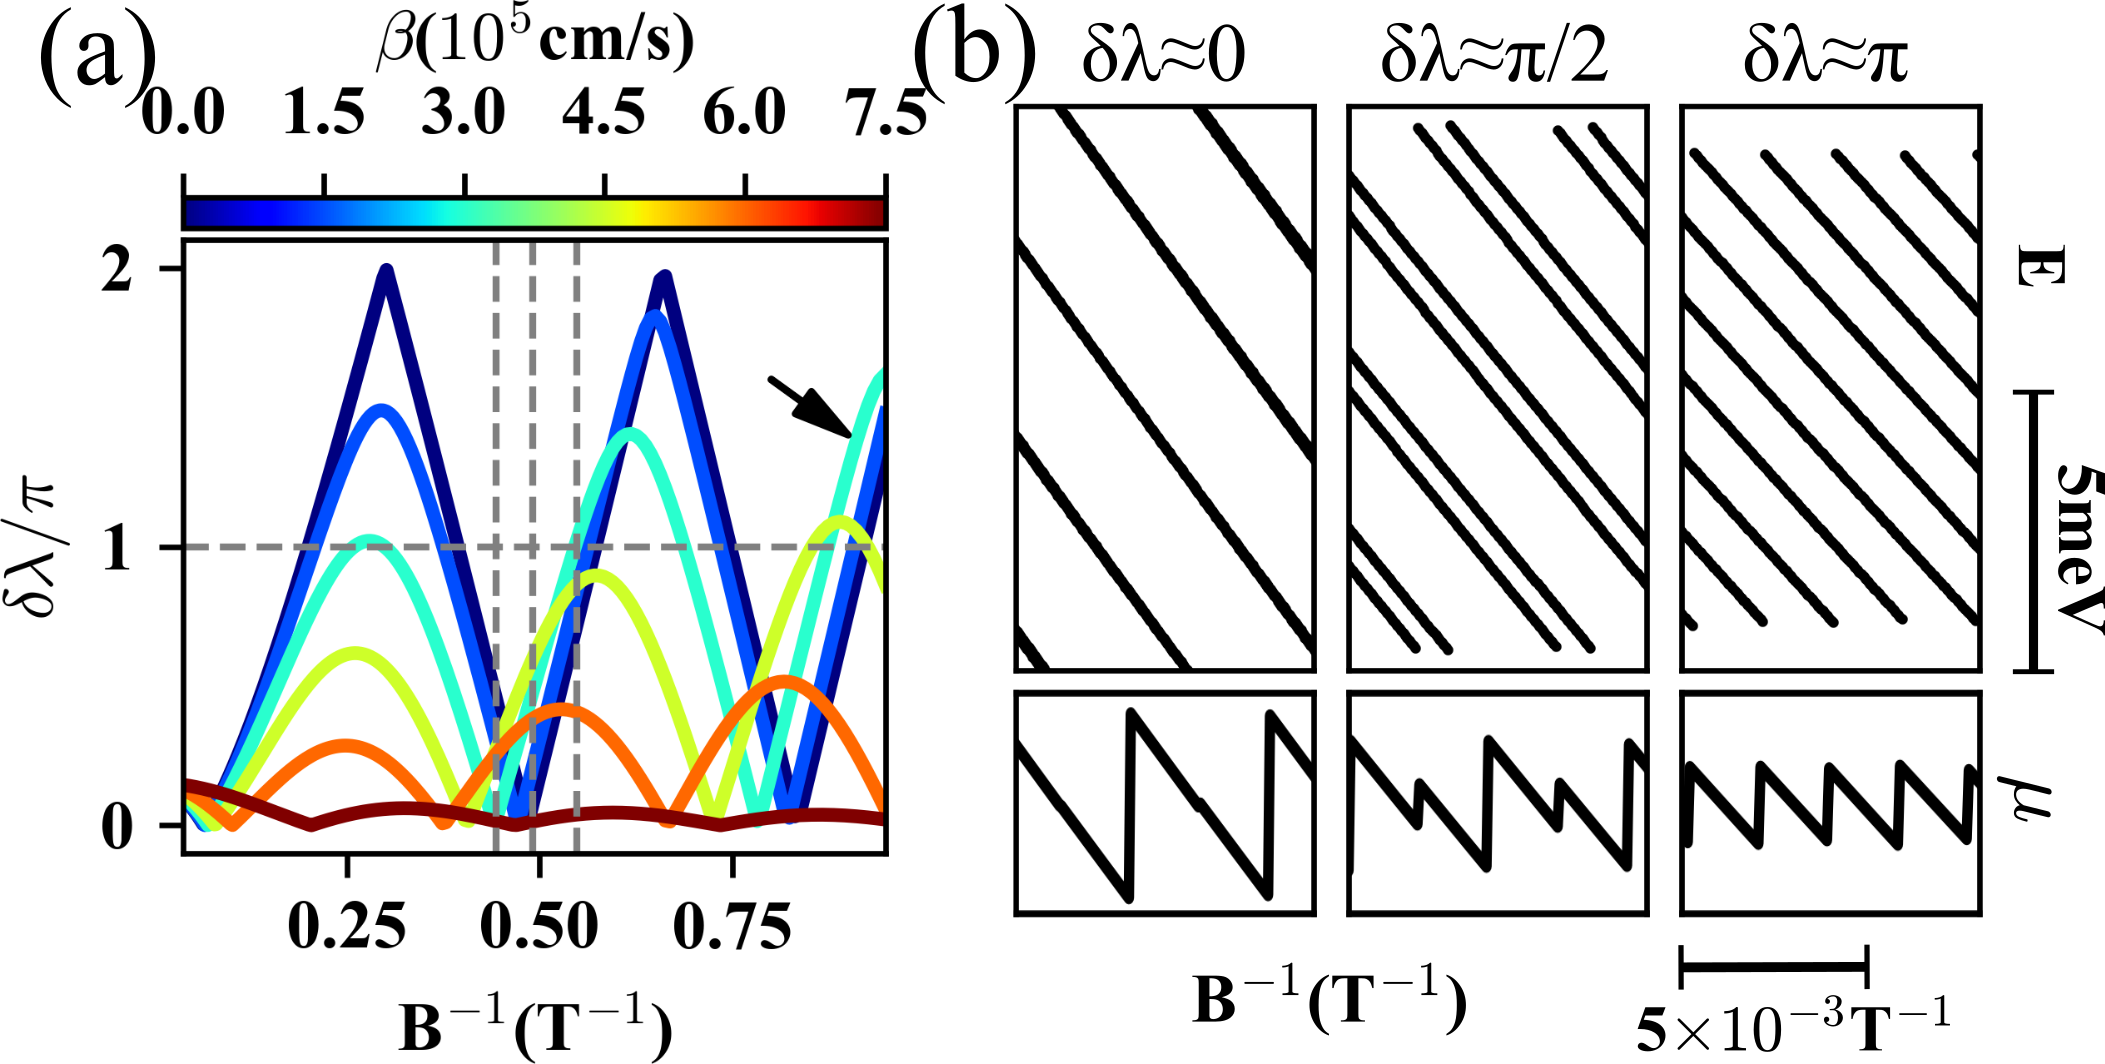
\includegraphics[width=1.0\textwidth]{qo.png}
\caption{Rashba-Dresselhaus二维电子气的量子振荡。 (a) $\delta\lambda$在不同的$\beta$值下随着$1/B$的变化。横向的虚线表示的是$\delta\lambda=\pi$。在$\beta=3.0\times 10^{5}$cm/s的情况下,我们在(b)的上半部分画出了三个$B$值【对应着(a)中的三条虚线】处的朗道能级。此时$\delta \lambda$在(a)中画成了蓝绿色;三个选出来的$B$分别对应于$\delta\lambda{=}0$, $\delta\lambda{=}\pi/2$以及$\delta\lambda{=}\pi$。(b)的下半部分画出了(固定粒子数密度的情况下)锯齿形的化学势的振荡,它们和(b)的上办部分是对应的。(b)中的其他参数为$m{=}0.076m_0$, $\alpha{=}7.5\times10^{5}$cm/s和$E=0.4$eV.
\label{fig:qo}}
\end{figure}

\subsection{对称类I-1和II-1中近简并轨道的Shubnikov-de Haas效应}\label{sec:quantosc_quasideg}

让我们现在关注单参数就能调节到$\delta \lambda{\equiv}0$的近简并轨道。这样的轨道属于I-1和II-1对称类,对于I-1,我们对对称性的表示矩阵有进一步的要求,具体参见\s{sec:codimquasideg}和\tab{table:codimension-nearlydegen}。

我们提出,要观测到这样的单参数可调性,我们可以采用固定粒子数密度$n_e$,低温($k_BT{\ll}\var_c$),无序很少($\omega_c\tau_{\sma{D}}{\gg}1$)的Shubnikov-de Haas效应。在这个参数范围内,我们知道纵向电导在一些离散的磁场大小的时候(记为$B_{\nu}$)会达到最小值,此时朗道能级被整个占据\cite{vinter_resolution_1980};量子振荡的周期是由总的电子密度$n_e$决定的:$1/B_j{-}1/B_{j+1}{=}e/n_eh$。在$B$增加穿过$B_j$的时候,一个朗道能级上的电子全部消失,导致化学势($\mu$)的周期性的突然下降,这一点体现在\fig{fig:qo}(b)中。每当$\delta\lambda{\equiv}\pi$,朗道能级之间的间距是完全相同的,所以相邻的化学势(也体现在电导上)的下降时基本相同的;每当$\delta\lambda{\equiv}0$,每隔一个的化学势的下降就会消失\cite{bychkov_oscillatory_1984}。$0{\leq}\delta\lambda{\leq}{\pi}$ 因此会体现为一个周期加倍和不加倍的振荡之间的连续变化,这一点展示在\fig{fig:qo}(b)中

我们的贡献是完备地找到了两个对称性类(I-1 and II-1),在这两个类中会发生这样一个周期加倍和不加倍的振荡的连续变化。特别地,我们提出这样的现象会发生在Rashba-Dresselhaus二维电子气中【参见\q{hamRD}】。对于这个模型,图\ref{fig:qo}(a)展示了在不同$\beta$参数下$\delta \lambda$对$1/B$的关系。正如我们在\s{sec:disrot}余维数的分析,一半的简并点会在加入不为零的$\beta$的时候消失。

\section{总结和讨论}\label{sec:discussion}

我们将准经典理论中的Landau量子化推广到了近简并的磁振子轨道,也就是$\bk$空间劈裂的面积差($\delta S$)远小于平均面积的情况。对于两条近简并能带的情况,我们的量子化条件总结在\qq{eq:rule}{berryconn}里。这个量子化条件可以应用于自旋轨道耦合导致的或者是对称性破坏导致的自旋劈开的轨道。前者的例子之一就是我们对Rashba-Dresselhaus二维电子气在任意方向磁场中的案例分析。

我们量子化条件【参见\q{eq:rule}】中的次低阶的的相位修正($\lambda_1,\lambda_2$)包含了轨道劈裂导致的动力学修正以及推广的两带的塞曼作用。如果在某一个具体的能量$E$和磁场$B$的时候,$\lambda_1{=}\lambda_2$ mod $2\pi$,那么在这个能量和磁场附近,会由成对的接近简并的朗道能级。这样的接近简并的朗道能级被称为准简并,朗道能级准简并的可以在示意图\ref{fig:LL}中看出来。


对于五个近简并轨道的对称类,我们确定了需要找到一个朗道能级准简并需要调节的实参数的数目;这个数目可以看成对称性相关的朗道能级相互排斥的量化指标。我们将这个数目成为对称性限制的余维数。不同的对称类具有不同的余维数,其取值可能是0,1,2,3,我们的结果总结在表\ref{table:codimension-nearlydegen}和表\ref{table:codimension-exactlydegen}里。

如果余维数是1,那么对于近简并轨道,我们可以仅仅通过调节$B$的大小来找到朗道能级准简并。我们在\s{sec:quantosc_quasideg}中讨论了这一点在Shubnikov-de Haas振荡中的体现。如果余维数是2,那么我们需要再多调节一个参数才能找到朗道能级准简并,这个参数可以是磁场的取向\cite{yakovenko_angular_2006},或者朗道能级的指标(通过调节隧穿谱的偏压)\cite{Sangjun_Cd3As2,Ilija_SnTe,kushwaha_Dirac}。我们在本章主要讨论了二维系统中的朗道能级,但是在三维系统中,平行于磁场方向的晶格波矢也是一个可调参数。


我们在这里要特别提出表格\ref{table:codimension-nearlydegen}中的一项(II-1):对于具有旋转对称性或者空间反演对称性的哈密顿量和磁振子轨道,余维数是1,这两个对称性在实际材料中经常出现。从几何的角度来看,这个对称类中的朗道能级准简并在可调参数空间中是一个超曲面。从拓扑的角度来看,这个超曲面是参数空间的畴界,将参数空间分成了多个连通的部分,如果旋转对称性是$N$重的,那么连通的部分就有$N$个。这个$N$重旋转对称性拓扑上的区别意味着如果旋转的重数降低,那么其中一部分的朗道能级准简并将会消失,另一部分则保持稳定。这一点在\s{sec:singleparameterrashba}中针对Rashba-Dresselhaus二维电子气得到了充分的研究。另外,向列性的相变经常伴随着旋转对称性重数的减小\cite{fradkin_nematic_2010};因此,我们有可能通过朗道能级准简并的稳定性来判断向列性的相变是否会发生。

作为近简并的特例,我们的量子化条件【\qq{eq:rule}{berryconn}】可以用在严格简并的轨道里。严格简并指的是磁振子轨道在每个点$\bk$点严格重合。严格简并的磁振子轨道的对称性特征被分为十类,比近简并多五类。对于每一类,我们也得到了其对称性约束的余维数,结果展示在表格\ref{table:codimension-nearlydegen}至\ref{table:codimension-exactlydegen}。严格简并和近简并的轨道还有一个区别:磁场的强度一般而言不能够调节严格简并轨道的$\lambda_1,\lambda_2$,但是我们仍然可以通过磁场的方向和朗道能级的指标来调节$\lambda_1,\lambda_2$。


我们的余维数分析不仅仅局限于朗道能级的排斥。如果我们仅仅考虑\q{eq:H1}中的贝里联络,那么\q{eq:prop}则会退化为Wilson圈\cite{wilczek_appearance_1984}。因此,Wilson圈也能够被分为十类,同样遵循着\tab{table:codimension-nearlydegen}至\tab{table:codimension-exactlydegen}中的余维数的分析。因此,我们的工作也能够解释Wilson圈的本征值里稳定的交叉,这些交叉在拓扑能带论里得到了广泛的应用。比如说,这样的交叉的存在曾经被用来分析旋转对称性保护的三维的狄拉克点\footnote{文献\onlinecite{gresch_z2pack:_2017}数值上观测到了相应的现象,其解释可以在文献\onlinecite{100p}和文献\onlinecite{li_topological_2017}中找到。},以及存在旋转对称性的脆弱拓扑相\cite{bouhon_wilson_2018,bradlyn_disconnected_2018}。


对称性不仅仅限制了$\lambda_1$和$\lambda_2$之间的能级排斥,在一些特定的对称类里,对称性也会限制他们的和。在我们之前的工作中\cite{100p,topoferm},我们确定了I-2, II-3和II-4类中,如果自旋轨道耦合可以连续地调整为0并且不改变简并度,$\lambda_1{+}\lambda_2{\equiv}0$。这里,我们提出这个和为零地规则同样适用于近简并的轨道,这一点可以从文献\onlinecite{topoferm}的对称性分析和$\delta\var$的迹是0处看出来【参见\q{eq:H1}】。

如果我们考虑非点式的对称性,那么很容易找到四重或者接近四重简并的能带\cite{michel_elementary_2001,wang_hourglass_2016,bradlyn_topological_2017}。此时,我们的量子化条件的更加广泛的形式就可以派上用场,这个结果展示在\app{app:quantizationruleproof}中。这种情况下,余维数的分析则留由以后的工作进行研究。


%%% 其它部分
\backmatter

%% 本科生要这几个索引,研究生不要。选择性留下。
% 插图索引
% \listoffigures
% 表格索引
% \listoftables
% 公式索引
% \listofequations


%% 参考文献
% 注意:至少需要引用一篇参考文献,否则下面两行可能引起编译错误。
% 如果不需要参考文献,请将下面两行删除或注释掉。
\bibliographystyle{thuthesis-numerical}
\bibliography{ref/refs}


%% 致谢
\begin{acknowledgement}
  首先我要感谢导师顾秉林教授和段文晖教授对本人在学术研究上的精心指导和平时生活中的热心帮助,他们的治学态度和人格品质时我在博士期间的最好的榜样。另外我还要感谢徐勇副教授,他在合作中的讨论和指导让我取得了相对丰硕的成果。

  在美国耶鲁大学物理系六个月的访学期间,我得到了A. Alexandradinata博士和Leonid Glazman教授的热心指导和帮助。A. Alexandradinata博士的推进课题的能力让我非常受益,而Leonid Glazman教授的极其严谨和远超审稿人的苛刻态度让我们合作的工作既能有快速的进展,又能有较高的质量。

  我还要感谢研究组里的师兄师姐和师弟师妹,组内浓厚而不失轻松的学术氛围实我研究工作的重要辅助。

  最后感谢父母在生活和情感上的一贯支持。
\end{acknowledgement}


%% 附录
% \begin{appendix}
% \chapter{外文资料原文}
\label{cha:engorg}

\title{The title of the English paper}

\textbf{Abstract:} As one of the most widely used techniques in operations
research, \emph{ mathematical programming} is defined as a means of maximizing a
quantity known as \emph{bjective function}, subject to a set of constraints
represented by equations and inequalities. Some known subtopics of mathematical
programming are linear programming, nonlinear programming, multiobjective
programming, goal programming, dynamic programming, and multilevel
programming$^{[1]}$.

It is impossible to cover in a single chapter every concept of mathematical
programming. This chapter introduces only the basic concepts and techniques of
mathematical programming such that readers gain an understanding of them
throughout the book$^{[2,3]}$.


\section{Single-Objective Programming}
The general form of single-objective programming (SOP) is written
as follows,
\begin{equation}\tag*{(123)} % 如果附录中的公式不想让它出现在公式索引中,那就请
                             % 用 \tag*{xxxx}
\left\{\begin{array}{l}
\max \,\,f(x)\\[0.1 cm]
\mbox{subject to:} \\ [0.1 cm]
\qquad g_j(x)\le 0,\quad j=1,2,\cdots,p
\end{array}\right.
\end{equation}
which maximizes a real-valued function $f$ of
$x=(x_1,x_2,\cdots,x_n)$ subject to a set of constraints.

\newtheorem{mpdef}{Definition}[chapter]
\begin{mpdef}
In SOP, we call $x$ a decision vector, and
$x_1,x_2,\cdots,x_n$ decision variables. The function
$f$ is called the objective function. The set
\begin{equation}\tag*{(456)} % 这里同理,其它不再一一指定。
S=\left\{x\in\Re^n\bigm|g_j(x)\le 0,\,j=1,2,\cdots,p\right\}
\end{equation}
is called the feasible set. An element $x$ in $S$ is called a
feasible solution.
\end{mpdef}

\newtheorem{mpdefop}[mpdef]{Definition}
\begin{mpdefop}
A feasible solution $x^*$ is called the optimal
solution of SOP if and only if
\begin{equation}
f(x^*)\ge f(x)
\end{equation}
for any feasible solution $x$.
\end{mpdefop}

One of the outstanding contributions to mathematical programming was known as
the Kuhn-Tucker conditions\ref{eq:ktc}. In order to introduce them, let us give
some definitions. An inequality constraint $g_j(x)\le 0$ is said to be active at
a point $x^*$ if $g_j(x^*)=0$. A point $x^*$ satisfying $g_j(x^*)\le 0$ is said
to be regular if the gradient vectors $\nabla g_j(x)$ of all active constraints
are linearly independent.

Let $x^*$ be a regular point of the constraints of SOP and assume that all the
functions $f(x)$ and $g_j(x),j=1,2,\cdots,p$ are differentiable. If $x^*$ is a
local optimal solution, then there exist Lagrange multipliers
$\lambda_j,j=1,2,\cdots,p$ such that the following Kuhn-Tucker conditions hold,
\begin{equation}
\label{eq:ktc}
\left\{\begin{array}{l}
    \nabla f(x^*)-\sum\limits_{j=1}^p\lambda_j\nabla g_j(x^*)=0\\[0.3cm]
    \lambda_jg_j(x^*)=0,\quad j=1,2,\cdots,p\\[0.2cm]
    \lambda_j\ge 0,\quad j=1,2,\cdots,p.
\end{array}\right.
\end{equation}
If all the functions $f(x)$ and $g_j(x),j=1,2,\cdots,p$ are convex and
differentiable, and the point $x^*$ satisfies the Kuhn-Tucker conditions
(\ref{eq:ktc}), then it has been proved that the point $x^*$ is a global optimal
solution of SOP.

\subsection{Linear Programming}
\label{sec:lp}

If the functions $f(x),g_j(x),j=1,2,\cdots,p$ are all linear, then SOP is called
a {\em linear programming}.

The feasible set of linear is always convex. A point $x$ is called an extreme
point of convex set $S$ if $x\in S$ and $x$ cannot be expressed as a convex
combination of two points in $S$. It has been shown that the optimal solution to
linear programming corresponds to an extreme point of its feasible set provided
that the feasible set $S$ is bounded. This fact is the basis of the {\em simplex
  algorithm} which was developed by Dantzig as a very efficient method for
solving linear programming.
\begin{table}[ht]
\centering
  \centering
  \caption*{Table~1\hskip1em This is an example for manually numbered table, which
    would not appear in the list of tables}
  \label{tab:badtabular2}
  \begin{tabular}[c]{|m{1.5cm}|c|c|c|c|c|c|}\hline
    \multicolumn{2}{|c|}{Network Topology} & \# of nodes &
    \multicolumn{3}{c|}{\# of clients} & Server \\\hline
    GT-ITM & Waxman Transit-Stub & 600 &
    \multirow{2}{2em}{2\%}&
    \multirow{2}{2em}{10\%}&
    \multirow{2}{2em}{50\%}&
    \multirow{2}{1.2in}{Max. Connectivity}\\\cline{1-3}
    \multicolumn{2}{|c|}{Inet-2.1} & 6000 & & & &\\\hline
    \multirow{2}{1.5cm}{Xue} & Rui  & Ni &\multicolumn{4}{c|}{\multirow{2}*{\thuthesis}}\\\cline{2-3}
    & \multicolumn{2}{c|}{ABCDEF} &\multicolumn{4}{c|}{} \\\hline
\end{tabular}
\end{table}

Roughly speaking, the simplex algorithm examines only the extreme points of the
feasible set, rather than all feasible points. At first, the simplex algorithm
selects an extreme point as the initial point. The successive extreme point is
selected so as to improve the objective function value. The procedure is
repeated until no improvement in objective function value can be made. The last
extreme point is the optimal solution.

\subsection{Nonlinear Programming}

If at least one of the functions $f(x),g_j(x),j=1,2,\cdots,p$ is nonlinear, then
SOP is called a {\em nonlinear programming}.

A large number of classical optimization methods have been developed to treat
special-structural nonlinear programming based on the mathematical theory
concerned with analyzing the structure of problems.
\begin{figure}[h]
  \centering
  
\includegraphics{thu-lib-logo}
  \caption*{Figure~1\quad This is an example for manually numbered figure,
    which would not appear in the list of figures}
  \label{tab:badfigure2}
\end{figure}

Now we consider a nonlinear programming which is confronted solely with
maximizing a real-valued function with domain $\Re^n$.  Whether derivatives are
available or not, the usual strategy is first to select a point in $\Re^n$ which
is thought to be the most likely place where the maximum exists. If there is no
information available on which to base such a selection, a point is chosen at
random. From this first point an attempt is made to construct a sequence of
points, each of which yields an improved objective function value over its
predecessor. The next point to be added to the sequence is chosen by analyzing
the behavior of the function at the previous points. This construction continues
until some termination criterion is met. Methods based upon this strategy are
called {\em ascent methods}, which can be classified as {\em direct methods},
{\em gradient methods}, and {\em Hessian methods} according to the information
about the behavior of objective function $f$. Direct methods require only that
the function can be evaluated at each point. Gradient methods require the
evaluation of first derivatives of $f$. Hessian methods require the evaluation
of second derivatives. In fact, there is no superior method for all
problems. The efficiency of a method is very much dependent upon the objective
function.

\subsection{Integer Programming}

{\em Integer programming} is a special mathematical programming in which all of
the variables are assumed to be only integer values. When there are not only
integer variables but also conventional continuous variables, we call it {\em
  mixed integer programming}. If all the variables are assumed either 0 or 1,
then the problem is termed a {\em zero-one programming}. Although integer
programming can be solved by an {\em exhaustive enumeration} theoretically, it
is impractical to solve realistically sized integer programming problems. The
most successful algorithm so far found to solve integer programming is called
the {\em branch-and-bound enumeration} developed by Balas (1965) and Dakin
(1965). The other technique to integer programming is the {\em cutting plane
  method} developed by Gomory (1959).

\hfill\textit{Uncertain Programming\/}\quad(\textsl{BaoDing Liu, 2006.2})

\section*{References}
\noindent{\itshape NOTE: These references are only for demonstration. They are
  not real citations in the original text.}

\begin{translationbib}
\item Donald E. Knuth. The \TeX book. Addison-Wesley, 1984. ISBN: 0-201-13448-9
\item Paul W. Abrahams, Karl Berry and Kathryn A. Hargreaves. \TeX\ for the
  Impatient. Addison-Wesley, 1990. ISBN: 0-201-51375-7
\item David Salomon. The advanced \TeX book.  New York : Springer, 1995. ISBN:0-387-94556-3
\end{translationbib}

\chapter{外文资料的调研阅读报告或书面翻译}

\title{英文资料的中文标题}

{\heiti 摘要:} 本章为外文资料翻译内容。如果有摘要可以直接写上来,这部分好像没有
明确的规定。

\section{单目标规划}
北冥有鱼,其名为鲲。鲲之大,不知其几千里也。化而为鸟,其名为鹏。鹏之背,不知其几
千里也。怒而飞,其翼若垂天之云。是鸟也,海运则将徙于南冥。南冥者,天池也。
\begin{equation}\tag*{(123)}
 p(y|\mathbf{x}) = \frac{p(\mathbf{x},y)}{p(\mathbf{x})}=
\frac{p(\mathbf{x}|y)p(y)}{p(\mathbf{x})}
\end{equation}

吾生也有涯,而知也无涯。以有涯随无涯,殆已!已而为知者,殆而已矣!为善无近名,为
恶无近刑,缘督以为经,可以保身,可以全生,可以养亲,可以尽年。

\subsection{线性规划}
庖丁为文惠君解牛,手之所触,肩之所倚,足之所履,膝之所倚,砉然响然,奏刀騞然,莫
不中音,合于桑林之舞,乃中经首之会。
\begin{table}[ht]
\centering
  \centering
  \caption*{表~1\hskip1em 这是手动编号但不出现在索引中的一个表格例子}
  \label{tab:badtabular3}
  \begin{tabular}[c]{|m{1.5cm}|c|c|c|c|c|c|}\hline
    \multicolumn{2}{|c|}{Network Topology} & \# of nodes &
    \multicolumn{3}{c|}{\# of clients} & Server \\\hline
    GT-ITM & Waxman Transit-Stub & 600 &
    \multirow{2}{2em}{2\%}&
    \multirow{2}{2em}{10\%}&
    \multirow{2}{2em}{50\%}&
    \multirow{2}{1.2in}{Max. Connectivity}\\\cline{1-3}
    \multicolumn{2}{|c|}{Inet-2.1} & 6000 & & & &\\\hline
    \multirow{2}{1.5cm}{Xue} & Rui  & Ni &\multicolumn{4}{c|}{\multirow{2}*{\thuthesis}}\\\cline{2-3}
    & \multicolumn{2}{c|}{ABCDEF} &\multicolumn{4}{c|}{} \\\hline
\end{tabular}
\end{table}

文惠君曰:“嘻,善哉!技盖至此乎?”庖丁释刀对曰:“臣之所好者道也,进乎技矣。始臣之
解牛之时,所见无非全牛者;三年之后,未尝见全牛也;方今之时,臣以神遇而不以目视,
官知止而神欲行。依乎天理,批大郤,导大窾,因其固然。技经肯綮之未尝,而况大坬乎!
良庖岁更刀,割也;族庖月更刀,折也;今臣之刀十九年矣,所解数千牛矣,而刀刃若新发
于硎。彼节者有间而刀刃者无厚,以无厚入有间,恢恢乎其于游刃必有余地矣。是以十九年
而刀刃若新发于硎。虽然,每至于族,吾见其难为,怵然为戒,视为止,行为迟,动刀甚微,
謋然已解,如土委地。提刀而立,为之而四顾,为之踌躇满志,善刀而藏之。”

文惠君曰:“善哉!吾闻庖丁之言,得养生焉。”


\subsection{非线性规划}
孔子与柳下季为友,柳下季之弟名曰盗跖。盗跖从卒九千人,横行天下,侵暴诸侯。穴室枢
户,驱人牛马,取人妇女。贪得忘亲,不顾父母兄弟,不祭先祖。所过之邑,大国守城,小
国入保,万民苦之。孔子谓柳下季曰:“夫为人父者,必能诏其子;为人兄者,必能教其弟。
若父不能诏其子,兄不能教其弟,则无贵父子兄弟之亲矣。今先生,世之才士也,弟为盗
跖,为天下害,而弗能教也,丘窃为先生羞之。丘请为先生往说之。”
\begin{figure}[h]
  \centering
  
\includegraphics{thu-whole-logo}
  \caption*{图~1\hskip1em 这是手动编号但不出现索引中的图片的例子}
  \label{tab:badfigure3}
\end{figure}

柳下季曰:“先生言为人父者必能诏其子,为人兄者必能教其弟,若子不听父之诏,弟不受
兄之教,虽今先生之辩,将奈之何哉?且跖之为人也,心如涌泉,意如飘风,强足以距敌,
辩足以饰非。顺其心则喜,逆其心则怒,易辱人以言。先生必无往。”

孔子不听,颜回为驭,子贡为右,往见盗跖。

\subsection{整数规划}
盗跖乃方休卒徒大山之阳,脍人肝而餔之。孔子下车而前,见谒者曰:“鲁人孔丘,闻将军
高义,敬再拜谒者。”谒者入通。盗跖闻之大怒,目如明星,发上指冠,曰:“此夫鲁国之
巧伪人孔丘非邪?为我告之:尔作言造语,妄称文、武,冠枝木之冠,带死牛之胁,多辞缪
说,不耕而食,不织而衣,摇唇鼓舌,擅生是非,以迷天下之主,使天下学士不反其本,妄
作孝弟,而侥幸于封侯富贵者也。子之罪大极重,疾走归!不然,我将以子肝益昼餔之膳。”


\chapter{其它附录}
前面两个附录主要是给本科生做例子。其它附录的内容可以放到这里,当然如果你愿意,可
以把这部分也放到独立的文件中,然后将其 \cs{input} 到主文件中。

% \end{appendix}

%% 个人简历
% \begin{resume}

  \resumeitem{个人简历}

  1992年12月9日出生于江苏省兴化市。

  2010年9月考入南京大学物理学院物理专业,2014年7月本科毕业并获得理学学士学位。

  2014年9月免试进入清华大学高等研究院攻读博士学位至今。

  \researchitem{发表的学术论文} % 发表的和录用的合在一起

  % 1. 已经刊载的学术论文(本人是第一作者,或者导师为第一作者本人是第二作者)
  \begin{publications}
    \item \textbf{Chong Wang}, Xiaoyu Liu, Lei Kang, Bing-Lin Gu, Yong Xu, and Wenhui Duan. "First-principles calculation of nonlinear optical responses by Wannier interpolation." Physical Review B 96, no. 11 (2017): 115147.

    \item \textbf{Chong Wang}, Wenhui Duan, Leonid Glazman, and A. Alexandradinata. "Landau quantization of nearly degenerate bands." arXiv preprint arXiv:1810.01908 (2018).

    \item \textbf{Chong Wang}, Xiaomi Guo, Xinguo Ren, Bing-Lin Gu, Yong Xu, and Wenhui Duan. "Wannier Interpolation with Nonorthogonal Localized Orbitals: Application to ab initio Calculation of Nonlinear Optical Responses." arXiv preprint arXiv:1806.07018 (2018).

    \item \textbf{Chong Wang}, Biao Lian, Xiaomi Guo, Jiahao Mao, Zetao Zhang, Ding Zhang, Bing-Lin Gu, Yong Xu and Wenhui Duan. "Type-II Ising superconductivity in two-dimensional materials with strong spin-orbit coupling." arXiv preprint arXiv:1903.06660 (2019).
 
    \item A. Alexandradinata, \textbf{Chong Wang}, Wenhui Duan, and Leonid Glazman. "Revealing the Topology of Fermi-Surface Wave Functions from Magnetic Quantum Oscillations." Physical Review X 8, no. 1 (2018): 011027.

    \item Nannan Luo*, \textbf{Chong Wang}*, Zeyu Jiang, Yong Xu, Xiaolong Zou, and Wenhui Duan. "Saddle‐Point Excitons and Their Extraordinary Light Absorption in 2D β‐Phase Group‐IV Monochalcogenides." Advanced Functional Materials (2018): 1804581.
    
    \item Xuelei Sui, \textbf{Chong Wang}, Jinwoong Kim, Jianfeng Wang, S. H. Rhim, Wenhui Duan, and Nicholas Kioussis. "Giant enhancement of the intrinsic spin Hall conductivity in β-tungsten via substitutional doping." Physical Review B 96, no. 24 (2017): 241105.
    
    \item Xiaoyu Liu, \textbf{Chong Wang}, Jianfeng Wang, Huaqing Huang, Bing-Lin Gu, and Wenhui Duan. "Finite-size effects and spin texture of hourglass fermions in KHgSb films." Physical Review B 95, no. 23 (2017): 235126.
    
    \item Yang Li, Yizhou Liu, \textbf{Chong Wang}, Jianfeng Wang, Yong Xu and Wenhui Duan. "Electrically tunable valleytronics in quantum anomalous Hall insulating transition-metal trihalides." Physical Review B 98, no. 20 (2018): 201407
    
    \item Jian Wang, Lujie Jia, Jun Zhong, Qingbo Xiao, \textbf{Chong Wang}, Ketao Zang, Haitao Liu et al. "Single-atom catalyst boosts electrochemical conversion reactions in batteries." Energy Storage Materials (2018).
  \end{publications}
\end{resume}

\end{document}
